%#!pdfpLaTeX
%
% 北村研究室用卒業論文・特別論文のTeXテンプレートファイル
% 本ファイルは非公式であり,表紙とアブストに関しては下記で公開されているワードの
% テンプレートを利用して作成したものが公式であるので,表紙とアブストはPDFにして
% 差し替えること.
% https://www.kagawa-nct.ac.jp/EE/local/index.html (学内限定アクセス)
%
% 2020年1月17日 北村大地作成
%

%%%%%%%%%%%%%%%%%%%%%%%%%%% 論文情報 %%%%%%%%%%%%%%%%%%%%%%%%%%%
%%%%% テンプレート選択 %%%%%
\documentclass[honka]{nitkagawathesis}%卒論(本科5年)日本語用
%\documentclass[honka,english]{nitkagawathesis}%卒論(本科5年)英語用
%\documentclass[senkouka]{nitkagawathesis}%特論(専攻科2年)日本語用
%\documentclass[senkouka,english]{nitkagawathesis}%特論(専攻科2年)英語用
\usepackage{ulem}
\usepackage{subcaption}
\usepackage{cancel}
\usepackage{udline}

% \newcommand{\delete}[1]{\textcolor{blue}{\Sl{#1}}}
\captionsetup[subfigure]{labelformat=simple}
\renewcommand{\thesubfigure}{(\alph{subfigure})}
\renewcommand{\CancelColor}{\color{blue}}
\newcommand{\Add}[1]{\textcolor{red}{#1}}
\newcommand{\Erase}[1]{\textcolor{red}{\sout{\textcolor{black}{#1}}}}
\renewcommand{\figurename}{Fig. }
\renewcommand{\tablename}{Table }
\newcommand{\red}[1]{\textcolor{black}{#1}}
\newcommand{\blue}[1]{\textcolor{blue}{\Sl{}}}
%%%%% タイトル %%%%%
\title{\underline{深層パーミュテーション解決法の基礎的検討}}
%\titlewidth{}% タイトル幅 (指定するときは単位つきで)


%%%%% 著者 %%%%%
\author{蓮池 郁也}
\eauthor{Fumiya Hasuike}% Copyright表示で使われる

%%%%% 指導教員名 %%%%%
\supervisor{北村 大地 講師}% 1つ引数をとる (役職まで含めて書く)

%%%%% 副査教員名 %%%%%
\reviewer{雛元 洋一 助教}% 1つ引数をとる (役職まで含めて書く)

%%%%% 学科長教員名 %%%%%
\chairperson{辻 正敏 教授}% 1つ引数をとる (役職まで含めて書く)

%%%%% 提出年月 %%%%%
\date{令和4年2月25日} % 和暦表示(卒論はこっちが正しい)
%\handin{2020}{2} % 西暦表示

%%%%% \usepackage等のプリアンブル宣言(macros.texに記載) %%%%%
\usepackage{bm}
\usepackage{amsmath, amssymb}
\usepackage[dvipdfmx]{color}
\usepackage[dvipdfmx]{graphicx}
\usepackage{tabularx}
\usepackage{booktabs}
\usepackage{multirow}
\usepackage{setspace}
\usepackage{amsthm}
\usepackage[caption=false]{subfig}
\usepackage[numbers,sort]{natbib}

\theoremstyle{definition}
\newtheorem{theo}{定理}[chapter]
\newtheorem{defi}{定義}[chapter]
\newtheorem{lemm}{補題}[chapter]
\renewcommand{\proofname}{\textbf{証明}}

%% definition
\newcommand{\J}{\mathrm{j}}
\newcommand{\diag}{\mathop{\mathrm{diag}}}

\newcommand{\mtr}[1]{#1^{\mathsf{T}}}
\newcommand{\ctr}[1]{#1^{\mathsf{H}}}
\newcommand{\inv}[1]{#1^{-1}}
\newcommand{\cinv}[1]{#1^{-\mathsf{H}}}
\newcommand{\tinv}[1]{#1^{-\mathsf{T}}}
\newcommand{\conj}[1]{#1^*}

\newcommand{\tbm}[1]{\tilde{\bm{#1}}}
\newcommand{\tsf}[1]{\tilde{\mathsf{#1}}}

\newcommand{\vw}{\bm{w}}
\newcommand{\mW}{\bm{W}}
\newcommand{\vwhat}{\widehat{\bm{w}}}
\newcommand{\mWhat}{\widehat{\bm{W}}}

\newcommand{\hhat}{\widehat{h}}
\newcommand{\rhat}{\widehat{r}}

\newcommand{\argmax}{\mathop{\mathrm{arg~max}}\limits}
\newcommand{\argmin}{\mathop{\mathrm{arg~min}}\limits}

\renewcommand{\Re}{\mathop{\mathrm{Re}}}
\renewcommand{\Im}{\mathop{\mathrm{Im}}}

\newcommand{\unit}[1]{~\mathrm{#1}}
\newcommand{\Unit}[1]{~\mathrm{\left[#1\right]}}

\renewcommand{\qedsymbol}{$\blacksquare$}

\bibliographystyle{bibstyle}

\makeatletter
\def\bstctlcite{\@ifnextchar[{\@bstctlcite}{\@bstctlcite[@auxout]}}
\def\@bstctlcite[#1]#2{\@bsphack
\@for\@citeb:=#2\do{%
\edef\@citeb{\expandafter\@firstofone\@citeb}%
\if@filesw\immediate\write\csname #1\endcsname{\string\citation{\@citeb}}\fi}%
\@esphack}
\makeatother


\begin{document}
\bstctlcite{IEEEexample:BSTcontrol} % BibTeXのIEEEtranで同一著者の横線表示を防止

\maketitle% タイトル生成

%%%%%%%%%%%%%%%%%%%%%%%%%%% 前文 %%%%%%%%%%%%%%%%%%%%%%%%%%%
\frontmatter

%%%%% English title %%%%%
\etitle{Basic Study for Deep Permutation Solver}

%%%%% Abstract %%%%%
\eabstract{ % これ単体で複数ページにまたがる場合はエラーが出るので注意,アブスト内で改段落は禁止
Audio source separation is a technique for estimating specific audio sources from an observed mixture signal with multiple sources. 
This technique can be used for many applications, e.g., speech estimation of multiple speech mixture, reduction of background noise, and extraction of individual musical instrument signals in music.
Frequency-domain independent component analysis (FDICA) is a typical audio source separation method that applies independent component analysis to each of frequencies. 
However, FDICA encounters the so-called permutation problem, which is a frequency-wise reordering problem of separated source components. 
Thus, FDICA requires the permutation solver as post processing.
Recently, a new permutation solver based on deep neural networks (DNN) was proposed, but the existing method has a problem that the algorithm becomes complicated for the separation of three or more sources.
In this thesis, I propose a simpler algorithm of deep permutation solver and investigates the validity of using DNN to solve the permutation problem by experiments. 
The proposed method directly predicts the permutation of the separated source components for all the frequencies.
Since the permutation of the entire estimated sources is arbitrary, permutation invariant training is introduced.
Experimental results show that the proposed deep permutation solver provides nearly 100\% correct permutations for artificially produced permutation problems.
In addition, for the actual speech and music signals, the proposed method achieved over 90\% accuracy for a block-wise permutation problem.
}

%%%%% 概要 %%%%%
\abstract{ % これ単体で複数ページにまたがる場合はエラーが出るので注意,アブスト内で改段落は禁止
 音源分離とは,複数の未知の音源が混ざった観測信号から,混ざる前の個々の音源を推定する技術である.この技術は,複数人の同時発話に対する各人の音声の推定,背景雑音の抑圧,\red{音楽信号の各楽器音の抽出等に}利用される.
 代表的な音源分離手法の1つである時間周波数領域独立成分分析(frequency-domain independent component analysis: FDICA)は,周波数毎に独立成分分析を適用することで分離を行う.
 しかしFDICA にはパーミュテーション問題と呼ばれる周波数毎の分離信号成分の並び替え問題が付随するため,ポスト処理としてパーミュテーション解決法の適用が必要となる.
 近年では,深層ニューラルネットワーク(deep neural networks: \blue{DNNs}\red{DNN})を用いたパーミュテーションの解決法(深層パーミュテーション解決法)が提案され\blue{てき}たが,既存手法は3音源以上の音源分離において\red{アルゴリズムが極端に複雑化する課題がある}.
 本論文では,より簡便なアルゴリズムによる深層パーミュテーション解決法を提案し,\red{パーミュテーション問題をDNNで解くことの妥当性について実験的に調査する}.
 提案手法は,全周波数成分について分離信号の正しいパーミュテーションを直接予測する.
 このとき,音源信号全体の予測順序は任意であるため,順序不変学習を用いる.実験結果から,提案する深層パーミュテーション解決法は人工的に作成したパーミュテーション問題に対して,100\%に近い正答率を示した.
 また,実際の音声及び音楽信号に対してもブロック単位のパーミュテーション問題であれば,90\%を超える正答率を示した.
}

\keywords{\blue{FDICA}\red{frequency-domain independent component analysis}, permutation solver, deep neural networks}

\makeseparatedabstract % 英語アブストと日本語アブストをそれぞれ独立したページとする
%\makeabstract % 英語アブストと日本語アブスト合わせて1枚に収まる場合はこちらを使ってもよい,ただし2枚になる場合はエラーが出る

%%%%% 目次 %%%%%
% \setcounter{tocdepth}{3} \tableofcontents % ページ番号を削除しない目次
%----- ページ番号を削除した目次 -----%
{\makeatletter
  \let\ps@jpl@in\ps@empty
  \makeatother
  \pagestyle{empty}
  \setcounter{tocdepth}{3}
  \tableofcontents
  \clearpage}
%---------------------------------%

%%%%%%%%%%%%%%%%%%%%%%%%%%% 本文 %%%%%%%%%%%%%%%%%%%%%%%%%%%
\mainmatter

%%%%% 第1章 %%%%%
\chapter{緒言}
\label{chap:intro}

%----------------------------------------------
\section{本論文の背景}
%----------------------------------------------
本論文の背景をここに記載.本論文の背景をここに記載.本論文の背景をここに記載.本論文の背景をここに記載.
本論文の背景をここに記載.本論文の背景をここに記載.本論文の背景をここに記載.本論文の背景をここに記載.
本論文の背景をここに記載.本論文の背景をここに記載.本論文の背景をここに記載.本論文の背景をここに記載.
本論文の背景をここに記載.本論文の背景をここに記載.本論文の背景をここに記載.本論文の背景をここに記載.
本論文の背景をここに記載.本論文の背景をここに記載.本論文の背景をここに記載.本論文の背景をここに記載.
本論文の背景をここに記載.本論文の背景をここに記載.本論文の背景をここに記載.本論文の背景をここに記載.
本論文の背景をここに記載.本論文の背景をここに記載.本論文の背景をここに記載.本論文の背景をここに記載.
本論文の背景をここに記載.本論文の背景をここに記載.本論文の背景をここに記載.本論文の背景をここに記載.
本論文の背景をここに記載.本論文の背景をここに記載.本論文の背景をここに記載.本論文の背景をここに記載.
本論文の背景をここに記載.本論文の背景をここに記載.本論文の背景をここに記載.本論文の背景をここに記載.
本論文の背景をここに記載.本論文の背景をここに記載.本論文の背景をここに記載.本論文の背景をここに記載.
本論文の背景をここに記載.本論文の背景をここに記載.本論文の背景をここに記載.本論文の背景をここに記載.
本論文の背景をここに記載.本論文の背景をここに記載.本論文の背景をここに記載.本論文の背景をここに記載.
本論文の背景をここに記載.本論文の背景をここに記載.本論文の背景をここに記載.本論文の背景をここに記載.
本論文の背景をここに記載.本論文の背景をここに記載.本論文の背景をここに記載.本論文の背景をここに記載.
本論文の背景をここに記載.本論文の背景をここに記載.本論文の背景をここに記載.本論文の背景をここに記載.
本論文の背景をここに記載.本論文の背景をここに記載.本論文の背景をここに記載.本論文の背景をここに記載.
本論文の背景をここに記載.本論文の背景をここに記載.本論文の背景をここに記載.本論文の背景をここに記載.
本論文の背景をここに記載.本論文の背景をここに記載.本論文の背景をここに記載.本論文の背景をここに記載.
本論文の背景をここに記載.本論文の背景をここに記載.本論文の背景をここに記載.本論文の背景をここに記載.
本論文の背景をここに記載.本論文の背景をここに記載.本論文の背景をここに記載.本論文の背景をここに記載.
本論文の背景をここに記載.本論文の背景をここに記載.本論文の背景をここに記載.本論文の背景をここに記載.
本論文の背景をここに記載.本論文の背景をここに記載.本論文の背景をここに記載.本論文の背景をここに記載.
本論文の背景をここに記載.本論文の背景をここに記載.本論文の背景をここに記載.本論文の背景をここに記載.
本論文の背景をここに記載.本論文の背景をここに記載.本論文の背景をここに記載.本論文の背景をここに記載.
本論文の背景をここに記載.本論文の背景をここに記載.本論文の背景をここに記載.本論文の背景をここに記載.
本論文の背景をここに記載.本論文の背景をここに記載.本論文の背景をここに記載.本論文の背景をここに記載.
本論文の背景をここに記載.本論文の背景をここに記載.本論文の背景をここに記載.本論文の背景をここに記載.
本論文の背景をここに記載.本論文の背景をここに記載.本論文の背景をここに記載.本論文の背景をここに記載.
本論文の背景をここに記載.本論文の背景をここに記載.本論文の背景をここに記載.本論文の背景をここに記載.

%-%-%-%-%-%-%-%-%
\begin{figure}[!t]
\centering
\includegraphics[width=0.95\hsize]{ch_intro/sample.pdf}
\caption{Sample figure.}
\label{fig:intro:sample}
\end{figure}
%-%-%-%-%-%-%-%-%

%----------------------------------------------
\section{本論文の目的}
%----------------------------------------------
本論文の目的をここに記載.本論文の目的をここに記載.本論文の目的をここに記載.本論文の目的をここに記載.
本論文の目的をここに記載.本論文の目的をここに記載.本論文の目的をここに記載.本論文の目的をここに記載.
本論文の目的をここに記載.本論文の目的をここに記載.本論文の目的をここに記載.本論文の目的をここに記載.
本論文の目的をここに記載.本論文の目的をここに記載.本論文の目的をここに記載.本論文の目的をここに記載.
本論文の目的をここに記載.本論文の目的をここに記載.本論文の目的をここに記載.本論文の目的をここに記載.
本論文の目的をここに記載.本論文の目的をここに記載.本論文の目的をここに記載.本論文の目的をここに記載.
本論文の目的をここに記載.本論文の目的をここに記載.本論文の目的をここに記載.本論文の目的をここに記載.
本論文の目的をここに記載.本論文の目的をここに記載.本論文の目的をここに記載.本論文の目的をここに記載.
本論文の目的をここに記載.本論文の目的をここに記載.本論文の目的をここに記載.本論文の目的をここに記載.
本論文の目的をここに記載.本論文の目的をここに記載.本論文の目的をここに記載.本論文の目的をここに記載.
本論文の目的をここに記載.本論文の目的をここに記載.本論文の目的をここに記載.本論文の目的をここに記載.
本論文の目的をここに記載.本論文の目的をここに記載.本論文の目的をここに記載.本論文の目的をここに記載.
本論文の目的をここに記載.本論文の目的をここに記載.本論文の目的をここに記載.本論文の目的をここに記載.
本論文の目的をここに記載.本論文の目的をここに記載.本論文の目的をここに記載.本論文の目的をここに記載.
本論文の目的をここに記載.本論文の目的をここに記載.本論文の目的をここに記載.本論文の目的をここに記載.
本論文の目的をここに記載.本論文の目的をここに記載.本論文の目的をここに記載.本論文の目的をここに記載.
本論文の目的をここに記載.本論文の目的をここに記載.本論文の目的をここに記載.本論文の目的をここに記載.
本論文の目的をここに記載.本論文の目的をここに記載.本論文の目的をここに記載.本論文の目的をここに記載.
本論文の目的をここに記載.本論文の目的をここに記載.本論文の目的をここに記載.本論文の目的をここに記載.
本論文の目的をここに記載.本論文の目的をここに記載.本論文の目的をここに記載.本論文の目的をここに記載.
本論文の目的をここに記載.本論文の目的をここに記載.本論文の目的をここに記載.本論文の目的をここに記載.
本論文の目的をここに記載.本論文の目的をここに記載.本論文の目的をここに記載.本論文の目的をここに記載.
本論文の目的をここに記載.本論文の目的をここに記載.本論文の目的をここに記載.本論文の目的をここに記載.
本論文の目的をここに記載.本論文の目的をここに記載.本論文の目的をここに記載.本論文の目的をここに記載.
本論文の目的をここに記載.本論文の目的をここに記載.本論文の目的をここに記載.本論文の目的をここに記載.
本論文の目的をここに記載.本論文の目的をここに記載.本論文の目的をここに記載.本論文の目的をここに記載.
本論文の目的をここに記載.本論文の目的をここに記載.本論文の目的をここに記載.本論文の目的をここに記載.
本論文の目的をここに記載.本論文の目的をここに記載.本論文の目的をここに記載.本論文の目的をここに記載.
本論文の目的をここに記載.本論文の目的をここに記載.本論文の目的をここに記載.本論文の目的をここに記載.
本論文の目的をここに記載.本論文の目的をここに記載.本論文の目的をここに記載.本論文の目的をここに記載.
本論文の目的をここに記載.本論文の目的をここに記載.本論文の目的をここに記載.本論文の目的をここに記載.
本論文の目的をここに記載.本論文の目的をここに記載.本論文の目的をここに記載.本論文の目的をここに記載.
本論文の目的をここに記載.本論文の目的をここに記載.本論文の目的をここに記載.本論文の目的をここに記載.
本論文の目的をここに記載.本論文の目的をここに記載.本論文の目的をここに記載.本論文の目的をここに記載.
本論文の目的をここに記載.本論文の目的をここに記載.本論文の目的をここに記載.本論文の目的をここに記載.
本論文の目的をここに記載.本論文の目的をここに記載.本論文の目的をここに記載.本論文の目的をここに記載.
本論文の目的をここに記載.本論文の目的をここに記載.本論文の目的をここに記載.本論文の目的をここに記載.
本論文の目的をここに記載.本論文の目的をここに記載.本論文の目的をここに記載.本論文の目的をここに記載.
本論文の目的をここに記載.本論文の目的をここに記載.本論文の目的をここに記載.本論文の目的をここに記載.
本論文の目的をここに記載.本論文の目的をここに記載.本論文の目的をここに記載.本論文の目的をここに記載.

%----------------------------------------------
\section{本論文の構成}
%----------------------------------------------
\ref{chap:conv}章では,なんらかの手法\cite{Kitamura2016taslp}及び
関連の深い各種既存手法\cite{Kitamura2016IWAENC}について述べる.
\ref{chap:con}章では,本論文の結論を述べる.


%%%%% 第2章 %%%%%
\chapter{従来手法}
\label{chap:conv}

%----------------------------------------------
\section{まえがき}
%----------------------------------------------
まず,\ref{sec:ica}節では,提案手法において必要な基礎理論を説明するため,音源分離手法のICAについて説明する.
\ref{sec:stft}節では,音響信号処理でよく用いられる,短時間フーリエ変換(short-time Fourier transform: STFT)について説明する.
\ref{sec:formularization}節では,時間周波数領域における音源信号及びBSSの定式化を導入する.
\ref{sec:fdica}節では,音源分離手法の1つであるFDICAについて説明する.
\ref{sec:pp}節では,パーミュテーション問題と呼ばれるFDICAに伴う課題の説明と,既存のパーミュテーション解決法について説明する.
\ref{sec:ivailrma}節では,既存の深層パーミュテーション解決法について説明する
%----------------------------------------------
\section{ICAの基本原理}
\label{sec:ica}
%----------------------------------------------
%----------------------------------------------
\subsection{信号源の混合モデルと分離方法}
%----------------------------------------------

本項では,BSSの基礎であるICAについて説明する.
今,2つの信号源$s_1(l)$及び$s_2(l)$があり,その混合信号を2つのマイクロホンで観測するという状況を考える.
ここで,$l = 1, 2, \cdots , L$は離散時間インデクスを示す.
マイクロホンで観測された信号を
$x_1(l)$及び$x_2(l)$とすると,2つの信号源の混合現象は次の連立方程式でモデル化できる.
\begin{eqnarray}
  \begin{cases}
    x_1(l) = a_{11}s_1(l) + a_{12}s_2(l)  \label{f:a1}\\
    x_2(l) = a_{21}s_1(l) + a_{22}s_2(l)  \label{f:a2}
  \end{cases}
\end{eqnarray}
ここで,信号の伝搬を表す係数$a_{mn}$は,時刻$t$には依存せず常に一定であると仮定する.
即ち,信号源の位置及びマイクロホンの位置が動かないことを仮定している.
また,$n = 1, 2, \cdots , N$,及び$m =
1, 2, \cdots , M $はそれぞ音源及びチャネルのインデクスを示す.
伝搬係数$a_{mn}$をまとめた行列を以下のように定義する.
\begin{align}
    \bm{A} = \begin{pmatrix}
    a_{11}  & a_{12}  \\
    a_{21}  & a_{22}  \\
    \end{pmatrix}
\end{align}
この行列$\bm{A}$は混合行列と呼ばれる.
観測信号ベクトル$\bm{x}(l) = (x_1(l),x_2(l))^T$
信号源ベクトル$\bm{s}(l) = (s_1(l),s_2(l))^T$
及び混合行列$\bm{A}$を用いて,式(\ref{f:a1})及び(\ref{f:a2})の連立方程式は次式のように書き直せる.
\begin{align}
    \bm{x}(l) = \bm{A}\bm{s}(l) \label{f:x}
\end{align}
ここで,$\cdot^\mathrm{T}$ はベクトルや行列の転置を表す.
分離信号を$y(l) = (y_1(l),y_2(l))^T$,分離行列を$\bm{W}$とそれぞれ定義すると,音源分離は以下のように表される.
\begin{align}
    \bm{y}(l) = \bm{W}\bm{x}(l)
\end{align}
このとき,混合行列$\bm{A}$の逆行列が存在する($\bm{A}$が正則)ならば,$\bm{W}=\bm{A}^{-1}$となるように$\bm{W}$を選択することで,信号源$s(l)$を推定することができる.
\begin{align}
    \bm{y}(l) &= \bm{W}\bm{x}(l)\\
    &= \bm{A}^{-1}\bm{x}(l)\\
    &= \bm{A}^{-1}\bm{A}\bm{s}(l)\\
    &= \bm{s}(l)
\end{align}

このように,混合行列$\bm{A}$の逆行列を推定することで,音源分離を達成することができる.
しかしながら,音源やマイクロホンの位置関係が未知であるBSSにおいては,混合行列$\bm{A}$もまた未知である.
そこで,ICAでは,信号源の混合モデル式(\ref{f:x})の仮定の他に,信号そのものの統計的なモデル($p(s_1)$ 及び$p(s_2)$に対する仮定)を導入することで,分離フィルタ$\bm{W}$を推定する.

%--------------------------------------------
\subsection{統計的独立性}
%----------------------------------------------
ICA による信号源分離を理解する上での重要な概念として,統計的独立性がある.
今,信号源$s_1(l)$及び$s_2(l)$を確率変数として扱い,それらの生成モデルを$p(s_1)$及び$p(s_2)$と定義する.
通常,各信号源($s_1(l)$及び$s_2(l)$)は互いに無関係であり,$s_1(l)$から$s_2(l)$を推定することはできないはずである.
そのため,$s_1(l)$と$s_2(l)$は互いに統計的に独立とみなすことができ,次式が成立する.
\begin{align}
    p(s_1,s_2) = p(s_1)p(s_2) \label{f:y}
\end{align}
同様に,理想的な分離フィルタが推定できれば,分離信号$y_n(l)$も統計的に独立であるため,次式が成立する.
\begin{align}
    p(y_1,y_2) = p(y_1)p(y_2)
\end{align}
ここで,$p(y_1)$及び$p(y_2)$はそれぞれ分離信号$y_1(l)$及び$y_2(l) $の生成モデルであり,$p(y_1, y_2)$は同
時分布である.
従ってICAによるBSSは,式(\ref{f:y})が成立するような分離フィルタ$\bm{W}$を推定する問題であると解釈できる.
上記の問題を定式化すると,次式のように書き表せる.
\begin{align}
   \argmin_{\bm{W}} \mathfrak{I}(\bm{W})
\end{align}
\begin{align}
 \mathfrak{I}(\bm{W}) = \mathfrak{D}_{KL}[p(y_1,y_2)||p(y_1)p(y_2)] \label{f:cost}
\end{align}
ここで,$\mathfrak{D}_{KL}[p(s)||q(s)]$はカルバックライブラ・ダイバージェンス(Kullback--Leibler divergence: KL divergence)と呼ばれ,2つの分布間($p(s)$及び$q(s)$)の距離を測る関数として次式のように定義される.
\begin{align}
\mathfrak{D}_{KL}[p(s)||q(s)] = \int{p(s){\rm log}~\frac{p(s)}{q(s)}}ds \label{f:kld}
\end{align}
また,分離フィルタ$\bm{W}$で線形変換する前($\bm{x}$)と後($\bm{y}$)の確率変数を考えたとき,それぞれ
の同時分布$p(\bm{y}) = p(y1,y2) $と$p(\bm{x}) = p(x1,x2)$の間には,次式が成立する.
\begin{align}
    p(\bm{y}) = \frac{1}{|\mathrm{det}~\bm{W}|}p(\bm{x}) \label{f:detw}
\end{align}
式(\ref{f:kld})及び(\ref{f:detw})を用いて式(\ref{f:cost})を変形すると,最終的な最小化関数$\mathfrak{I}(\bm{W})$は以下のように書ける.
\begin{align}
\begin{split}
  \mathfrak{I}(\bm{W}) &= \int_{-\infty}^{\infty} \int_{-\infty}^{\infty} p(x_1,x_2){\rm log}~p(x_1,x_2)dx_1 dx_2 - {\rm log}~|\mathrm{det}~\bm{W}|\\
  &\quad -\int_{-\infty}^{\infty} p(y_1){\rm log}~p(y_1)dy_1 - \int_{-\infty}^{\infty} p(y_2){\rm log}~p(y_2)dy_2    \label{f:newcost}
\end{split}
\end{align}
ICAでは式(\ref{f:newcost})を$\bm{W}$について最小化することで,信号源を分離する.

%----------------------------------------------
\section{STFT}
\label{sec:stft}
%----------------------------------------------
%%%%%%%%%%%%%%%%%%%%%%%%%%%%
\begin{figure}[t]
    \begin{center}
        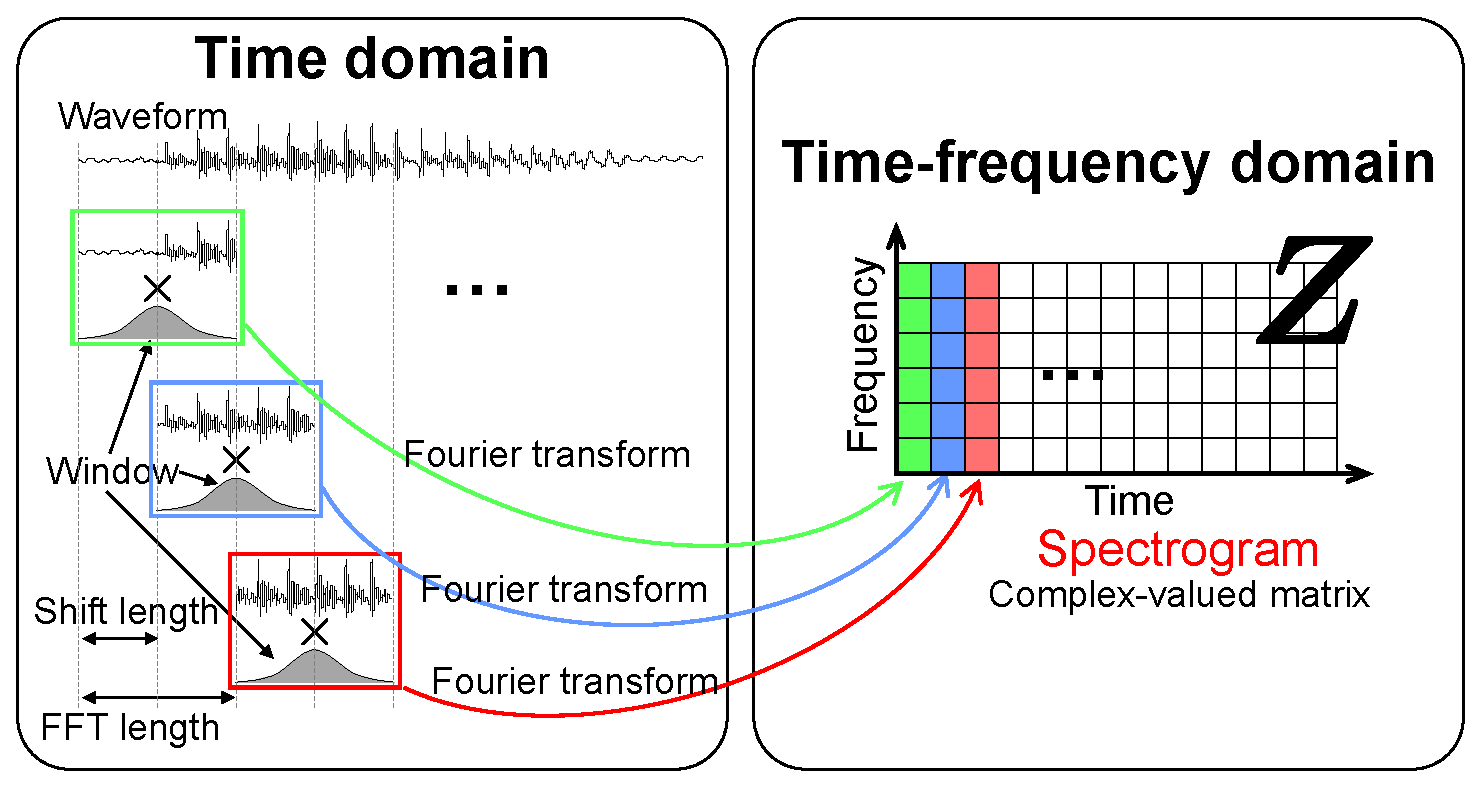
\includegraphics[width=0.95\columnwidth]{figures/stft.eps}
    \end{center}
    \vspace{-8pt}
	\caption{Mechanism of STFT.}
	\label{fig:stft}
\end{figure}
%%%%%%%%%%%%%%%%%%%%%%%%%%%%
STFTはFig.~\ref{fig:stft}に示すような時
間的に変化するスペクトルを表現するための手法である.
STFT の分析窓関数の長さ及びシフト長をそれぞれ$Q$及び$\tau$としたとき,時間領域の信号
$z(l)$の$j$番目の短時間区間(時間フレーム)の信号は次式で表される.
\begin{align}
    \bm{z}^{(j)} &= \left(z\left((j-1)\tau+1\right), z\left((j-1)\tau+2\right), \cdots , z\left((j-1)\tau+Q\right) \right)^{T}\\
    &= \left(
    z^{(j)}(1),z^{(j)}(2),\cdots , z^{(j)}(q), \cdots , z^{(j)}(Q)
    \right)^{T}~\in \mathbb{R}^{Q}
\end{align}
ここで,$j= 1, 2, \cdots , J$及び$q= 1, 2, \cdots , Q$は,それぞれ時間フレーム及び時間フレーム内のサン
プルを示す.また,セグメント数$J$は次式によって与えられる.
\begin{align}
    J = \frac{L}{\tau}
\end{align}
また,各時間フレームの信号のSTFTは次式のようにして求められる.
\begin{align}
\bm{Z}= {\rm STFT}_{\bm{\omega}}(\bm{z})~\in \mathbb{C}^{I \times J}
\end{align}
また,スペクトログラム$\bm{Z}$の$(i, j)$ 番目の要素は次式で表される.
\begin{align}
    z_{ij}= \sum_{q=1}^{Q}\omega(q)z^{(j)}(q){\rm exp}\left\{\frac{-\iota2\pi(q-1)(i-1)}{F}\right\}
\end{align}
ここで$F$は$\lfloor \frac{F}{2}\rfloor+1 =I$を満たす整数($\lfloor \cdot \rfloor$は床関数)を,$i= 1, 2, \cdots , I$は周波数ビンのインデクスを,
$\iota$は虚数単位を,$\bm{\omega}$は分析窓関数を示している.
このように,時間領域の信号は一定幅の短時間ごとに分析窓関数を乗じて離散フーリエ変換を行うことで,横軸が時間,縦軸が周波数のスペクトログラムと呼ばれる複素行列$\bm{Z}$で表すことができる.

%----------------------------------------------
\section{周波数領域におけるBSSの定式化}
\label{sec:formularization}
%----------------------------------------------
今一度,音源数と観測チャネル数(マイクロホン数)をそれぞれ$N$及び$M$とする.
また,各観測音源信号をSTFTすることで得られる,各時間周波数における音声信号,混合信号,及び分離信号をそれぞれ
\begin{align}
  \bm{s}_{ij} &= \left(
	s_{ij,1},s_{ij,2}, \cdots, s_{ij,n}, \cdots, s_{ij,N} 
  \right)^\mathrm{T}~\in \mathbb{C}^{N}\\
  \bm{x}_{ij} &= \left(
      x_{ij,1},x_{ij,2},  \cdots, x_{ij,m}, \cdots  , x_{ij,M} 
  \right)^\mathrm{T}~\in \mathbb{C}^{M} \\
  \bm{z}_{ij} &= \left(
      z_{ij,1},z_{ij,2},  \cdots, z_{ij,n}, \cdots  , z_{ij,N} 
  \right)^\mathrm{T}~\in \mathbb{C}^{N}
\end{align}
と表す.
ここで,$i= 1, 2, \cdots , I$,$j = 1, 2, \cdots , J$,$n = 1, 2, \cdots , N$,及び$m =
1, 2, \cdots , M $はそれぞれ周波数,時間,音源,チャネルのインデクスを示す.
また,複素スペクトログラム行列$\bm{S}_{n} \in \mathbb{C}^{I\times J}$, $\bm{X}_{m} \in \mathbb{C}^{I\times J}$及び$\bm{Z}_{n} \in \mathbb{C}^{I\times J}$の成分をそれぞれ
$s_{i, j, n}$, $x_{i, j, m}$及び$z_{i, j, n}$ と表す.

%----------------------------------------------
\section{FDICA}
\label{sec:fdica}
%----------------------------------------------
\ref{sec:ica}節で説明したように,ICAとは,観測信号が独立信号の線形結合として観測される場合に,各信号間の独立性を最も高めるように線形分離行列を推定することでBSSを実現する手法である.
しかし,実際に観測される音声信号には残響の影響を受けており,線形時不変なインパルス応答が畳み込まれて混合される.
インパルス応答の畳み込みは残響長$R$を用いて次式のように表される.
\begin{align}
  \bm{x}(l) = \sum_n \sum_{l^{'}=0}^{R-1} \tilde{\bm{a}}_n(l^{'}) \bm{s}_n(l-l^{'})
  \label{f:tatami}
\end{align}
ここで,$\tilde{\bm{a}}_n(l)$は,音源$n$に対する畳み込み混合係数ベクトル(音源$n$からマイクロフォン$m$までのインパルス応答をまとめたもの)である.
これを分離するためには逆畳み込みフィルタを推定することが必要となる.
一般的に逆畳み込みフィルタの推定は容易ではないことから,時間領域でのICAによるBSSは困難である.
この問題を解決するために,式(\ref{f:tatami})の時間領域における畳み込み混合を,STFTによって周波数領域上での瞬時混合に変換し,時間周波数領域で周波数毎にICAを行うFDICAが提案された.

FDICAでは,周波数毎の時不変な混合行列 $\bm{A}_{i} = (\bm{a}_{i, 1} ~\bm{a}_{i, 2} ~\cdots ~\bm{a}_{i, n}~\cdots,\bm{a}_{i, N} )\in \mathbb{C}^{M\times N}$を定義し,混合信号が次式で表現できると仮定する.
\begin{align}
 \bm{x}_{ij} = \bm{A}_i\bm{s}_{ij}
\end{align}
この混合モデルは,STFTの窓長が室内残響よりも長い場合にのみ成立する.
以後,決定的な系($M=N$)を仮定すると,混合行列$\bm{A}_{i}$が正則であれば,分離行列$\bm{W}_i=\bm{A}_i^{-1}=(\bm{w}_{i,1}~\bm{w}_{i,2}~ ...~ \bm{w}_{i, n}~ ... ~\bm{w}_{i, N})^{\mathrm{H}}$を用いて,分離信号を次式で表せる.
\begin{align}
 \bm{z}_{ij} = \bm{W}_{i}\bm{x}_{ij} \label{eq:sep}
\end{align}
ここで,$\cdot^\mathrm{H}$はベクトルや行列のエルミート転置を示す.
分離行列の行ベクトルである$\bm{w}_{i,n}\in\mathbb{C}^M$は,周波数$i$において,観測信号から$n$番目のみの音源へ変換する分離フィルタである.
このようにFDICAでは,観測信号$\bm{x}_{ij}$の各周波数ビンに対しそれぞれ独立にICA を適用することで,周波数毎の分離行列$\bm{W}_{i}$を全周波数にわたって推定することで音源分離を行う.

%----------------------------------------------
\section{パーミュテーション問題とその解決}
\label{sec:pp}
%----------------------------------------------
FDICA中で周波数毎に適用しているICAは,音源間の統計的独立性のみに基づいて分離行列を推定するため,分離音源の周波数毎のスケール及び順番に関しては不定である.
従って,FDICAの推定分離行列を$\hat{\bm{W}}_i$とすると,次式のような不定性が残る.
\begin{align}
	\hat{\bm{W}}_{i} &= \bm{D}_{i}\bm{P}_{i}  \bm{W}_{i}
\end{align}
ここで,$\bm{P}_i \in \{0, 1\}^{N \times N}$は分離行列$\bm{W}_{i}$の行ベクトル$\bm{w}_{i, n}$の順番を入れ変えうるパーミュテーション行列(置換行列)である.
$\bm{D}_i \in \mathbb{R}^{N \times N}$は,$\bm{w}_{i,n}$のスケールを変化させる可能性のある対角行列である.
すなわち,FDICAで推定される分離信号
\begin{align}
\bm{y}_{ij} &= \hat{\bm{W}}_i\bm{x}_{ij} \\
&=\left( y_{ij,1},y_{ij,2}, \cdots, y_{ij,n}, \cdots, y_{ij,N} \right)^\mathrm{T}~\in \mathbb{C}^{N} \label{eq:sepSig}
\end{align}
は,推定音源の順番やスケールが周波数毎にばらばらになっている状態である.
このうち,$\bm{D}_i$によって生じるスケールの任意性は,プロジェクションバック法\cite{Matsuoka2001_PB}で復元可能である.
一方で,$\bm{P}_i$によって生じる分離信号の順番の任意性(パーミュテーション)を純粋に復元することは,組み合わせ爆発が発生するため容易ではない.
この問題は,一般的にパーミュテーション問題と呼ばれる.
パーミュテーション問題の概要をFig.~\ref{fig:permu}に示す.
ここで,FDICAで推定される分離信号$\bm{y}_{ij}$の音源毎の複素スペクト
ログラム行列を$\bm{Y}_n \in \mathbb{C}^{I \times J}$で表している.
FDICA直後の$\bm{Y}_n$に注目すると,周波数毎での音源分離は達成できている.
しかし,時間周波数構造全体としては,異なるグループの分離信号が1つの時間周波数構造に混在していることが分かる.
これがパーミュテーション問題であり,ICAの分離信号の順番に関する不定性に起因して発生している.
そのため,FDICAにはポスト処理として,分離された音源の順番を全周波数ビンにわたって正しく並べ直す必要がある.
%%%%%%%%%%%%%%%%%%%%%%%%%%%%
\begin{figure}[t]
    \begin{center}
        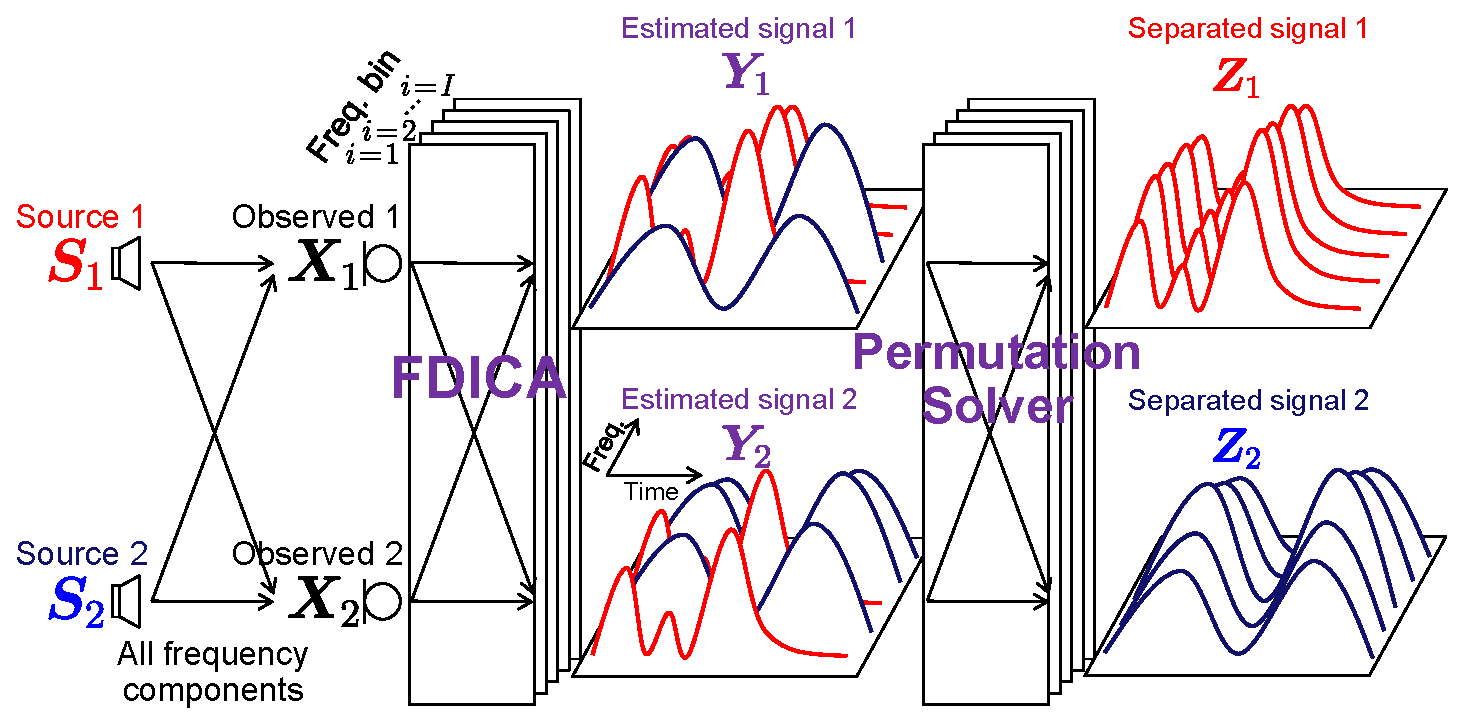
\includegraphics[width=0.95\columnwidth]{figures/permutation_image.eps}
    \end{center}
    \vspace{-8pt}
	\caption{Permutation problem in FDICA, where $N=M=2$.}
	\label{fig:permu}
\end{figure}
%%%%%%%%%%%%%%%%%%%%%%%%%%%%

パーミュテーション問題を解決して得られる分離信号は次式となる.
\begin{align}
\bm{z}_{ij} &= \bm{P}_{i}^{-1}\bm{D}_{i}^{-1}\bm{y}_{ij} \label{eq:z}
\end{align}
%本論文では,この$\bm{P}_{i}^{-1}$を推定することが目的となる.

このパーミュテーション問題を解決するために,これまでにも数々のパーミュテーション解決法が提案されてきた.
代表的な既存手法の1つに,隣接周波数の時系列強度(音源アクティベーション)の相関を用いたパーミュテーション解決法\cite{COR}がある.
これは,分離信号のパーミュテーションが正しければ,隣接した周波数アクティベーション間の相関が高くなりやすいという仮定の下で並べ替える手法である.また,離れた周波数においても,同じ音源のアクティベーション間の相関が高くなるように並び替えられている.
%り,次式のように相関を計算する.
%\begin{align}
%\Tilde{\bm{v}}_{i}(n) &=  \frac{1}{J}\sum_{j=0}^{J} |\bm{y}_{i,j,n}| \\
% {\rm sim}(i) &= \sum_{n\neq m} \frac{\Tilde{\bm{v}}_{i}(n) \cdot \Tilde{\bm{v}}_{i}(m)}{\|
% \Tilde{\bm{v}}_{i}(n)\|~\| \Tilde{\bm{v}}_{i}(m)\|}
%\end{align}
%ここで,$\cdot$は内積を表しており,
他にも,マイクロホンの相対的な位置情報を既知として音源到来方位を計算し,パーミュテーション解決の手掛かりとする手法 \cite{DOA}および両者を組み合わせたパーミュテーション解決法も提案されている.
しかしながら,パーミュテーション問題の解は組み合わせ爆発を起こすことから,上記いずれの手法を用
いても完璧にパーミュテーション問題を解くことは非常に難しく,とくに複数音声の混合信号における高精
度なパーミュテーション問題の解決はいまだできていない.

%----------------------------------------------
\section{深層パーミュテーション解決法}
\label{sec:ivailrma}
%----------------------------------------------

近年では,DNNを用いたパーミュテーション問題解決法が登場している.観測された混合信号$\bm{X}_n$にFDICA適用すると,パーミュテーション問題が生じた分離信号$\bm{Y}_n$が得られる.
これらのパワースペクトログラム$|\bm{Y}_n|^{.2}$から全周波数帯域中の局所的な狭帯域(サブバンド)を定義し,サブバンド毎にデータをDNNに入力し,パーミュテーションを解決する.
サブバンド毎に参照周波数を定義し,その近傍周波数が参照周波数に対して同一音源か否かを判断し,同一音源である場合はDNNの出力として「0」を出力し,同一音源でない場合はDNNの出力として「1」を出力する.2つの周波数これらの推定処理をFig.~に示す.
参照周波数と近傍周波数を($i,i+\omega$),短時間時系列パワー(長さ$\tau $)を以下のように集める.
\begin{align}
  %\bm{d}_{i, \omega, \gamma} &= ({\bm{r}_{i, \gamma, 1}}^\mathrm{T}, {\bm{r}_{i, \gamma, 2}}^\mathrm{T}, {\bm{g}_{i, \omega, \gamma, 1}}^\mathrm{T}, {\bm{g}_{i, \omega, \gamma,2}}^\mathrm{T} )^\mathrm{T}~\in \mathbb{R}_{\geq 0}^{4\tau \times 1},\label{eq:DNNinputVec}\\
  \bm{d}_{i, \omega, \gamma} &= ({\tilde{\bm{r}}_{i, \gamma}}^\mathrm{T}, {\tilde{\bm{g}}_{i, \omega, \gamma}}^\mathrm{T} )^\mathrm{T}~\in \mathbb{R}_{\geq 0}^{4\tau \times 1} \label{eq:DNNinputVec}\\
  \tilde{\bm{r}}_{i,\gamma} &= ({\bm{r}_{i, \gamma, 1}}^\mathrm{T}, {\bm{r}_{i, \gamma, 2}}^\mathrm{T} )^\mathrm{T}~\in \mathbb{R}_{\geq 0}^{2\tau \times 1} \label{eq:DNNinputVecRtilde}\\
  \bm{r}_{i, \gamma, n} &= ( |y_{i, (\gamma-1) \eta+1, n}|^2, |y_{i, (\gamma-1) \eta+2, n} |^2, 
  \cdots, |y_{i, (\gamma-1) \eta+\tau, n}|^2 )^\mathrm{T}~\in \mathbb{R}_{\geq 0}^{\tau \times 1}  \label{tau1}\\
  \tilde{\bm{g}}_{i,\omega,\gamma} &= ({\bm{g}_{i, \omega, \gamma, 1}}^\mathrm{T}, {\bm{g}_{i, \omega, \gamma, 2}}^\mathrm{T} )^\mathrm{T}~\in \mathbb{R}_{\geq 0}^{2\tau \times 1} \label{eq:DNNinputVecGtilde}\\
  \bm{g}_{i,\omega, \gamma, n} &= ( |y_{i+\omega, (\gamma-1) \eta+1, n}|^2, |y_{i+\omega, (\gamma-1) \eta+2, n}|^2,\cdots, |y_{i+\omega, (\gamma-1) \eta+\tau, n}|^2 )^\mathrm{T}~\in \mathbb{R}_{\geq 0}^{\tau \times 1} \label{tau2}
\end{align}
  ここで,行列の $|\cdot|^{.2}$ は,要素ごとの絶対値の二乗を返す.
  また,$\omega=-\Omega, -\Omega+1, \cdots, -1, 0, 1, \cdots, \Omega$は,$\bm{r}_{i,\gamma,n}$と$\bm{g}_{i,\omega,\gamma,n}$の周波数の差であり,$\eta$は,短時間セグメントの時間軸に沿ったストライド幅,$\gamma=1, 2, \cdots, \Gamma$は,短時間セグメントのインデクスである.
  なお,$\Gamma$は,短時間のアクティベーションの長さ$\tau$ とストライド幅$\eta$によって決まる.
  ベクトル $\bm{r}_{i,\gamma,n}$ は,参照周波数$i$の短時間時系列パワーに対応し,ベクトル $\bm{g}_{i,\omega,\gamma,n}$は,Fig.~\ref{fig:input}に示すように,隣接又は局所周波数$i+\omega$ の短時間時系列パワーに対応する.
  DNNの入力ベクトルは,(\ref{eq:DNNinputVec})を正規化したものとして次のようにして表す.
\begin{align}
  \tilde{\bm{d}}_{i, \omega, \gamma} &=\frac{\bm{d}_{i, \omega, \gamma} }{ \|{\bm{d}_{i, \omega, \gamma} }\|_2}~\in \mathbb{R}_{\geq 0}^{4\tau \times 1}  \label{eq:input}
\end{align}
提案するDNNモデルは,0または1を出力する2値分類器である.
推定結果が「0」の場合は,$\bm{r}_{i,\gamma, 1}$と$\bm{g}_{i,\omega,\gamma, 1}$が同一音源であることを意味し,同様に$\bm{r}_{i,\gamma, 2}$と$\bm{g}_{i,\omega,\gamma, 2}$も同一音源である.
一方,推定結果が「1」の場合は$\bm{r}_{i,\gamma, 1}$と$\bm{g}_{i,\omega,\gamma, 1}$(同様に$\bm{r}_{i,\gamma, 2}$と$\bm{g}_{i,\omega,\gamma, 2}$)が異なる音源成分であることを意味している.
これらの推定処理をFig.~\ref{fig:local_dnn}に示す.DNNの予測結果は次のように表せれる.
\begin{align}
  q_{i,\omega,\gamma} = \mathrm{DNN}\left(\tilde{\bm{d}}_{i,\omega,\gamma}\right) \in \{0, 1\}
\end{align}
この結果を時間方向にずらして,全時間フレームに対するDNNの予測処理を走査する.そして,DNNの予測結果を時間軸に対して多数決処理を行うことで,より信頼性の高いサブバンドベクトルを取得する.
サブバンドベクトルは,基準周波数$i$をシフトすることにより全周波数で推定する.ただ,各サブバンドベクトル内の2値は(「0」及び「1」)は異なる意味を持つ可能性がある.これはサブバンド内の周波数成分が.
参照周波数の成分と同一音源か否かを示しているに過ぎず,参照周波数の変化を共に,対応音源が変化する.2音源でサブバンドベクトル内の値が「1」,つまり同一音源ではない場合は,必然的にもう一方の音源となる.ただ,3音源以上になるとサブバンドベクトル内の値が「1」の時,残りのどの音源を一致するのかが判断できない.
そのため,3音源以上になると組み合せ爆発を起こしてしまい,計算量の観点から3音源以上の音源分離は難しい.

%----------------------------------------------
\section{本章のまとめ}
%----------------------------------------------
本章では,提案手法において必要となる基礎理論および各種従来手法について説明した.
次章以降では,より簡潔に精度の良いのBSSを達成するために\ref{sec:fdica}節で導入したFDICAのポスト処理として,DNNに基づくパーミュテーション解決法を新たに提案する.


















%%%%% 第3章 %%%%%

\chapter{提案手法}
\label{chap:proposed}

%----------------------------------------------
\section{まえがき}
%----------------------------------------------
前章では,\red{音響信号のBSSにおいて重要な}FDICA\blue{に伴い生じる}\red{の}パーミュテーション問題\blue{と従来の深層}\red{について詳しく述べた.また,音源モデルに基づきパーミュテーション問題を回避する手法や,近年提案された深層}パーミュテーション解決法について説明した.
\red{さらに,既存の深層パーミュテーション解決法では,音源数$N$の増加に伴ってアルゴリズムが極端に複雑になってしまう課題について述べた.}
本章では,\blue{組み合せ爆発を起こすことのない,DNNを用いたデータ駆動型パーミュテーション解決法を新たに提案する.}
\red{音源数$N$が増加した場合でもアルゴリズムが複雑化することのない深層パーミュテーション解決法を新たに提案する.}
\red{まず\ref{sec:moti}節では,BSSにおいて深層学習を用いてパーミュテーション問題の解決を目指す動機について述べる.}
\ref{sec:in-out}節及び\ref{sec:model}節で\red{は},\red{本論文で提案する深層}パーミュテーション解決法\red{の}DNNモデルの入出力及び\red{ネットワーク}構造を\red{それぞれ}説明する.
\ref{sec:loss}節及び\ref{sec:maj}節では,誤差逆伝播に用いる損失\red{関数}の取り方と\blue{パーミュテーション行列の並び替えに用いる}\red{パーミュテーション行列を正確に推定するモデルを学習するための}\blue{ラベルの取得方法}\red{入力データ及び正解データ(ラベル)の取得方法}を\red{それぞれ}説明する.
\ref{sec:3matome}節で本章のまとめを述べる.

%----------------------------------------------
\section{動機}
\label{sec:moti}
%----------------------------------------------
%%%%%%%%%%%%%%%%%%%%%%%%%%%%
\begin{figure}[t]
    \begin{center}
        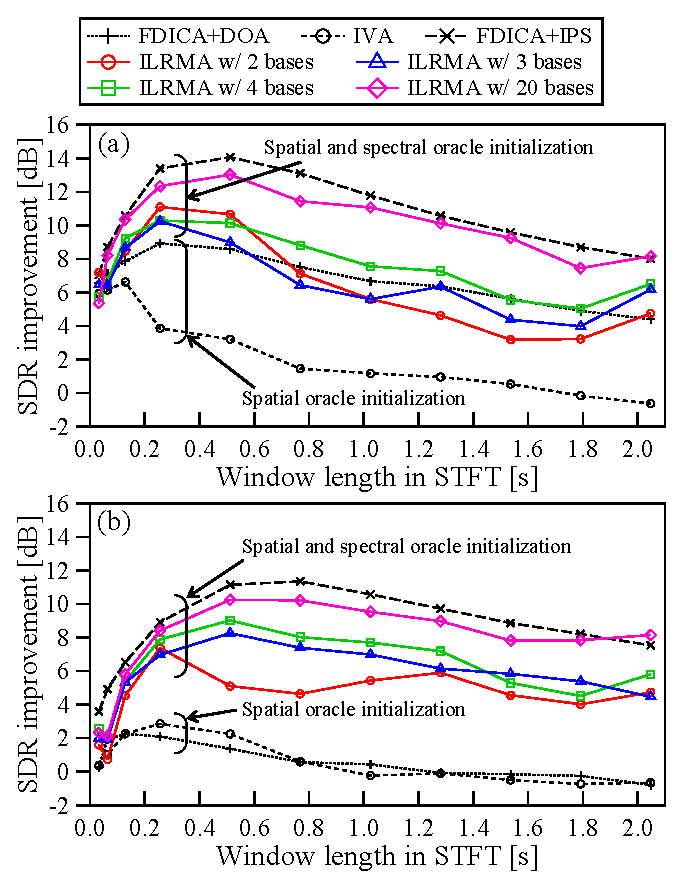
\includegraphics[width=0.8\columnwidth]{figures/SpeechE2AJR2_opt12+note.eps}
    \end{center}
    \vspace{-8pt}
	\caption{Average source separation results for speech signals using random initialization: (a) E2A (\red{$T_{60} = 300$~ms}) and (b) JR2 (\red{$T_{60}=470$~ms}) impulse responses. \red{For details of this figure, see~\cite{EU}.}}
	\label{fig:kitamura_es}
\end{figure}
%%%%%%%%%%%%%%%%%%%%%%%%%%%%

文献~\cite{EU}では,\red{IVAやILRMAに基づく}BSSのSTFTにおける最適な\blue{窓長を}\red{短時間区間長(窓長)$Q$について}実験的に\blue{検討}\red{調査}している.
Fig.~\ref{fig:kitamura_es}(b)は,文献~\cite{EU}の実験結果の図を引用したものである.\red{詳しい実験条件等は文献\cite{EU}を参照されたい.}縦軸は信号対歪み比(source-to-distortion ratio: SDR)\cite{BSSEval}の改善量であり,これは即ち\blue{分離性能}\red{音源分離の性能}を表している.
この結果より,IVA及びILRMAでは,残響\blue{状態}\red{時間が}\blue{{$T_{60} = $}}$470~\mathrm{ms}$\blue{の条件}\red{という比較的残響の強い条件}では\red{,IVAもILRMAも高精度な音源}分離に失敗していることが分かる.
一方で,FDICAに対して,音源信号$\bm{s}_{ij}$を用いる理想的なパーミュテーション解決法(ideal permutation solver: IPS)を適用した結果\red{(すなわちFDICAの達成しうる限界性能)}では10~dB以上のSDRの改善を達成している.
この事実は,高残響下での\blue{音声混合信号}\red{音声信号の混合という難しい観測条件}であっても,$\hat{\bm{W}}_i$\blue{はFDICAで正確に推定でき,}\red{の推定自体(すなわち周波数ビン毎のBSS)はFDICAでも高精度に実現できていることを示している.すなわち,残る課題は推定信号$\bm{y}_{ij}$を正しい順番に並び変えるパーミュテーション問題の解決(}
$\bm{P}_i^{-1}$の\blue{推定のみ失敗していることを示している.}
\red{推定)のみであることを示唆している.}
また,\red{\ref{sec:DNNs}節で述べた通り,}従来の深層パーミュテーション解決法では,\blue{全周波数帯域中の局所的な狭帯域のおける}\red{サブバンド内の}パーミュテーション問題\blue{の解決を全時間方向と全周波数方向に行う際に,}
\red{を解決する際に,}\blue{ある}参照周波数\red{ビン}に対して\blue{同一か否かで音源を判断しているため,3音源以上の分離等の拡張性に欠ける.}
\red{その他の周波数ビンの推定信号成分が同一音源の成分か否かの2クラス分類問題をDNNで予測している.音源数が$N=2$であれば,この「同一音源の成分か否か」の2クラス分類はすなわち「どちらの音源の成分か」に一致するが,音源数が$N\geq 3$となった場合は,
「同一音源の成分ではない」とDNNが判断した場合にその成分がどの音源の成分かが確定しない.従って,この場合に各推定成分がどの音源に対応するかを確定させるためには,先の2クラス分類DNNモデルを音源数$N$個の中から2つ選ぶ組み合わせ数(${}_N C_2$)分適用せねばならず,
さらに後段のサブバンド間のパーミュテーション問題の解決(全サブバンドのスティッチング)の処理を考えると,そのアルゴリズムは非常に複雑・煩雑になってしまう.
}

そこで,本論文では,簡潔なアルゴリズムでパーミュテーション問題を正確に解くことに焦点を当て,新しい\blue{DNNに基づくデータ駆動型(教師あり)パーミュテーション解決法}\red{深層パーミュテーション解決法}を提案する.
以後,本論文では,提案するパーミュテーション問題の解決法が実現可能かどうかを\blue{判断するために,}\red{判断するための基礎的な調査として,}FDICAを適応した後の分離信号\blue{に}\red{を}模倣した人工データと
実際の\blue{音声データ}\red{音響信号}を用いてパーミュテーション問題の\blue{解決を考える}\red{解決性能を実験的に調査する}.
\blue{この際,音源数{$N=2$}及びチャネル数{$M=2$}と仮定し,実験を行う.}
\red{提案手法は,音源数$N$の増加に対してアルゴリズムが極端に複雑化しない手法として提案するが,本論文は基礎的な実験に終始するため,音源数及びチャネル数が$N=M=2$の状況のみを取り扱う.$N\geq 3$以上の条件での調査については今後の課題となる.}

\blue{提案する}\red{本論文で提案する深層}パーミュテーション解決法\blue{の概要}\red{を適用する処理の概要}は以下の通りである.
\red{
\begin{enumerate}
\renewcommand{\labelenumi}{(\alph{enumi})}
    \item \red{パーミュテーション問題が未解決の状態である推定信号{$\bm{Y}_1$及び$\bm{Y}_2$}に対し,両信号のパワー比に基づく正規化\cite{Permutation_solverBSS}を施す}
    \item \red{正規化された両信号のスペクトログラムから,ある時間フレーム$j$とその前後$j\pm\beta$の時間フレームの部分的なスペクトログラムを抽出し,時間フレーム$j$を中心とした局所時間振幅スペクトログラムを両信号で構成する}
    \item \red{両信号の局所時間振幅スペクトログラムをベクトル化し,DNNに入力する.}
    \item \red{DNNは入力ベクトル中の$\bm{Y}_1$及び$\bm{Y}_2$の正規化局所時間振幅スペクトログラムの各周波数ビンの成分がそれぞれどの音源信号に属するかを分類問題として予測し,周波数毎及び音源毎の確率値をまとめたベクトルを出力する}
    \item \red{(b)--(d)の処理を全時間フレームに対して適用し,時間フレーム毎の確率値ベクトルを取得する}
    \item \red{全時間フレームの確率値ベクトルを用いて時間方向に多数決処理を適用し,全時間フレーム共通の(1本の)確率値ベクトルを得る}
    \item \red{確率値ベクトルから周波数毎のパーミュテーション行列$\bm{P}_i$の推定値$\hat{\bm{P}}_i$を構成する}
    \item \red{式(\ref{eq:z})よりパーミュテーション問題が解決された分離信号を得る}
\end{enumerate}
}
\blue{提案するパーミュテーション解決法では,全周波数成分を持ったミニ振幅スペクトログラムに対して,どの音源の成分が入っているかをDNNで予測し,その予測結果に基づいてパーミュテーション解決を行う.また,}
\red{上記の処理の詳細やDNNの学習方法については,次節以降で詳しく述べる.}
\blue{DNNには大量の学習用データが必要であるが,IPSで理想的にパーミュテーション解決された分離信号{$\bm{Z}_n$}を周波数毎にランダムにシャッフルすることで,容易かつ大量に生成することができる.}
%----------------------------------------------
\section{DNNの入出力}
\label{sec:in-out}
%----------------------------------------------
%%%%%%%%%%%%%%%%%%%%%%%%%%%%
\begin{figure}[t]
    \begin{center}
        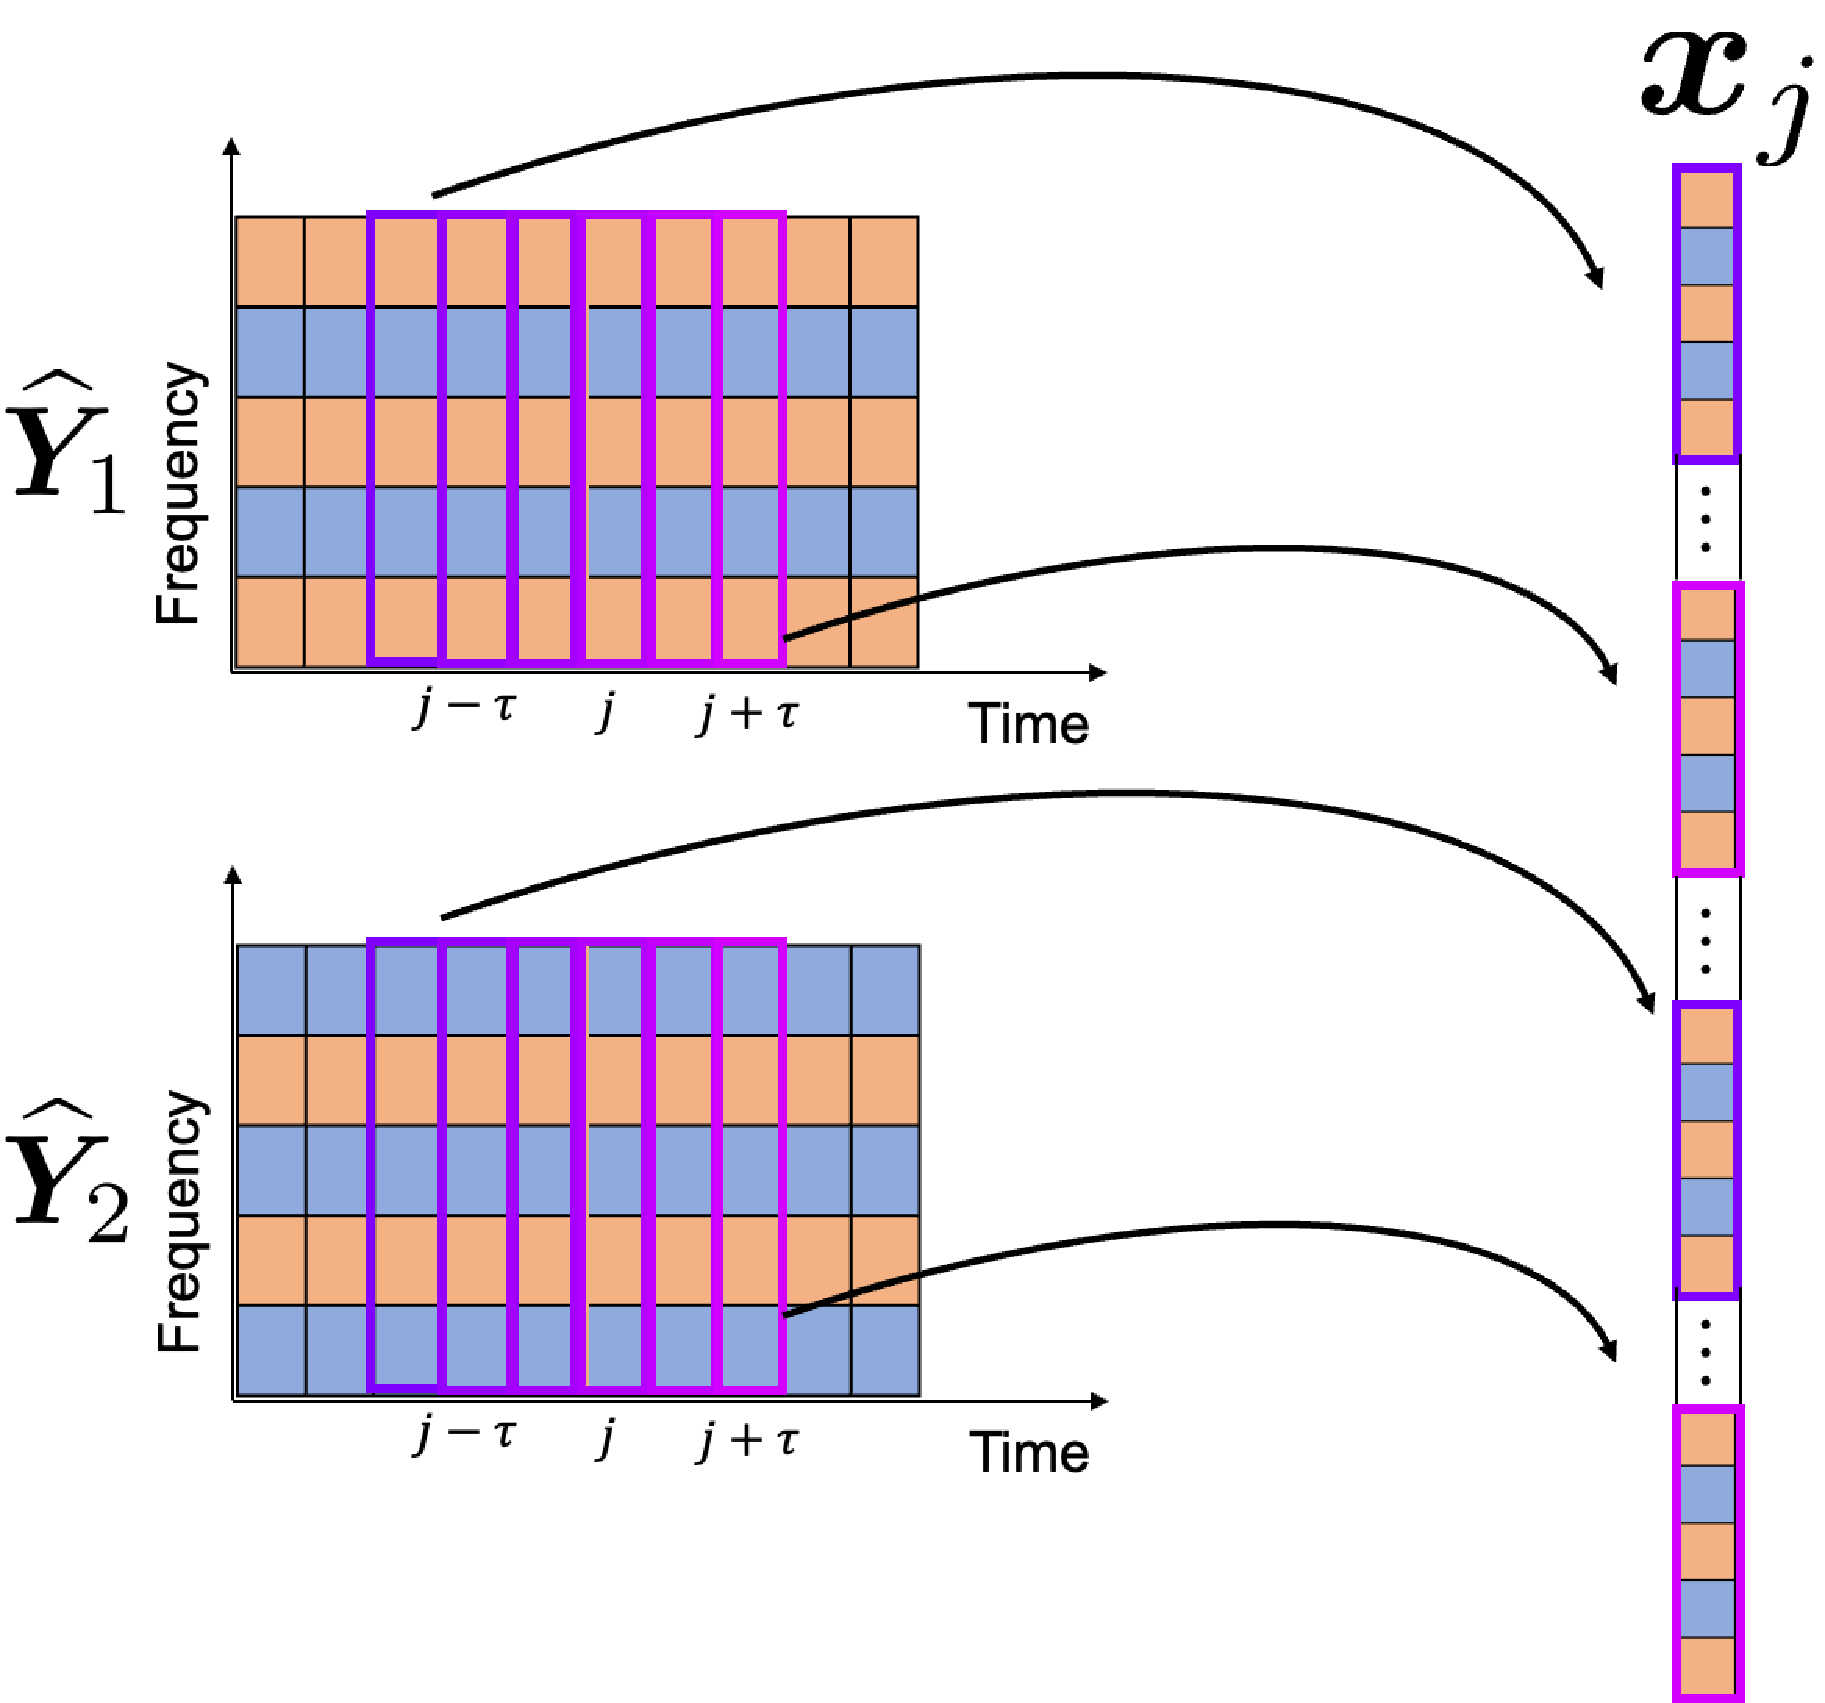
\includegraphics[height=0.8\columnwidth]{figures/DNN_input.pdf}
    \end{center}
    \vspace{-8pt}
	\caption{Input vector of DNN.}
	\label{fig:DNN_input}
\end{figure}
%%%%%%%%%%%%%%%%%%%%%%%%%%%%
提案する深層パーミュテーション解決法で用いられるDNNは複数の全結合層からなる多層パーセプトロン(multi-layer perceptron: MLP)を想定している.
MLPの入出力はあらかじめ決められた次元数のベクトルでなければならない.今,観測信号$(\bm{X}_1, \bm{X}_2)$にFDICAを適用した場合を考える.FDICAからは,パーミュテーション問題\red{が発生した状態の推定信号$(\bm{Y}_1, \bm{Y}_2)$が得られる.}
\red{ここで,同一音源に属する成分の相関を強調するため,推定信号$(\bm{Y}_1, \bm{Y}_2)$をパワースペクトログラム$(|\bm{Y}_1|^{.2}, |\bm{Y}_2|^{.2})$の比率に変換する正規化\cite{Permutation_solverBSS}を施す.この処理は次式で表される.}
\begin{align}
    \red{\overline{\bm{Y}}_1 = \frac{|\bm{Y}_1|^{.2}}{|\bm{Y}_1|^{.2}+|\bm{Y}_2|^{.2}}} \in [0,1]^{I \times J}\\
    \red{{\overline{\bm{Y}}_2 = \frac{|\bm{Y}_2|^{.2}}{|\bm{Y}_1|^{.2}+|\bm{Y}_2|^{.2}}} \in [0,1]^{I \times J}}
\end{align}
ここで,\red{行列に対する絶対値記号は要素毎の絶対値,行列やベクトルに対するドット付き指数乗は要素毎の指数乗,及び行列間のベクトルは要素毎の商を示している.}
\red{このような正規化は,文献\cite{Permutation_solverBSS}で詳しく解析されているように同一音源に属する成分の相関を強調させる利点があるだけでなく,推定信号の値が区間$[0,1]$の範囲に限定されることから,DNNの学習を安定させる効果も期待できる.}
\red{次に,推定信号の正規化振幅スペクトログラム$(\overline{\bm{Y}}_1, \overline{\bm{Y}}_2)$から,Fig.~\ref{fig:make_minispec}に示すように,時間フレーム$j$を中心とする局所時間振幅スペクトログラムを抽出する.この処理は次式で表される.}
%%%%%%%%%%%%%%%%%%%%%%%%%%%%
\begin{figure}[t]
    \begin{center}
        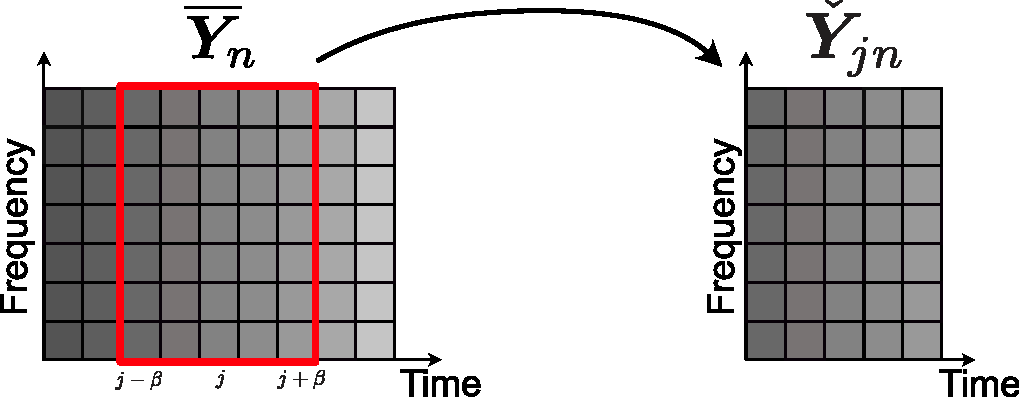
\includegraphics[width=0.95\columnwidth]{figures/make_minispec.pdf}
    \end{center}
    \vspace{-8pt}
	\caption{Extraction of local-time-frame amplitude spectrogram.}
	\label{fig:make_minispec}
\end{figure}
%%%%%%%%%%%%%%%%%%%%%%%%%%%%
\begin{align}
    \check{\bm{Y}}_{j1} &= [ \overline{\bm{y}}_{(j-\beta)1}, \overline{\bm{y}}_{(j-\beta+1)1}, \cdots, \overline{\bm{y}}_{(j-1)1}, \overline{\bm{y}}_{j1}, \overline{\bm{y}}_{(j+1)1}, \cdots, \overline{\bm{y}}_{(j+\beta)1}  ] \in [ 0, 1 ]^{I\times (2\beta+1)} \label{eq:y_check1}\\
    \check{\bm{Y}}_{j2} &= [ \overline{\bm{y}}_{(j-\beta)2}, \overline{\bm{y}}_{(j-\beta+1)2}, \cdots, \overline{\bm{y}}_{(j-1)2}, \overline{\bm{y}}_{j2}, \overline{\bm{y}}_{(j+1)2}, \cdots, \overline{\bm{y}}_{(j+\beta)2}  ] \in [ 0, 1 ]^{I\times (2\beta+1)} \label{eq:y_check2}
\end{align}
ここで,$\overline{\bm{y}}_{jn}\in [0,1]^{I}$は正規化振幅スペクトログラム$\overline{\bm{Y}}_n$の$j$列目の列ベクトル(時間フレーム$j$の正規化振幅スペクトル)を表す.
また,$\beta$(0以上の整数)は時間フレーム$j$の近傍時間フレームをどの程度DNNに入力するかを決めるパラメータである.
\red{提案手法では,DNNの入力ベクトル}は,
\red{式(\ref{eq:y_check1})及び(\ref{eq:y_check2})で得られる両信号の正規化局所時間振幅スペクトログラム$(\check{\bm{Y}}_{j1}, \check{\bm{Y}}_{j2})$をFig.~\ref{fig:DNN_input}のように一次元に整形(ベクトル化)したベクトルである.}
\blue{これを{$\bm{x}_j$}とおくと,次式のように構成される.}
\red{入力された行列をベクトル化する処理を$\mathrm{vec}(\cdot)$と表記すると,DNNの入力ベクトルは次式となる.}
\begin{align}
    \red{\bm{d}_j = \begin{bmatrix}
        \mathrm{vec}( \check{\bm{Y}}_{j1} ) \\
        \mathrm{vec}( \check{\bm{Y}}_{j2} )
      \end{bmatrix}
    \in [0,1]^{2I(2\beta+1)}}
\end{align}

\red{DNNによる予測は次式で表される.}
\begin{align}
    \red{\hat{\bm{l}}_j = \mathrm{DNN}(\bm{d}_j) \in [ 0, 1 ]^{2I}}
\end{align}
%%%%%%%%%%%%%%%%%%%%%%%%%%%%
\begin{figure*}[!t]
    \centering
    \subfloat[Calculatation of predicted permutation matrix.]{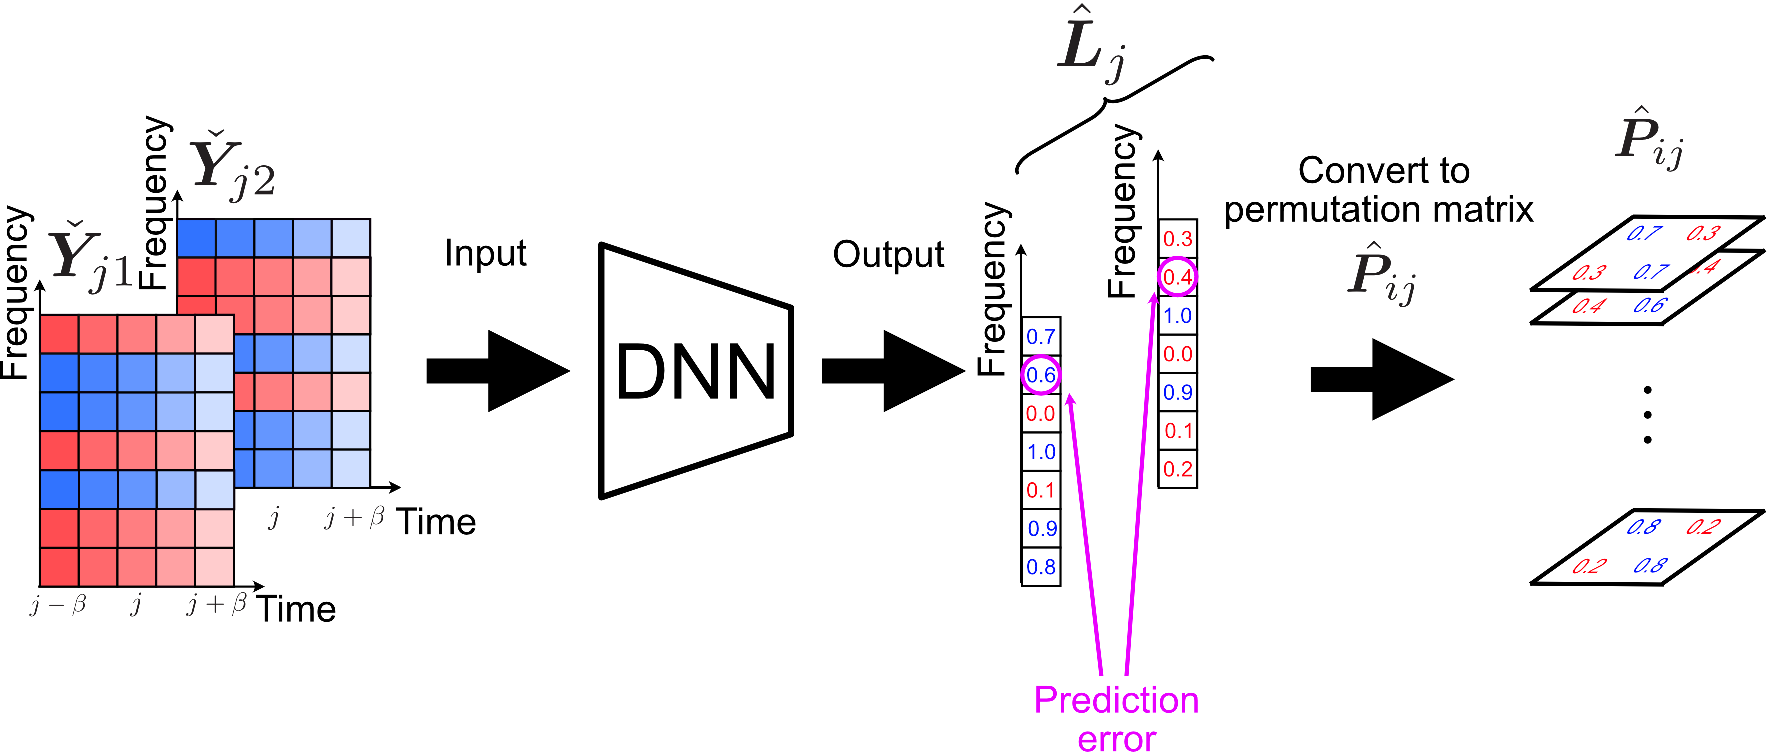
\includegraphics[clip, width=5.0in]{figures/cal_loss1.pdf}
    \label{fig:loss_process1}}
    \\
    \subfloat[Calculation of MSE with PIT.]{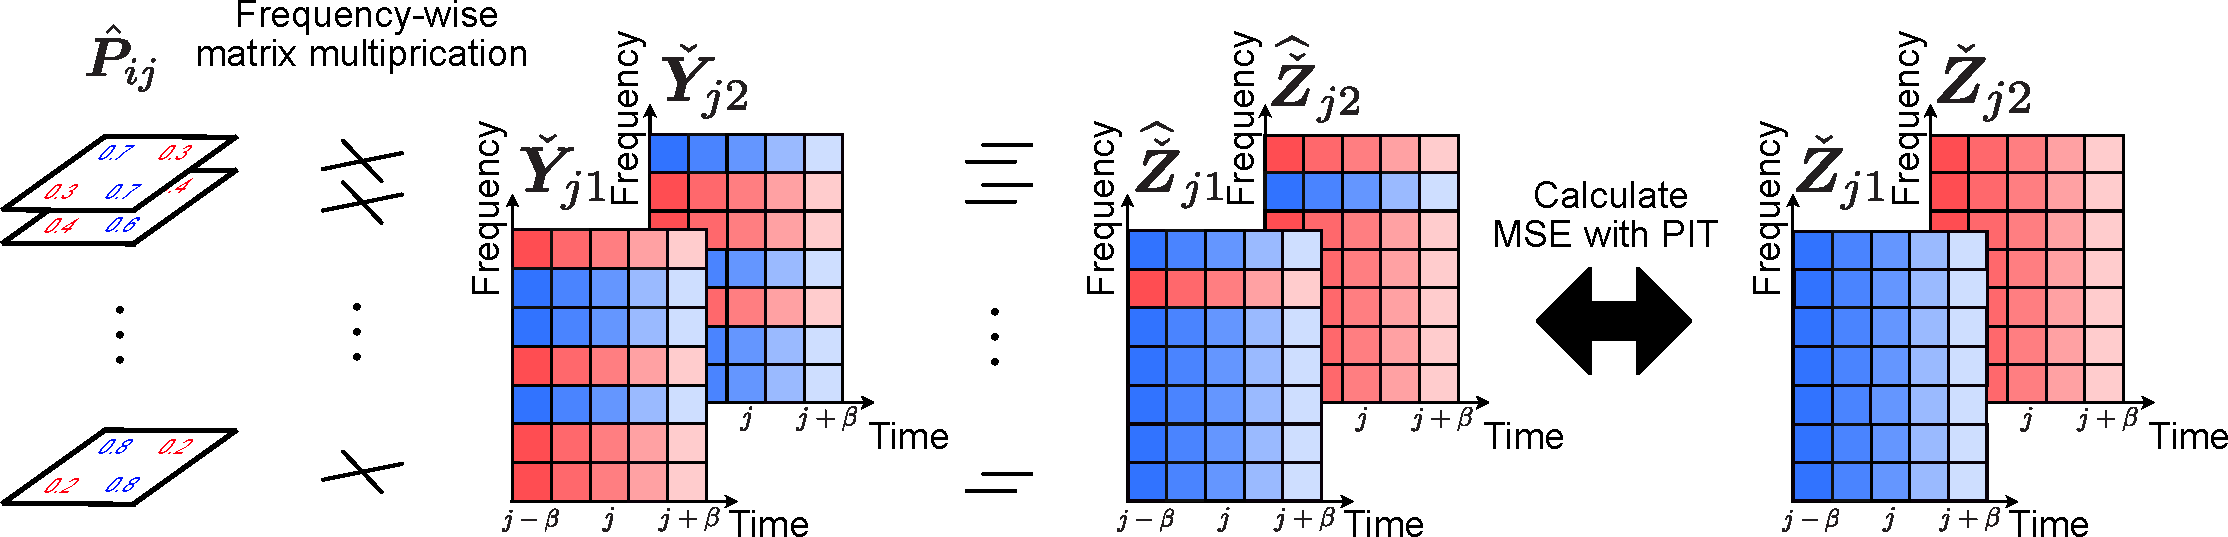
\includegraphics[clip, width=5.0in]{figures/cal_loss2.pdf}
    \label{fig:loss_process2}}  
    \caption{Process of calculating predicted permutation matrix and loss function value.}
    \label{fig:loss}
\end{figure*}
%%%%%%%%%%%%%%%%%%%%%%%%%%%%
\red{ここで,$\hat{\bm{l}}_j = [ \hat{l}_{11j}, \hat{l}_{21j}, \cdots, \hat{l}_{I1j}, \hat{l}_{12j}, \hat{l}_{22j}, \cdots, \hat{l}_{I2j} ]^\mathrm{T}$は出力である予測ベクトルを表す.
入力されたベクトルを行列化する処理を$\mathrm{mat}(\cdot)$と表記すると,予測ベクトルは次式で再成型される.
\begin{align}
  \hat{\bm{L}}_j = \mathrm{mat}(\hat{\bm{l}}_j) \in [0, 1]^{I \times 2}
\end{align}
再成型された行列$\hat{\bm{L}}_j$はFig.~\ref{fig:loss_process1}に示すように,2つのパーミュテーション問題が生じている入力信号$(\check{\bm{Y}}_{j1}, \check{\bm{Y}}_{j2})$の各周波数成分のそれぞれが
「1番目の音源の成分である確率$l_{i1}$」と「2番目の音源の成分である確率$l_{i2}$」を$\bm{d}_j$から予測したものと定義し,提案手法ではこの定義に基づいて正確な予測ができるDNNを学習する.
ここで,$(l_{i1}, l_{i2})$は離散確率値であるため$l_{i1}+l_{i2}=1$を満たし,それらの予測値である$(\hat{l}_{i1j}, \hat{l}_{i2j})$もまた$\hat{l}_{i1j}+\hat{l}_{i2j}=1$を満たすようにDNNの中で制約する必要がある.
この制約は次節で述べる通り,softmax関数を用いて実現できる.また,詳細は後述するが,パーミュテーション問題の解は時間方向には変化しない(式(\ref{eq:w_fdica})における$\bm{P}_i$は時間フレーム$j$によらない時不変行列である)ため,
様々な局所時間振幅スペクトログラムの入力$\bm{d}_j$の予測結果$\hat{\bm{L}}_j$を$j$に関して多数決処理することで,より精度の高い予測である予測結果$\hat{\bm{L}}$(この結果は$j$によらない)を生成できる.
}

\red{
重要なこととして,確率値$(l_{i1}, l_{i2})$は式(2.27)で述べたパーミュテーション行列それ自身と本質的に等価である.従って,DNNの予測結果である$(\hat{l}_{i1}, \hat{l}_{i2})$から推定パーミュテーション行列を次式で構成できる.
\begin{align}
  \hat{\bm{P}}_{i} = 
  \begin{bmatrix}
    \hat{l}_{i1} & \hat{l}_{i2} \\
    \hat{l}_{i2} & \hat{l}_{i1}
  \end{bmatrix} \label{eq:estPermMat}
\end{align}
ここで,$\hat{l}_{i1}$及び$\hat{l}_{i2}$は$\hat{\bm{L}}$の要素である.正解のパーミュテーション行列は順列を並び替える行列であるため,$N=2$の場合は式(\ref{eq:permu_mat_2dim})のいずれかとなる.
推定パーミュテーション行列$\hat{\bm{P}}_{i}$は式\eqref{eq:estPermMat}であるため,予測が不完全であれば$\bm{I}$又は$\bm{1}-\bm{I}$にはならない可能性があるが,
それでも$\hat{l}_{i1}+\hat{l}_{i2}=1$を満たすため,二重確率行列(doubly stochastic matrix: DSM)であることがわかる.
また,Birkhoff--von Neumannの定理(付録\ref{chap:vonNeumann}参照)を考慮すると,パーミュテーション問題の発生している入力データからDSMを予測する提案手法のDNNは,
考えうる全てのパーミュテーション行列に対する凸結合係数を推定していることになる.
即ち,考えうるパーミュテーション行列の中でどの行列が正解かという確信度を予測していると解釈することもできる.
}

%----------------------------------------------
\clearpage
\section{DNNの構造}
\label{sec:model}
%----------------------------------------------
%%%%%%%%%%%%%%%%%%%%%%%%%%%%
\begin{figure}[t]
    \begin{center}
        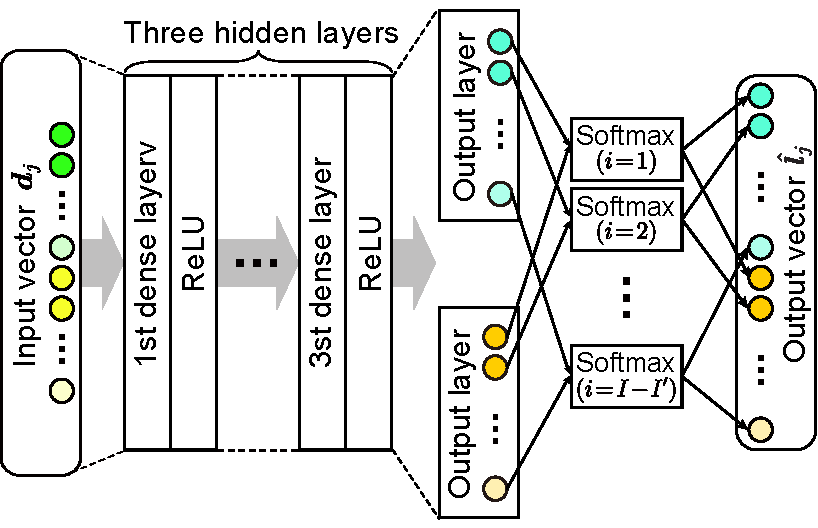
\includegraphics[width=0.8\columnwidth]{figures/architecture_DNN.pdf}
    \end{center}
    \vspace{-8pt}
	\caption{DNN architecture.}
	\label{fig:Dnnmodel}
\end{figure}
%%%%%%%%%%%%%%%%%%%%%%%%%%%%

Fig.~\ref{fig:Dnnmodel}に提案深層パーミュテーション解決法で用いるDNNの構造を示す.
このDNNは,入力層,隠れ層3層,及び出力層の計5層\red{の全結合層(dense layer)}からなる\blue{全結合構成}\red{MLP}となっており,\blue{1~5番目の隠れ層には}\red{隠れ層の1層目から3層目には非線形関数として}rectified linear unit (ReLU)~\cite{relu} 関数
\red{を用いている.
また,3層目の隠れ層から出力層に変換する際には,Fig.~\ref{fig:Dnnmodel}に示すように2つの$I$次元ベクトルに分岐させている.この時の各ベクトルへの変換パラメータは独立している\footnote{すなわち,$2I$次元への全結合層による変換と同様であるが,明示的に分岐させて定義している.}.
その後,2つの$I$次元の同一インデクスの要素に対してsoftmax関数を適用することで,予測ベクトルの全要素が閉区間$[0,1]$内の値かつ同一インデクスの要素の和が1となることを保証している.
これは,前節で説明した$\hat{l}_{i1}+\hat{l}_{i2}=1$の制約を保証することに対応し,これによって予測ベクトルを確率値としてみなすことが可能となる.}
\blue{最終隠れ層にはsoftmax関数を適用している.}
\blue{各隠れ層の次元数は全て,4096である.}

%----------------------------------------------
\section{\red{DNN学習時の損失関数}}
\label{sec:loss}
%----------------------------------------------
\red{DNNの学習は,何らかの損失関数を定義しその値を最小化するパラメータを誤差逆伝播により推定する処理となる.提案手法のDNNは\ref{sec:in-out}節で述べた通り,入力データから周波数毎の正しい音源パーミュテーションを予測するモデルである.
これは(音源数が$N=2$であれば)$(l_{i1}, l_{i2})$の2クラス分類器であるため,softmax関数を用いて各クラスへの確率値を出力している.
通常,多クラス分類器の損失関数には,カテゴリカル分布\footnote{多項分布における試行回数を1回とした際の分布である.}の負対数尤度関数であるカテゴリカル交差エントロピー(categorical cross entropy: CCE)を用いることで,DNNの学習を最尤推定の枠組みで行うことができる.
しかしながら,提案手法の深層パーミュテーション解決法の本来の目的は,全周波数ビンにおいてパーミュテーション行列を正確に予測することではなく,分離信号$(\bm{Z}_1, \bm{Z}_2)$を正確に予測することである.
例えば,推定信号$(\bm{Y}_1, \bm{Y}_2)$のどちらにもエネルギーがほとんど無いような周波数ビンは,実際は誤った分離信号の順序となっていても得られる分離信号$(\bm{Z}_1, \bm{Z}_2)$の音源分離精度には影響しない.
もしCCEでDNNの損失関数を定義すると,このようなエネルギーが少ない(音源分離にとって重要ではない)周波数ビンのパーミュテーション予測精度と,
大きなエネルギーを有する(音源分離にとって重要な)周波数ビンの予測精度が等しい重要度で扱われることになるため,音源分離性能向上の妨げとなる可能性がある.}

\red{そこで提案手法では,下記で説明する通り,DNNで予測された音源パーミュテーションに基づいて推定信号$(\bm{Y}_1, \bm{Y}_2)$を並び替えた予測分離信号$(\hat{\bm{Z}}_1, \hat{\bm{Z}}_2)$と正解の分離信号$(\bm{Z}_1, \bm{Z}_2)$の間の平均二乗誤差(mean squared error: MSE)を示す.}

\red{Fig.~\ref{fig:loss_process1}に損失関数の計算の処理の流れを示す.まず,予測結果に対応する行列$\hat{\bm{V}} \in \mathbb{R}^{R\times C}$とラベルに対応する行列$\bm{V} \in \mathbb{R}^{R\times C}$の間のMSEを次式で定義する.}
\red{
\begin{align}
    \mathrm{MSE}(\hat{\bm{V}}, \bm{V}) &= \frac{ 1 }{ RC } \| \hat{\bm{V}} - \bm{V} \|_\mathrm{Fr}^2 \\
    &= \frac{ 1 }{ RC } \sum_{r, c} \left( \hat{v}_{rc} - v_{rc} \right)^2 \label{eq:mseLoss}
\end{align}
ここで,$\hat{v}_{rc}$及び$v_{rc}$はそれぞれ行列$\hat{\bm{V}}$及び$\bm{V}$の要素,$r = 1, 2, \cdots, R$及び$c = 1, 2, \cdots, C$はそれぞれ行列$\hat{\bm{V}}$及び$\bm{V}$の行と列のインデクス,$\|\cdot\|_\mathrm{Fr}$はFrobeniusノルムである.
次に,Fig.~\ref{fig:loss_process1}に示すように,DNNの入力である正規化局所時間振幅スペクトログラム$(\check{\bm{Y}}_{j1}, \check{\bm{Y}}_{j2})$に対する予測結果$\bm{L}_j$と式(\ref{eq:estPermMat})を用いて,
($j$を中心とする局所時間フレームの)推定局所時間パーミュテーション行列$\hat{\bm{P}}_{ij}$を構成する.また,Fig.~\ref{fig:loss_process2}に示すように,式(\ref{eq:w_fdica})で音源パーミュテーションを並び替えた予測分離信号$(\widehat{\check{\bm{Z}}}_{j1}, \widehat{\check{\bm{Z}}}_{j2})$を求める.
さらに,この予測分離信号に対する正解ラベル(Fig.~\ref{fig:make_minispec}と同様の手順で,分離信号$(\bm{Z}_1, \bm{Z}_2)$から$j$を中心とする局所時間フレームの局所時間振幅スペクトログラムを抽出した行列)を$(\check{\bm{Z}}_{j1}, \check{\bm{Z}}_{j2})$と定義する.
これらの信号と式\eqref{eq:mseLoss}を用いて,前述の誤差関数$\mathcal{L}$は,$(\widehat{\check{\bm{Z}}}_{j1}, \widehat{\check{\bm{Z}}}_{j2})$及び$(\check{\bm{Z}}_{j1}, \check{\bm{Z}}_{j2})$間のMSEとして次式で表せる.
\begin{align}
    \mathcal{L} &= \mathrm{MSE}(\widehat{\check{\bm{Z}}}_{j1}, \check{\bm{Z}}_{j1}) + \mathrm{MSE}(\widehat{\check{\bm{Z}}}_{j2}, \check{\bm{Z}}_{j2}) \label{eq:dnnLossWithoutPit}
\end{align}
}
\red{但し,パーミュテーション問題の解決は全周波数で推定音源成分を正しく並び替えることだけが目標であり,並び替えた後の分離信号そのものの順序は予測の対象としない.
すなわち,深層パーミュテーション解決法を適用した結果が,$(\bm{Z}_1, \bm{Z}_2)$及び$(\bm{Z}_2, \bm{Z}_1)$のどちらの順序で出力されようとも構わない.
式\eqref{eq:dnnLossWithoutPit}で損失関数を定義した場合,分離信号は必ず$(\bm{Z}_1, \bm{Z}_2)$という順序で予測することをDNNに強いているため,
この問題を解消するために順序不変学習(permutation invariant training: PIT)\cite{PIT}を導入する.具体的には,損失関数を次式で定義する.
\begin{align}
  \mathcal{L} &= \min \left( \mathrm{MSE}(\widehat{\check{\bm{Z}}}_{j1}, \check{\bm{Z}}_{j1}) + \mathrm{MSE}(\widehat{\check{\bm{Z}}}_{j2}, \check{\bm{Z}}_{j2}),  \mathrm{MSE}(\widehat{\check{\bm{Z}}}_{j1}, \check{\bm{Z}}_{j2}) + \mathrm{MSE}(\widehat{\check{\bm{Z}}}_{j2}, \check{\bm{Z}}_{j1}) \right) \label{eq:dnnLossWithPit}
\end{align}
ここで,$\min (\cdot, \cdot)$は複数のスカラー引数の中で最小値を返す処理を表す.この関数の誤差逆伝播は自動微分により実装される.このように,PITを導入することで,周波数ビン間のパーミュテーション問題さえ解決されれば良く分離信号そのものの出力の順序には依存しないような学習が可能となる.
}

%----------------------------------------------
\section{\red{学習済のDNNのテストデータへの適用}}
\label{sec:maj}
%----------------------------------------------
%%%%%%%%%%%%%%%%%%%%%%%%%%%%
\begin{figure}[t]
    \begin{center}
        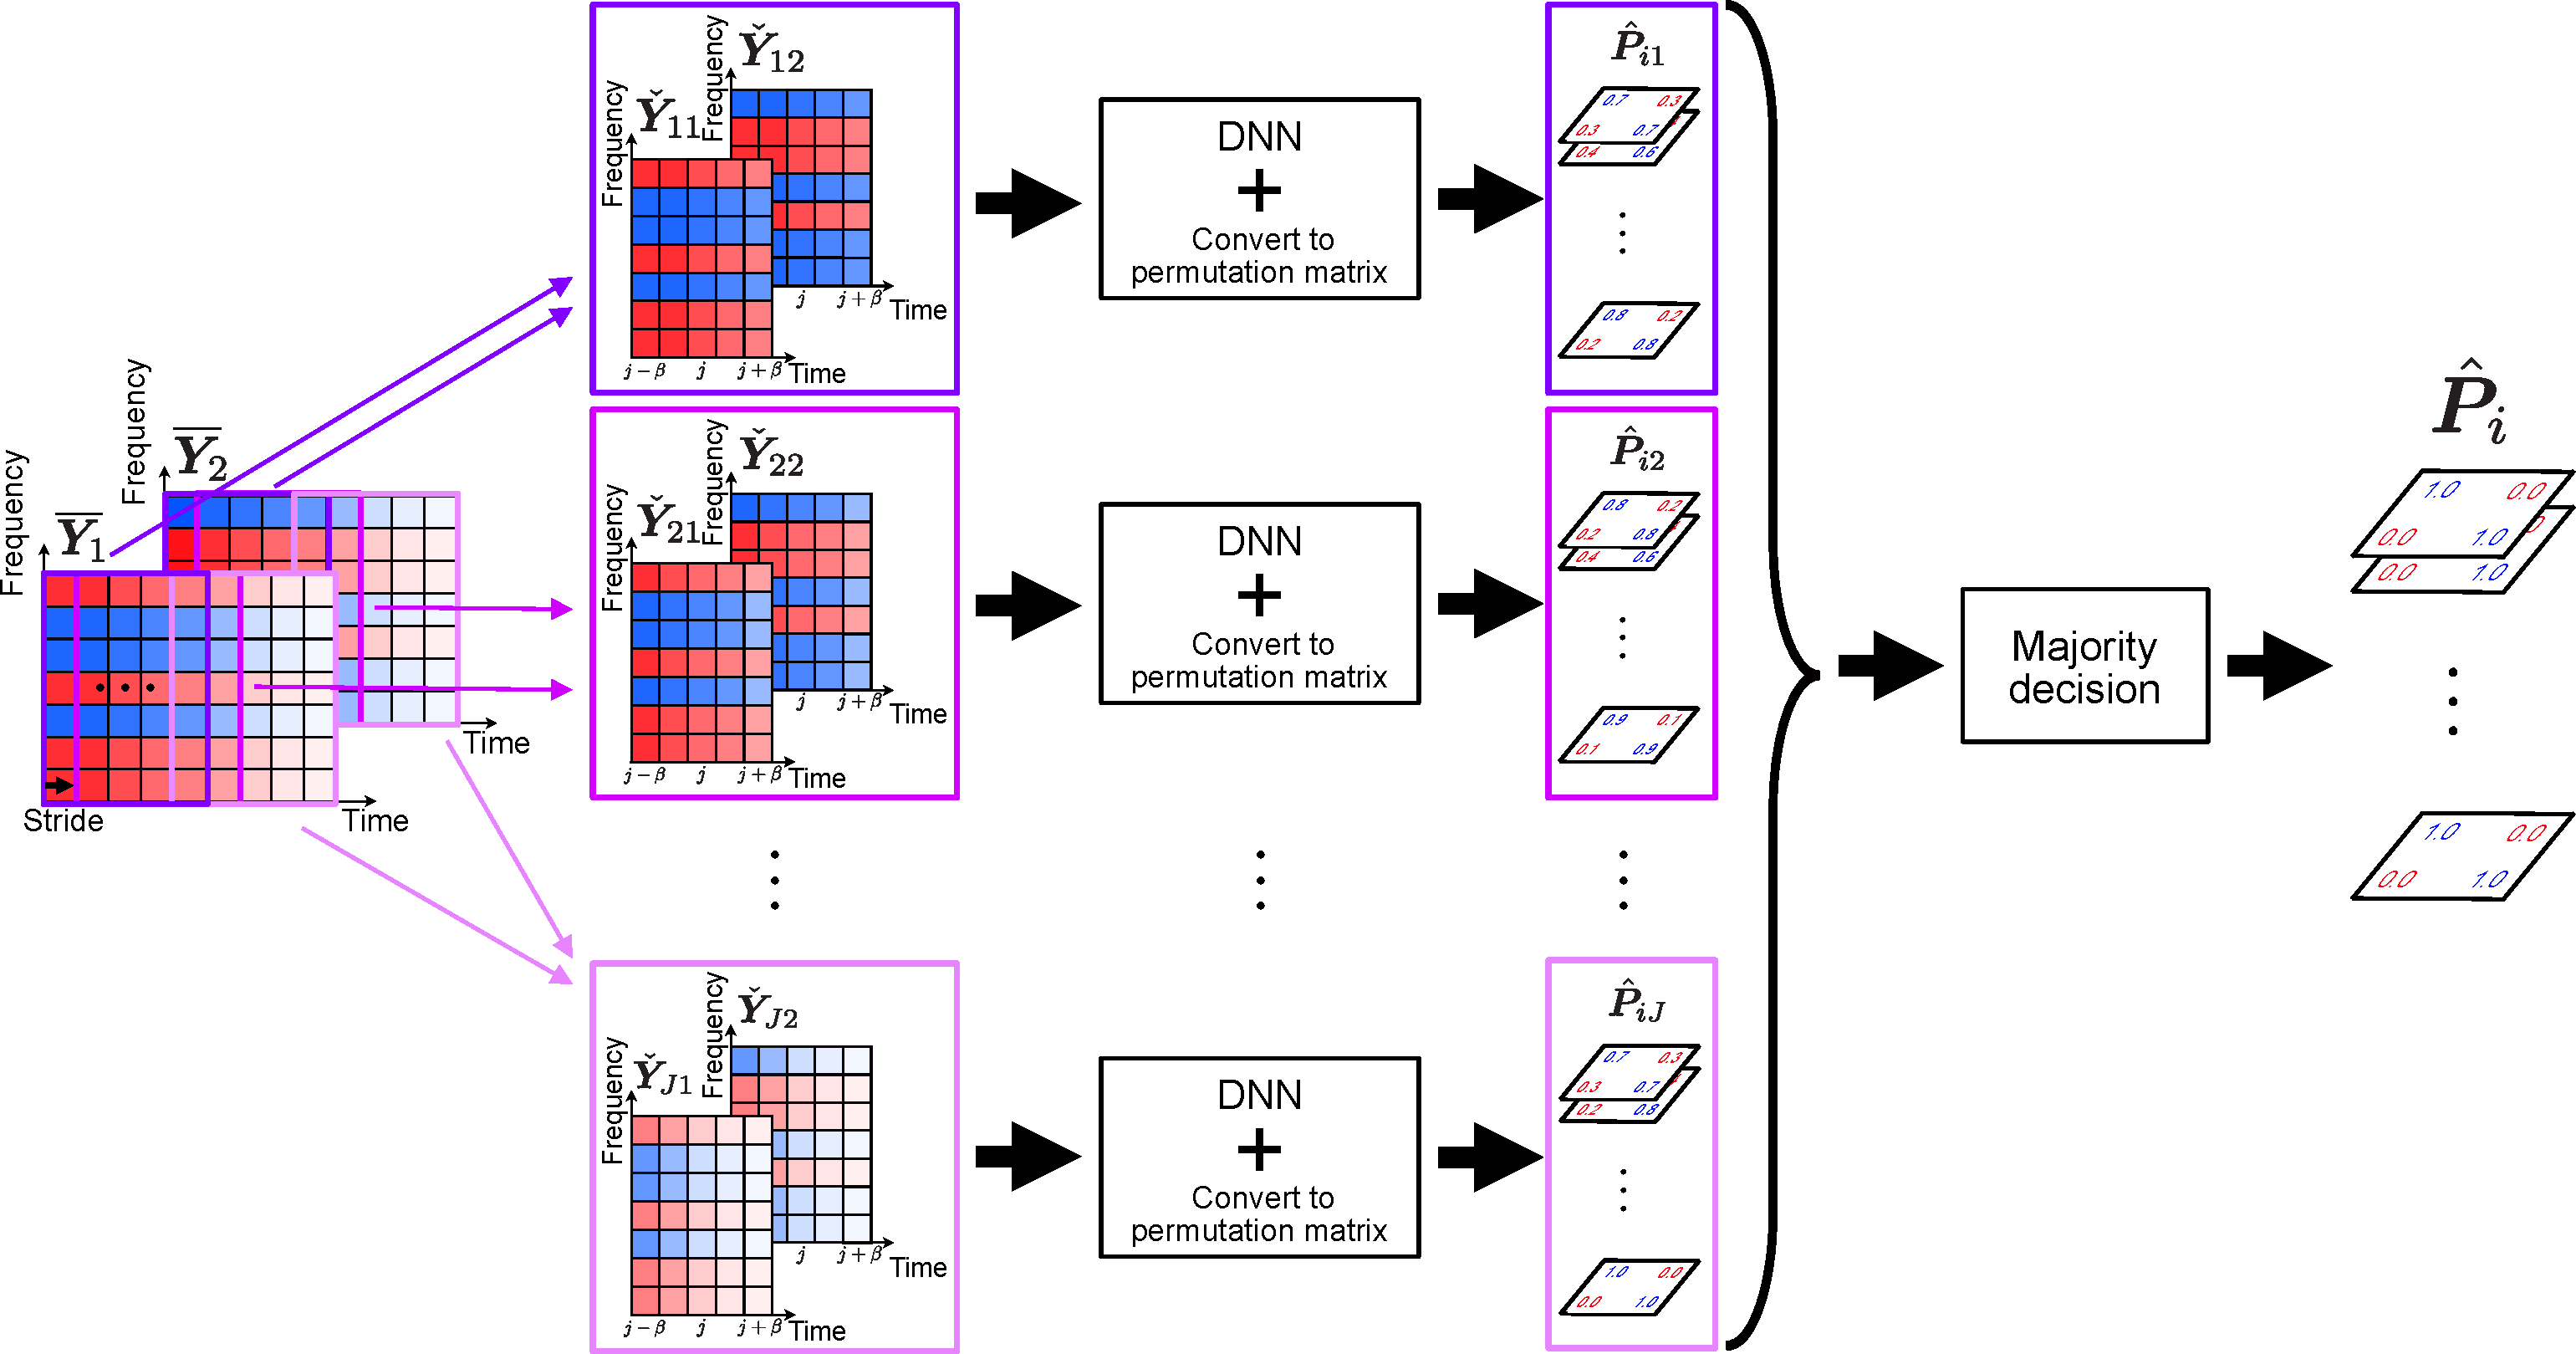
\includegraphics[width=1.0\columnwidth]{figures/majority.pdf}
    \end{center}
    \vspace{-15pt}
	\caption{DNN predictions for all local-time-frame amplitude \red{spectrograms} and their majority decision.}
	\label{fig:majority}
	\vspace{-8pt}   % キャプションと本文の間隔微調整用クトル
\end{figure}
%%%%%%%%%%%%%%%%%%%%%%%%%%%%
\blue{音声信号は本来,無音区間が多く存在することから,一定区間の長さの成分を持つ{$\widehat{\bm{Y}}_1$や$\widehat{\bm{Y}}_2$}はほぼ零ベクトルになる可能性があり,その場合DNNの予測は不安定になる.}
\blue{この問題に対処するために,Fig.~{\ref{fig:majority}}に示すように,長さ{$2\tau+1$}の入力ベクトルをストライド幅1でシフトさせて,全時間フレームに対してDNNの予測処理を走査する.}
\red{DNN学習後は,提案手法である深層パーミュテーション解決法をFDICA等の推定信号$(\bm{Y}_1, \bm{Y}_2)$に適用することができる.
このテストデータへの適用時においては,より高精度にパーミュテーション問題を解決をするために,次に示す2つの処理を施す.
\begin{enumerate}
\renewcommand{\labelenumi}{(\alph{enumi})}
  \item FDICA等で実現される周波数ビン毎のBSSが完全に達成されているならば,推定すべきパーミュテーション行列$\bm{P}_i$は0及び1の要素を持つバイナリ行列であるため,推定局所時間パーミュテーション行列$\hat{\bm{P}}_{ij}$もバイナリ行列に変換する
  \item FDICA等の時不変な分離行列$\bm{W}_i$を推定するBSSにより生じるパーミュテーション問題は,時間フレーム方向には一定である($\bm{P}_i$は$j$に非依存)ため,推定局所時間パーミュテーション行列$\hat{\bm{P}}_{ij}$を時間方向に多数決処理し,時不変な行列$\hat{\bm{P}}_{i}$に変換する
\end{enumerate}}

\red{上記(a)については,次式でバイナリ行列への変換処理を実現する.
\begin{align}
  \hat{\bm{P}}_{ij} \leftarrow \mathrm{round}( \hat{\bm{P}_{ij}} ) \in \{ 0, 1 \}^{N\times N} \label{eq:binarization}
\end{align}
ここで,$\mathrm{round}(\cdot)$は入力された行列の各要素に関して四捨五入を適用する処理であり,また$\leftarrow$は変数の更新を表す.
但し,式\eqref{eq:binarization}によるバイナリ行列への変換は,前段の周波数ビン毎のBSSが完全に達成されていることを仮定している.
実際にはFDICAでも周波数ビン毎のBSSには誤差が生じるため,式\eqref{eq:binarization}を適用すべきか否かは前段のBSSの性能に依存して決める必要がある.
本論文では,次章の実験条件で述べる通り,前段のBSSが完全であることを仮定しているため,式\eqref{eq:binarization}の処理を適用している.}
\blue{そして,DNNの予測結果を時間軸に関して多数決することで,より信頼性の高いラベル{$\widehat{\bm{L}}$}を得る.
この処理は,次のように示される.}

一方,上記(b)については,純粋にパーミュテーション問題の解決精度の向上に寄与する処理である.
DNNに入力する局所時間振幅スペクトログラム$(\check{\bm{Y}}_{1j}, \check{\bm{Y}}_{2j})$は推定信号$(\bm{Y}_1, \bm{Y}_2)$の各時間フレームにおいて抽出できるため,
Fig.~\ref{fig:majority}に示すように$(\check{\bm{Y}}_{1j}, \check{\bm{Y}}_{2j})$の抽出範囲をストライドさせ,その全てである$( (\check{\bm{Y}}_{1j}, \check{\bm{Y}}_{2j}) )_{j=1}^J$を個々にDNNに入力し,
全ての予測結果$( (\widehat{\check{\bm{Z}}}_{1j}, \widehat{\check{\bm{Z}}}_{2j}) )_{j=1}^J$を得ることができる.これらの予測結果を推定パーミュテーション行列$( \hat{\bm{P}}_{ij} )_{j=1}^J$に変換し,次式の多数決処理を適用する.
\begin{align}
  \hat{\bm{P}}_{i} = \mathrm{round}\left( \frac{1}{J} \sum_{j=1}^J \hat{\bm{P}}_{ij} \right) \label{eq:majorityDecision}
\end{align}
\red{なお,式\eqref{eq:binarization}のバイナリ行列への変換を適用しない場合においても,式\eqref{eq:majorityDecision}を計算することで時間方向の平均化ができるため,式\eqref{eq:majorityDecision}は上記(a)の適用の有無にかかわらず計算することが望ましい.}

%----------------------------------------------
\section{本章のまとめ}
\label{sec:3matome}
%----------------------------------------------
本章では,FDICAのポスト処理としてDNNに基づくパーミュテーション解決法について提案した.
\red{\ref{sec:moti}節では,FDICAにおいて理想的なパーミュテーション解決法を適用した場合,高精度で音源分離が可能となることを説明した.
\ref{sec:in-out}節では,DNNの入力に局所時間振幅スペクトログラムを用いることと,同一音源に属する成分の相関を強調させるため正規化を行うことを説明した.
\ref{sec:model}節では,隠れ層3層の全結合層からなるDNNの構造について説明した.
\ref{sec:loss}節では,DNNの予測に従ってパーミュテーション行列を作成した後,推定信号を並び替えた予測分離信号と正解の分離信号との間で損失を取得することを説明した.
\ref{sec:maj}節では,テストデータに対して時間方向に多数決処理を行うことで,パーミュテーション問題の解決精度を向上させることを説明した.}
\blue{提案手法は,各音源のパワースペクトログラムに対して全ての分離信号のパワースペクトログラムで割ったものをDNNの入力として用いる.また,DNNの出力である確率値を用いてパーミュテーション行列を並び替え,
後に完全に分離されたスペクトログラムとの間でMSEを行うことと,時間方向への多数決処理を用いることで,より精度の高い予測ができる.}


%%%%% 第4章 %%%%%
\chapter{実験}
\label{chap:ex}

%----------------------------------------------
\section{まえがき}
%----------------------------------------------
前章で提案したDNNに基づくパーミュテーション解決法の有効性を確認するために,人工的に作成したデータと実際の音声及び音楽信号を用意し,提案パーミュテーション解決法を適用する.後に,その性能を評価した.
\ref{sec:ex_condition}節では,本実験における条件を詳細に示し,\ref{sec:ex_res}節では提案手法のパーミュテーション解決性能を示している.
\ref{sec:matome}節で本章のまとめを述べる.
%----------------------------------------------
\section{実験条件}
\label{sec:ex_condition}
%----------------------------------------------
% \begin{table}[t]
% \begin{center}
%  \caption{Experimental conditions}
%  \label{table:ex}
%   \begin{tabular}{clll}\hline \hline
%    Window function in STFT & Hamming window  \\ \hline
%    Window length in STFT & 512~ms  \\ \hline
%    Shift length in STFT & 128~ms \\ \hline
%    Paramaters in Adam optimizer & \begin{tabular}{c}
%    \begin{flushleft}Learning rate = $0.001$\end{flushleft}\\
%    \begin{flushleft}$\beta = 0.9$\end{flushleft}
%    \end{tabular}  \\ \hline 
%    Reverberation time & $T_{60} = 470$~ms\\ \hline
%    Source direction of training data & $(\theta_1, \theta_2)=(60^\circ, 120^\circ)$\\ \hline
%    Source direction of test data & \begin{tabular}{c}
%    \begin{flushleft}(\theta_1, \theta_2)=(60^\circ, 120^\circ)\end{flushleft}\\ 
%    \begin{flushleft}(\theta_1, \theta_2)=(60^\circ, 100^\circ)\end{flushleft}\\ 
%    \begin{flushleft}(\theta_1, \theta_2)=(70^\circ, 110^\circ)\end{flushleft}
%    \end{tabular}\\ \hline \hline
%   \end{tabular}
%  \end{center}
% \end{table}
本実験では,提案するDNNに基づくパーミュテーション解決法において,どの程度各周波数成分の並び替えができるかを実験的に確認した.
実験には,人工データと実際の音声及び音楽信号を用いた.
%----------------------------------------------
\subsection{人工データを用いた実験の条件}
\label{sec:ex_condition_matrix}
%----------------------------------------------
実験データとして,Fig.~\ref{fig:01mat_spec}--\ref{fig:stripe_spec}に示すように,全ての成分が0と1の行列,25列毎に0と1の値が入れ替わる行列,1列毎に0と1の値が入れ替わる行列の3パターンを使用した.
用意した3パターンの行列は,いずれもパーミュテーション問題が生じていない(完全に解決された状態の)分離信号$(\bm{Z}_1, \bm{Z}_2)$とみなして実験を行う.この時の行列のサイズは$I=J=100$とした.
また,ブロックパーミュテーションと呼ばれる,ブロック単位でのパーミュテーション問題を模擬するために,1行毎だけでなくFig.~\ref{fig:ex_block}のように2行,4行,8行毎に各周波数成分を音源間でランダムにシャッフルした行列を作成し,
これをパーミュテーション問題が生じている(未解決の)信号$(\bm{Y}_1, \bm{Y}_2)$の検証データ及びテストデータとみなして深層パーミュテーション解決法の入力に用いた際の性能を評価した.
学習データには,分離信号の局所時間振幅スペクトログラム$(\check{\bm{Z}}_1, \check{\bm{Z}}_2)$の周波数成分を指定した行数毎に音源間でランダムにシャッフルしたものを用いた.
Fig.~\ref{fig:stripe_spec}に示す1列毎に0と1の値が入れ替わる行列に対しては,Fig.~\ref{fig:1_5ratio_perm}に示すように,各周波数成分に対して5\%の割合で周波数$i$の成分と$i+1$の成分を同じ音源の成分にした場合と,
各周波数成分に対して1\%の割合で周波数$i$の成分と$i+1$の成分を同じ音源の成分にした場合の実験も行った.
この際,周波数が$I$の場合は,$I$と$I-1$の成分を同じ音源の成分とした.
DNNの最適化法にはAdam~\cite{adam}を用い,ハイパーパラメータはそれぞれ$\varepsilon=1.0\times10^{-8},~\beta_1 = 0.9,~\beta_2 = 0.999$及び,学習率$\eta=0.001$とした.
その他の学習パラメータについては,バッチサイズを8,エポック数を1000,学習に用いるシャッフルパターンを300として誤差逆伝搬による学習を行った.
客観評価尺度として,各周波数成分において正しく並び替えを行うことができた割合,即ち検証データに対する正答率を用いる.


%%%%%%%%%%%%%%%%%%%%%%%%%%%%
\begin{figure}[t]
  \begin{center}
      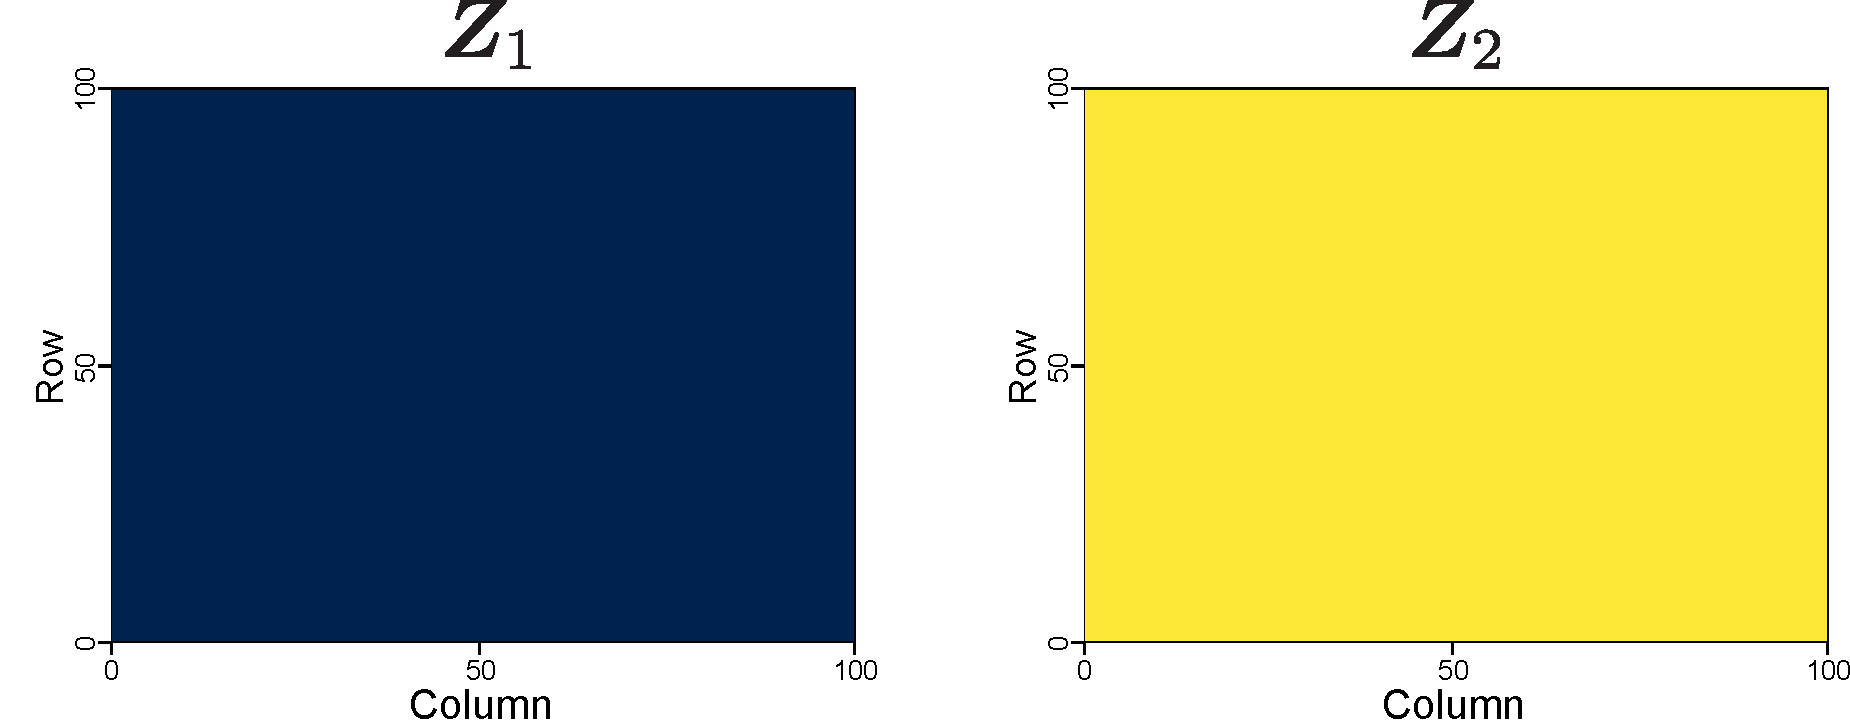
\includegraphics[width=0.95\columnwidth]{figures/origi_spec/01mat.pdf}
  \end{center}
\caption{Matrix with only 0 or 1 elements.}
\label{fig:01mat_spec}
\end{figure}
%%%%%%%%%%%%%%%%%%%%%%%%%%%%

%%%%%%%%%%%%%%%%%%%%%%%%%%%%
\begin{figure}[t]
  \begin{center}
      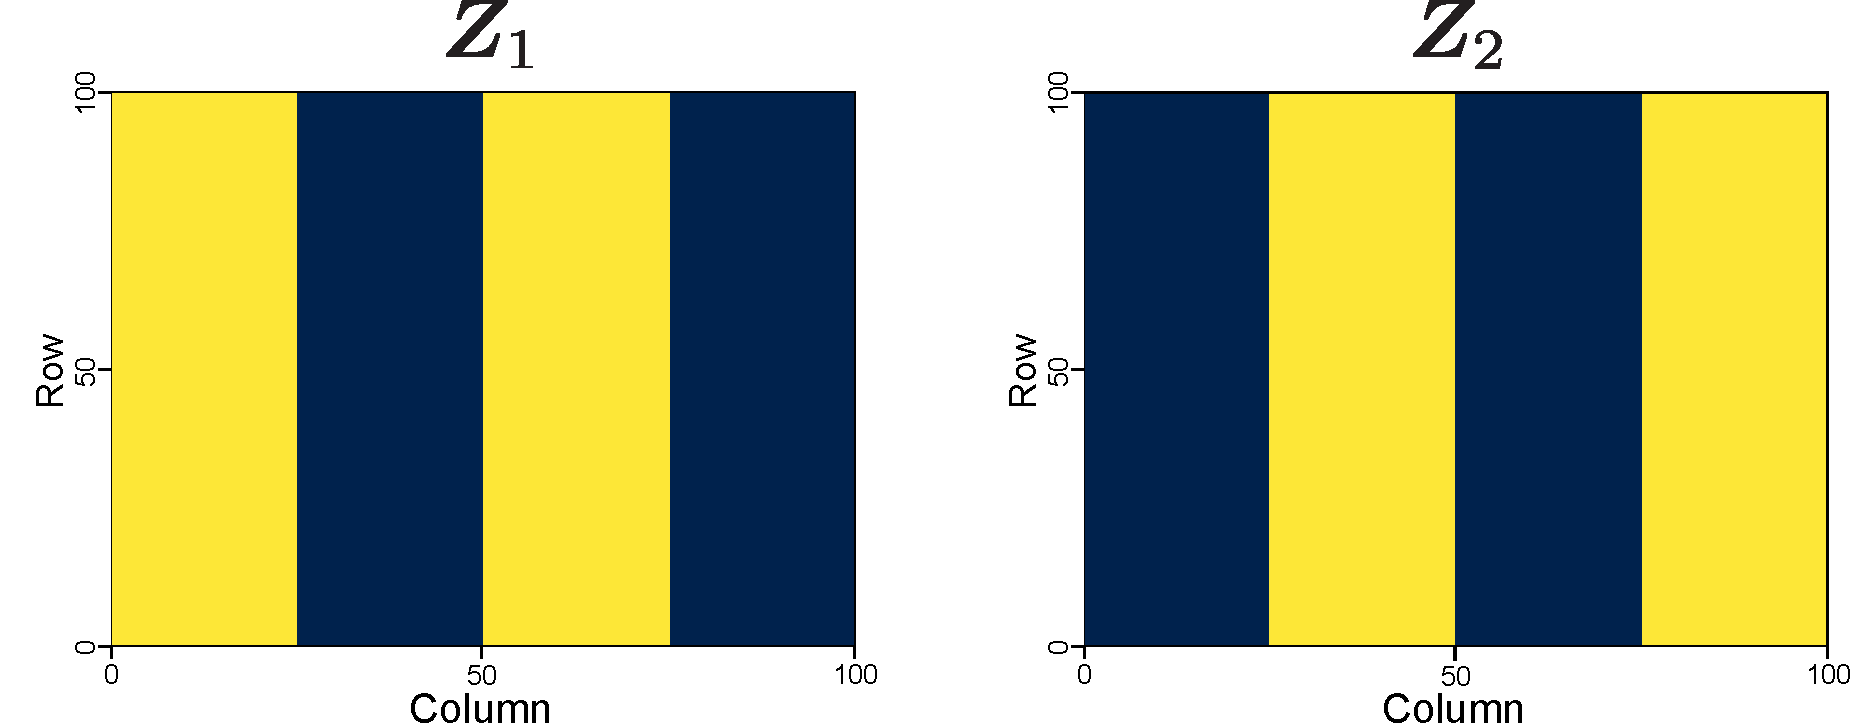
\includegraphics[width=0.95\columnwidth]{figures/origi_spec/25stripe.pdf}
  \end{center}
\caption{Two matrices with 0 and 1 values swapping every 25 columns.}
\label{fig:25stripe_spec}
\end{figure}
%%%%%%%%%%%%%%%%%%%%%%%%%%%%

%%%%%%%%%%%%%%%%%%%%%%%%%%%%
\begin{figure}[t]
  \begin{center}
      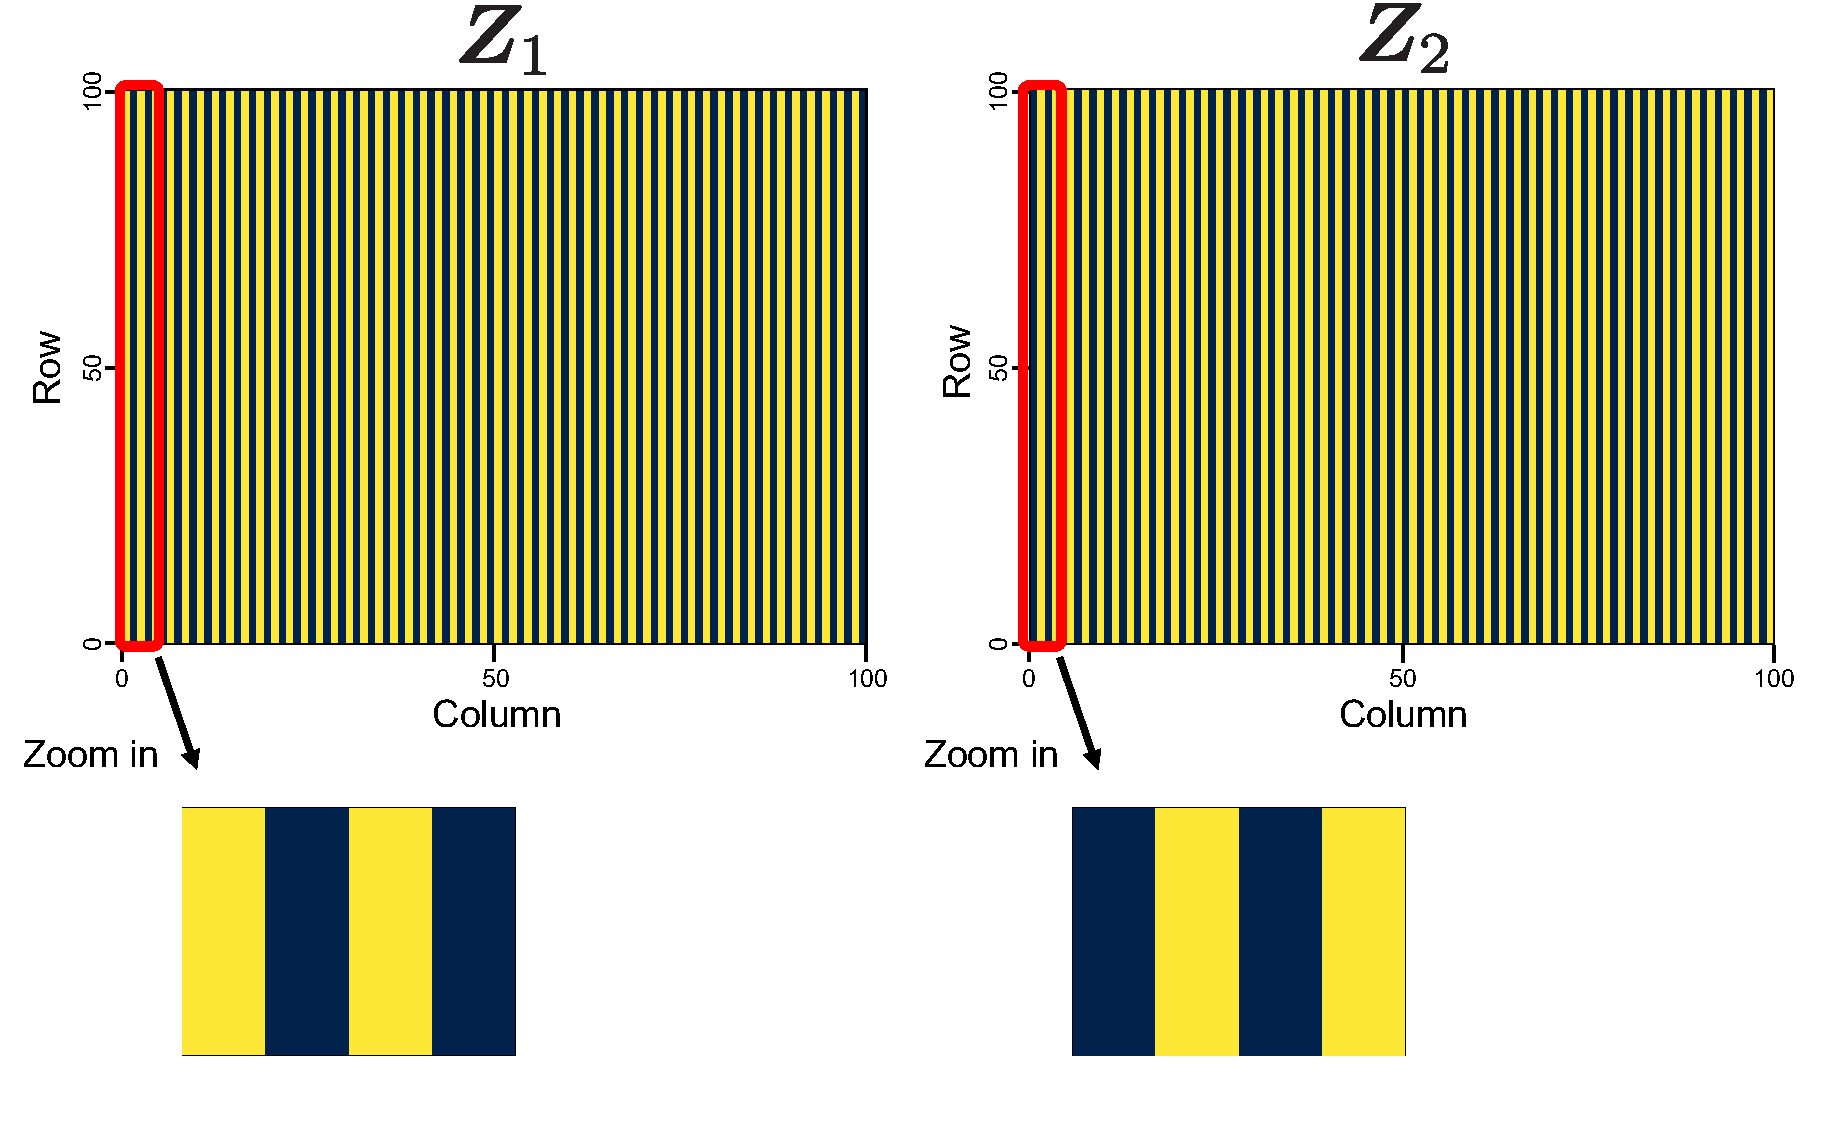
\includegraphics[width=0.95\columnwidth]{figures/origi_spec/stripe.pdf}
  \end{center}
\caption{Two matrices with 0 and 1 values swapping in each column.}
\label{fig:stripe_spec}
\end{figure}
%%%%%%%%%%%%%%%%%%%%%%%%%%%%

%%%%%%%%%%%%%%%%%%%%%%%%%%%%
\begin{figure}[t]
    \begin{center}
        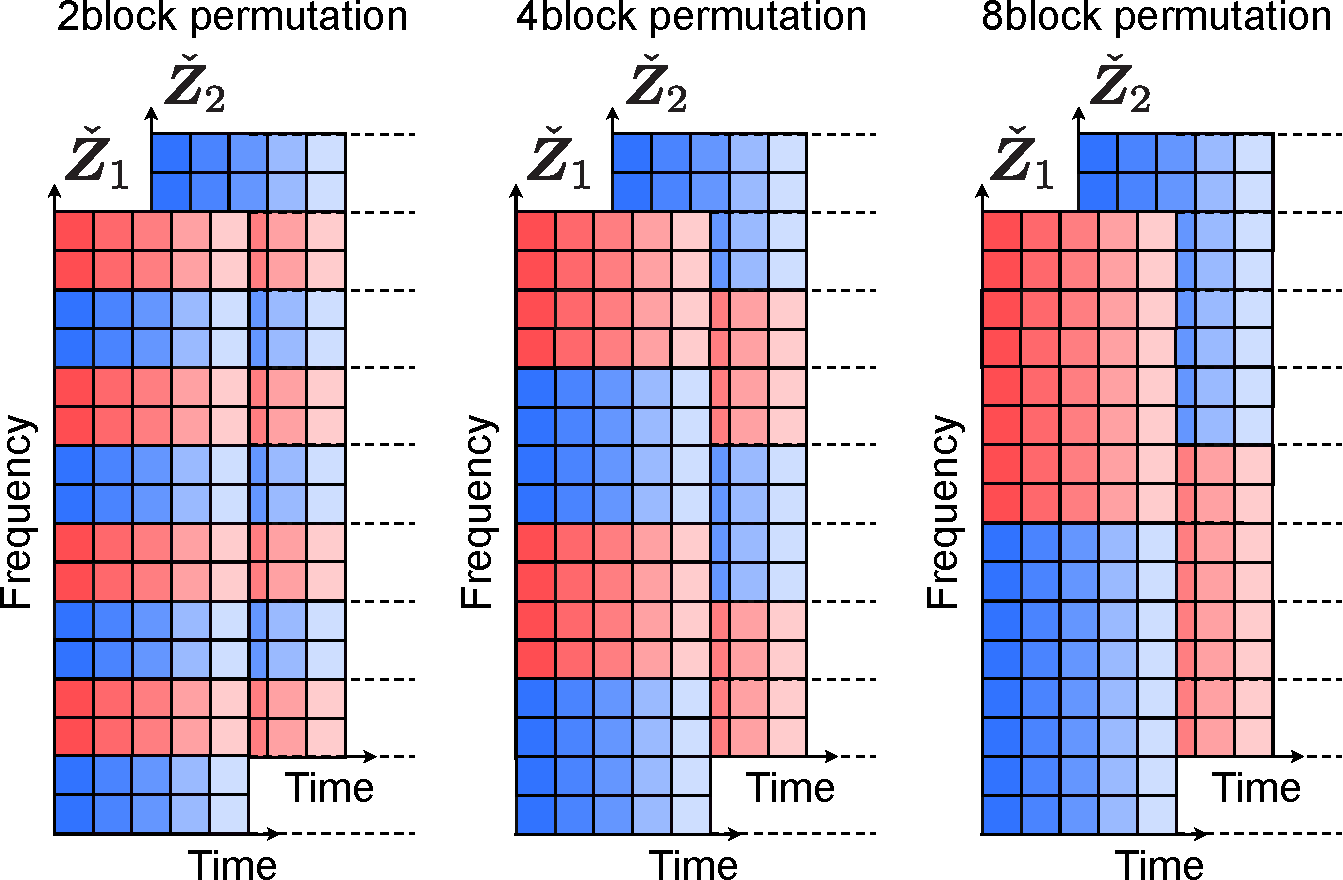
\includegraphics[width=1.0\columnwidth]{figures/experiment_block_matrix.pdf}
    \end{center}
	\caption{Example of block permutations used in the experiment.}
	\label{fig:ex_block}
\end{figure}
%%%%%%%%%%%%%%%%%%%%%%%%%%%%

%%%%%%%%%%%%%%%%%%%%%%%%%%%%
\begin{figure}[t]
    \begin{center}
        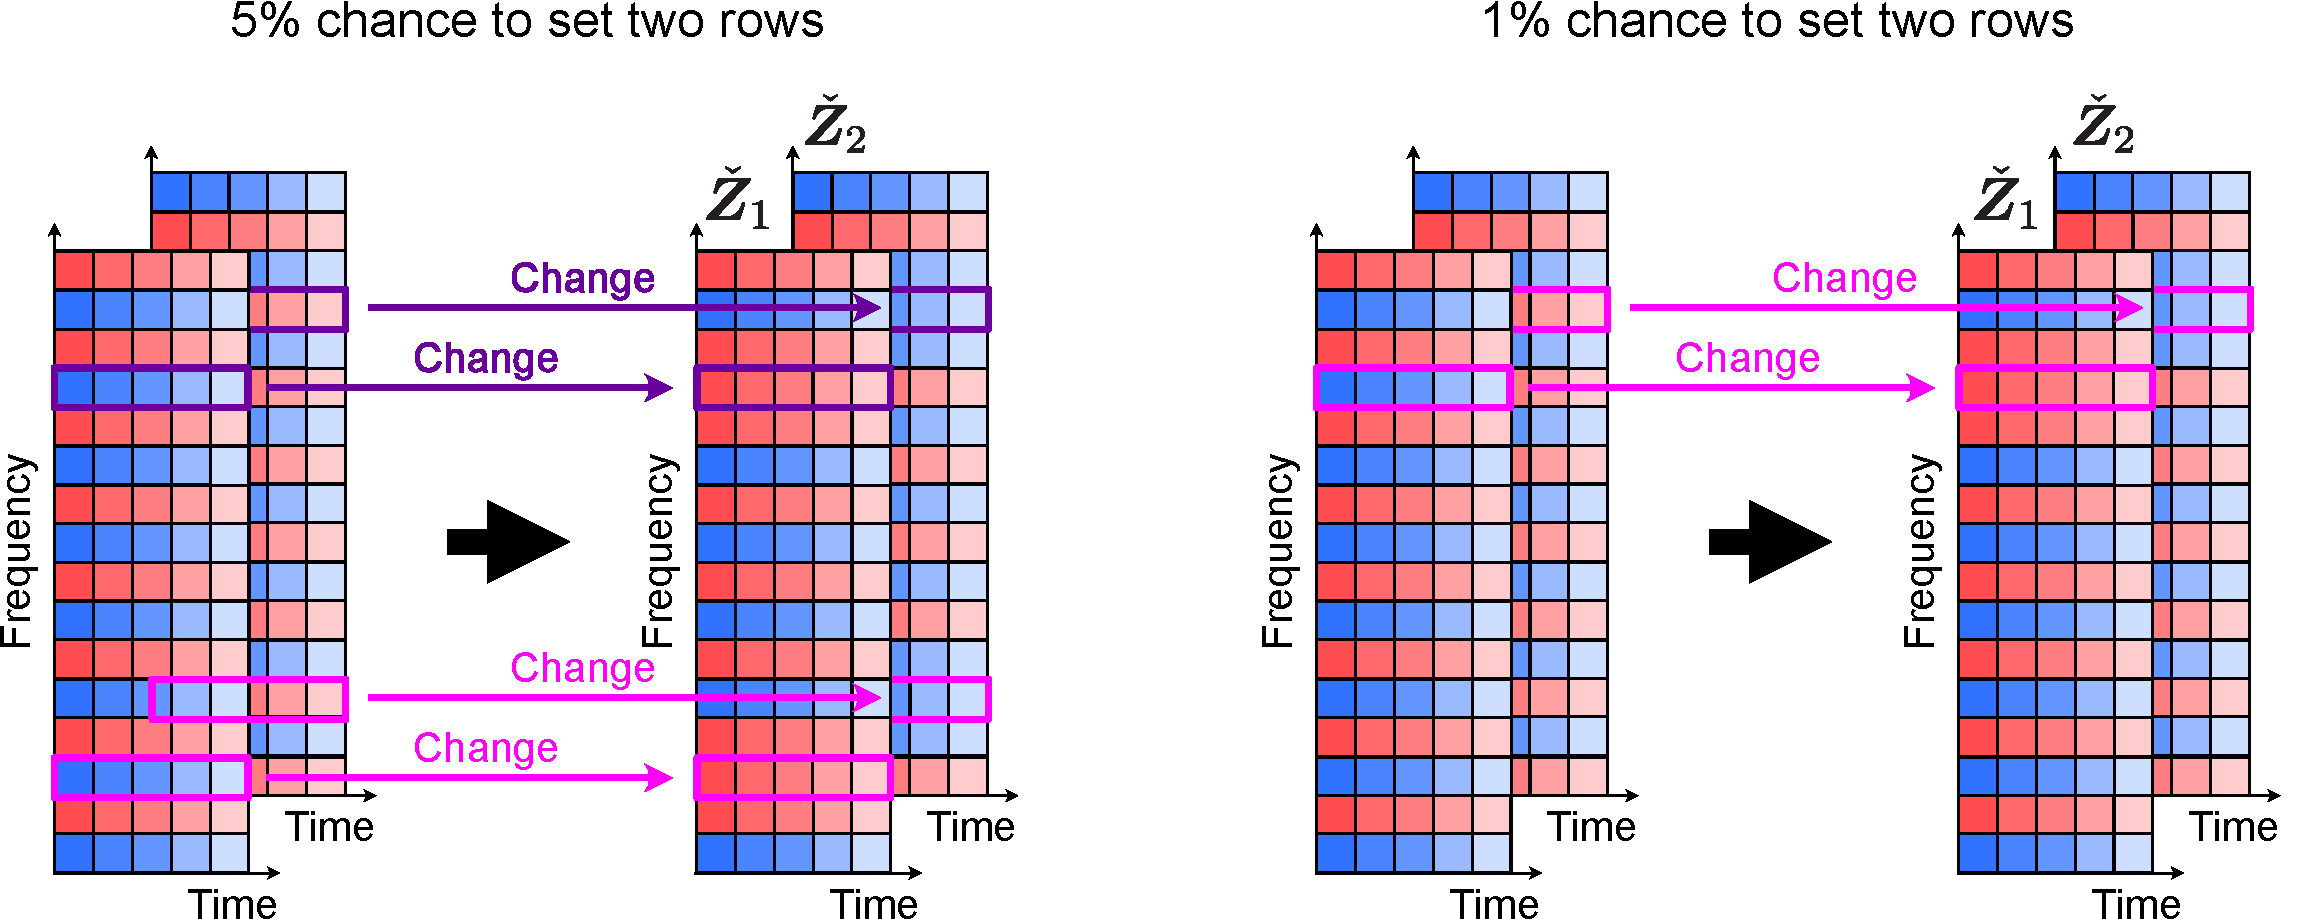
\includegraphics[width=1.0\columnwidth]{figures/1ratio_5ratio_permutation.pdf}
    \end{center}
	\caption{Shuffle the rows according to the specified percentage.}
	\label{fig:1_5ratio_perm}
\end{figure}
%%%%%%%%%%%%%%%%%%%%%%%%%%%%

\clearpage
%----------------------------------------------
\subsection{実際の音響信号を用いた実験の条件}
\label{sec:ex_condition_audio}
%----------------------------------------------

%----------------------------------------------
\begin{table}[t]
  \begin{center}
   \caption{Speech sources obtained from SiSEC2011}
   \label{table:wav}
    \begin{tabular}{clll}\hline \hline
     Signal  & Data name &Length~[s]  \\ \hline
     Speech  & dev3\_female4\_src\_2 & 10.0  \\ \hline
     Speech  & dev2\_male4\_src\_2 &  10.0 \\ \hline
     Piano   & dev2\_nodrums\_liverec\_250ms\_src\_3 & 11.0\\ \hline
     Drum   & dev2\_wdrums\_liverec\_250ms\_src\_3 & 11.0 \\ \hline 
     \hline
    \end{tabular}
   \end{center}
\end{table}
%%%%%%%%%%%%%%%%%%%%%%%%%%%%
\begin{figure}[t]
  \begin{center}
      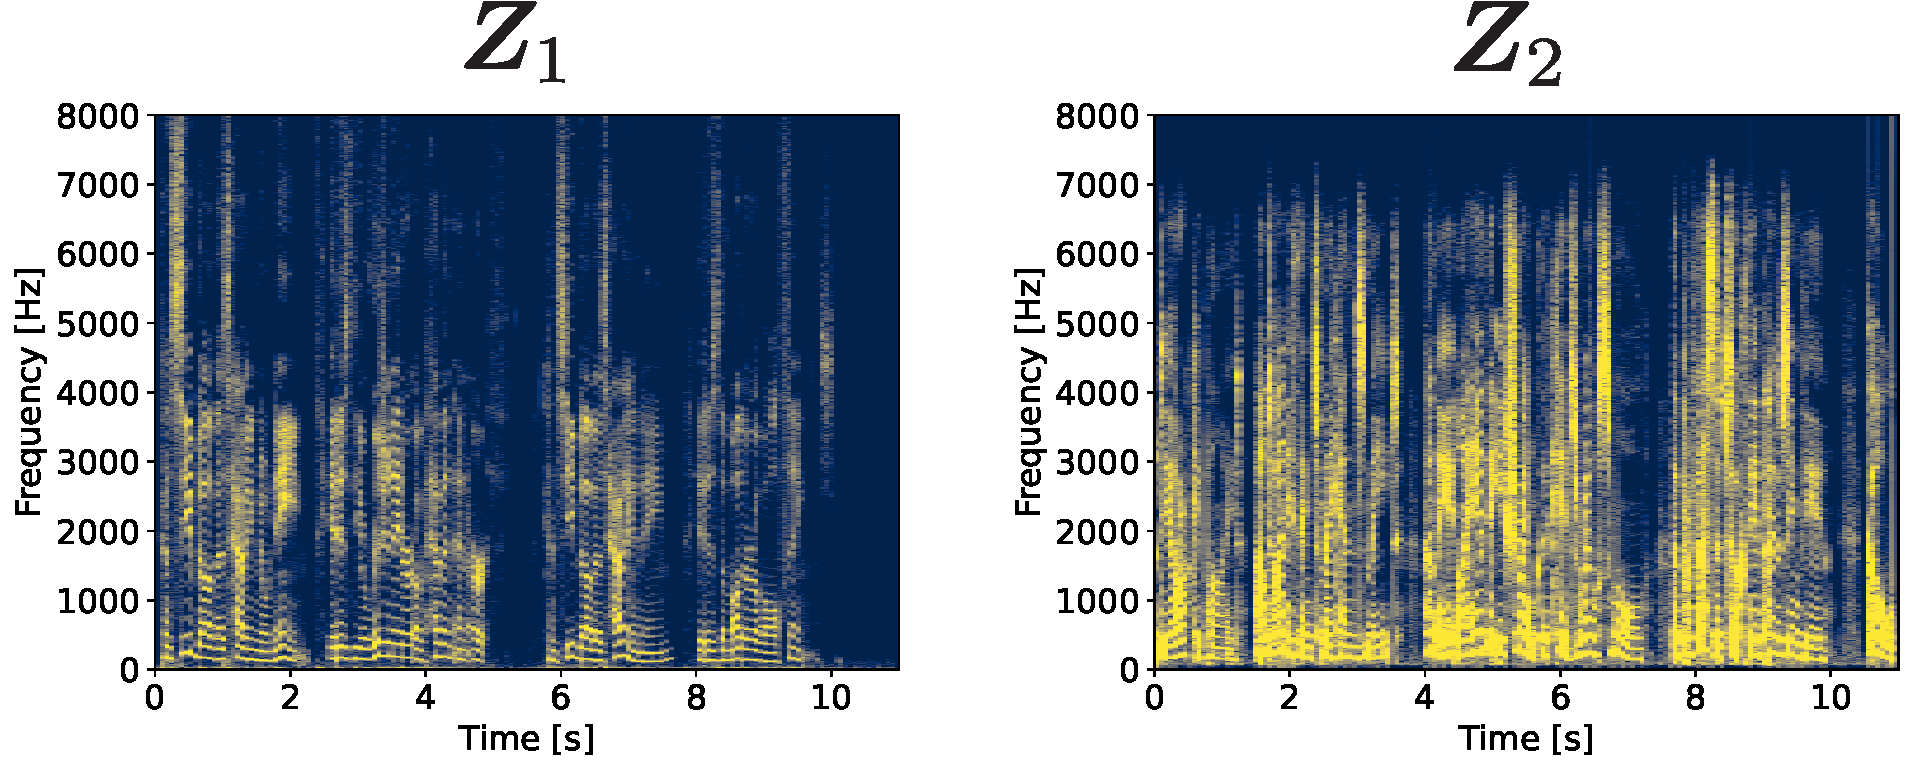
\includegraphics[width=0.95\columnwidth]{figures/audio_init_spec.pdf}
  \end{center}
\caption{Spectrograms of audio signal.}
\label{fig:audio}
\end{figure}
%%%%%%%%%%%%%%%%%%%%%%%%%%%%

%%%%%%%%%%%%%%%%%%%%%%%%%%%%
\begin{figure}[t]
  \begin{center}
      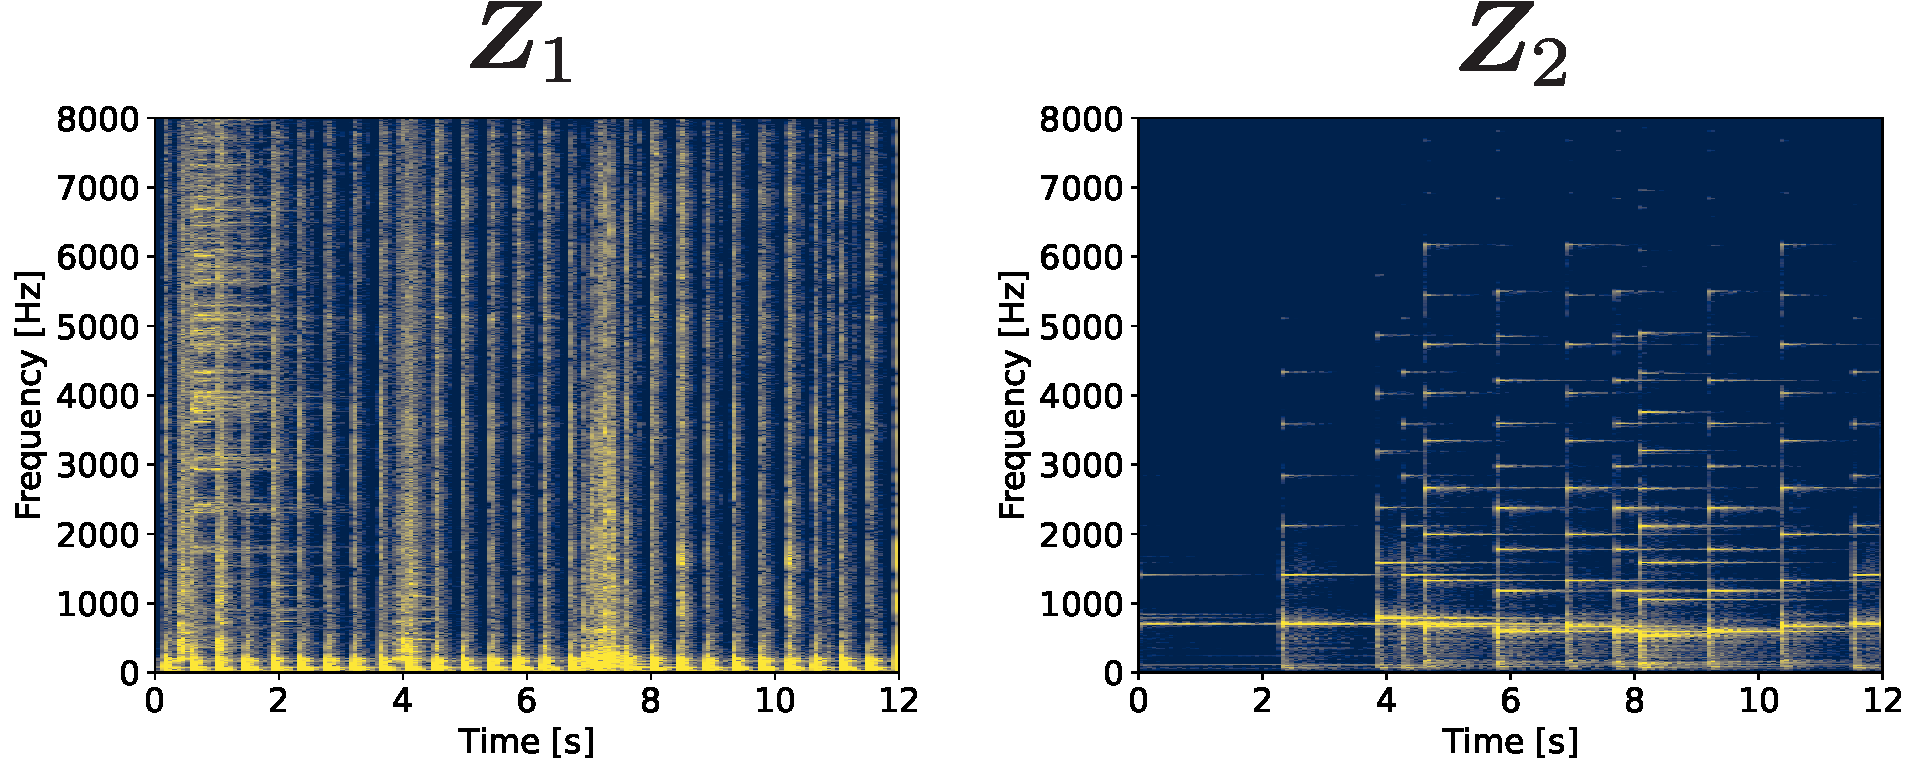
\includegraphics[width=0.95\columnwidth]{figures/Drum_init_spec.pdf}
  \end{center}
\caption{Spectrograms of music signal.}
\label{fig:drum}
\end{figure}
%%%%%%%%%%%%%%%%%%%%%%%%%%%%
%----------------------------------------------

実際の音響信号に対して提案手法がどの程度適用できるかを調べるために,Table~\ref{table:wav}に示すようにSiSEC2011~\cite{Sisec}の英語の音声信号(男性1名及び女性1名)2種類と楽器音(ピアノとドラム)2種類を使用した.
音声信号のスペクトログラムをFig.~\ref{fig:audio},楽器音のスペクトログラムをFig.~\ref{fig:drum}に示す.
音響信号に対するSTFTは,fftサイズ2048~ms,シフトサイズ1024~msに設定した.音声信号と楽器音の分離に対しては,ブロックパーミュテーション問題を解くことを想定し,16行毎に周波数成分をシャッフルした場合の実験を行った.
最適化法やハイパーパラメータについては,\ref{sec:ex_condition_matrix}項の条件と同じである.

実際の音響信号に対しては,検証データに対する正答率に加え,SDRの改善量を用いて提案手法の性能を評価する.
SDRは,音源分離の度合と分離音の歪みの少なさの両方を加味した客観指標である.
目的音を$\bm{s}(l)$,目的音以外の妨害音を$\bm{a}(l)$とすると,混合信号は以下のように表すことができる.
\begin{align}
    \bm{x}(l) = \bm{s}(l) + \bm{a}(l)
\end{align}
$\bm{x}(l)$に音源分離を適用し得られる目的音の推定信号$\bm{\hat{s}}(l)$は次式で表される.
\begin{align}
    \bm{\hat{s}}(l) = \bm{s}_{\mathrm{target}}(l) + \bm{e}_{\mathrm{interf}}(l) + \bm{e}_{\mathrm{artif}}(l)
\end{align}
ここで,$\bm{s}_{\mathrm{target}}(l),~\bm{e}_{\mathrm{interf}}(l),~\bm{e}_{\mathrm{artif}}(l)$はそれぞれ推定信号中の,目的音成分,残留した妨害音成分,及び音源分離である.
この時,SDRは次式のように算出できる.
\begin{align}
    \mathrm{SDR} = 10 \mathrm{log}_{10} \sum \frac{|\bm{s}_{\mathrm{target}}(l)|^2}{|\bm{e}_{\mathrm{interf}}(l) + \bm{e}_{\mathrm{artif}}(l)|^2}~~~\mathrm{[dB]}
\end{align}
%----------------------------------------------
\section{実験結果}
\label{sec:ex_res}
%----------------------------------------------
%----------------------------------------------
\subsection{人工データに対する実験結果}
\label{sec:ex_res_artificial}
%----------------------------------------------

Fig.~\ref{fig:01mat_1block}--\ref{fig:stripe_1block}には,全ての成分が0と1の行列,25列毎に0と1の値が入れ替わる行列,1列毎に0と1の値が入れ替わる行列の周波数成分に対して各周波数成分毎にシャッフルを行った場合の結果を示す.
この結果から,各周波数成分毎にシャッフルした場合,Fig.~\ref{fig:01mat_spec}やFig.~\ref{fig:25stripe_spec}に示すような,比較的簡易的な行列に対しては,それぞれ正答率が100\%に近い値となっている.
Fig.~\ref{fig:01mat_spec}とFig.~\ref{fig:25stripe_spec}の$\hat{\bm{Z}}_1$,$\hat{\bm{Z}}_2$は少しの間違いは含んでいるものの,高精度で並び替えができていることが分かる.
しかし,Fig.~\ref{fig:stripe_spec}に示すような,1列毎に0と1の値が入れ替わる行列に対して各周波数成分毎にシャッフルを行った場合は,Fig.~\ref{fig:stripe_1block}に示すように正答率が54\%程度となった.
$\hat{\bm{Z}}_1$,$\hat{\bm{Z}}_2$を見ても並び替えができていないことが分かる.
Fig.~\ref{fig:stripe_95ratio_1block}及びFig.~\ref{fig:stripe_99ratio_1block}は,各周波数成分に対して5\%の割合で周波数$i$の成分と$i+1$の成分を同じ音源の成分にした場合と,
各周波数成分に対して1\%の割合で周波数$i$の成分と$i+1$の成分を同じ音源の成分にした場合の実験結果を示す.
Fig.~\ref{fig:stripe_95ratio_1block}より,各周波数成分に対して5\%の割合で周波数$i$の成分と$i+1$の成分を同じ音源の成分にした場合の正答率は93\%程度となったが,
Fig.~\ref{fig:stripe_99ratio_1block}を見ると,各周波数成分に対して1\%の割合で周波数$i$の成分と$i+1$の成分を同じ音源の成分にした場合の正答率は60\%程度となった.
Fig.~\ref{fig:01mat_2block}--\ref{fig:stripe_2block}には,全ての成分が0と1の行列,25列毎に0と1の値が入れ替わる行列,1列毎に0と1の値が入れ替わる行列の周波数成分に対して2行毎にシャッフルを行った時の結果を示す.
Fig.~\ref{fig:01mat_2block}--\ref{fig:stripe_2block}に示すどの実験結果も検証データに対する正答率が90\%を超えており,推定分離信号$\hat{\bm{Z}}_1$,$\hat{\bm{Z}}_2$が完全分離信号に近い値となっていることが分かる.
即ち,DNNは少しでもブロック単位でシャッフルが行われていると学習が容易となり,高精度で分離信号を予測することが可能となることが分かる.
この他にも行列の周波数成分に対して4行毎と8行毎にシャッフルした時の実験を行なった.詳細は付録Bに掲載している.

%%%%%%%%%%%%%%%%%%%%%%%%%%%%
\begin{figure*}[!t]
    \centering
    \subfloat[Percentage of correct answers for training and validation data.]{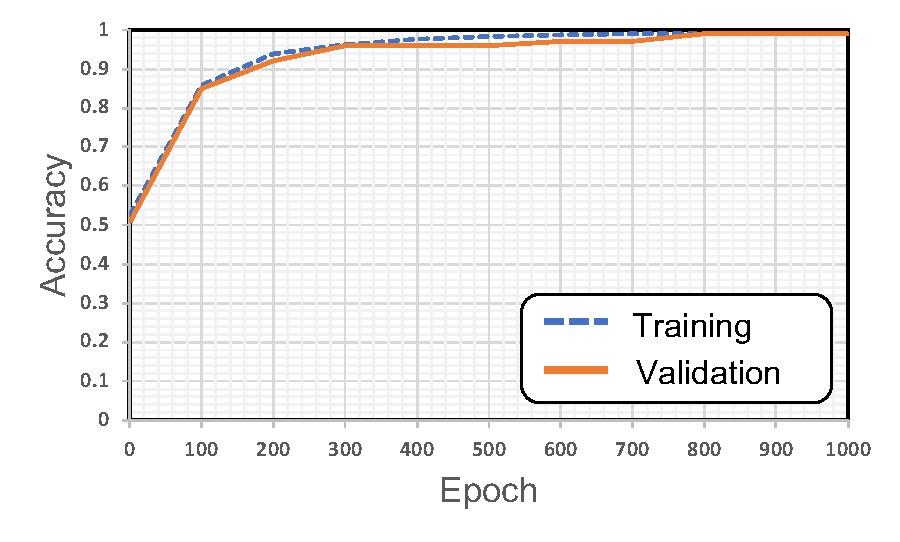
\includegraphics[clip, width=4.5in]{figures/01mat_1block_graph.pdf}
    \label{fig:acc_01mat_1block}}
    \\
    \subfloat[Spectrogram of estimated signal and predictive separation signal.]{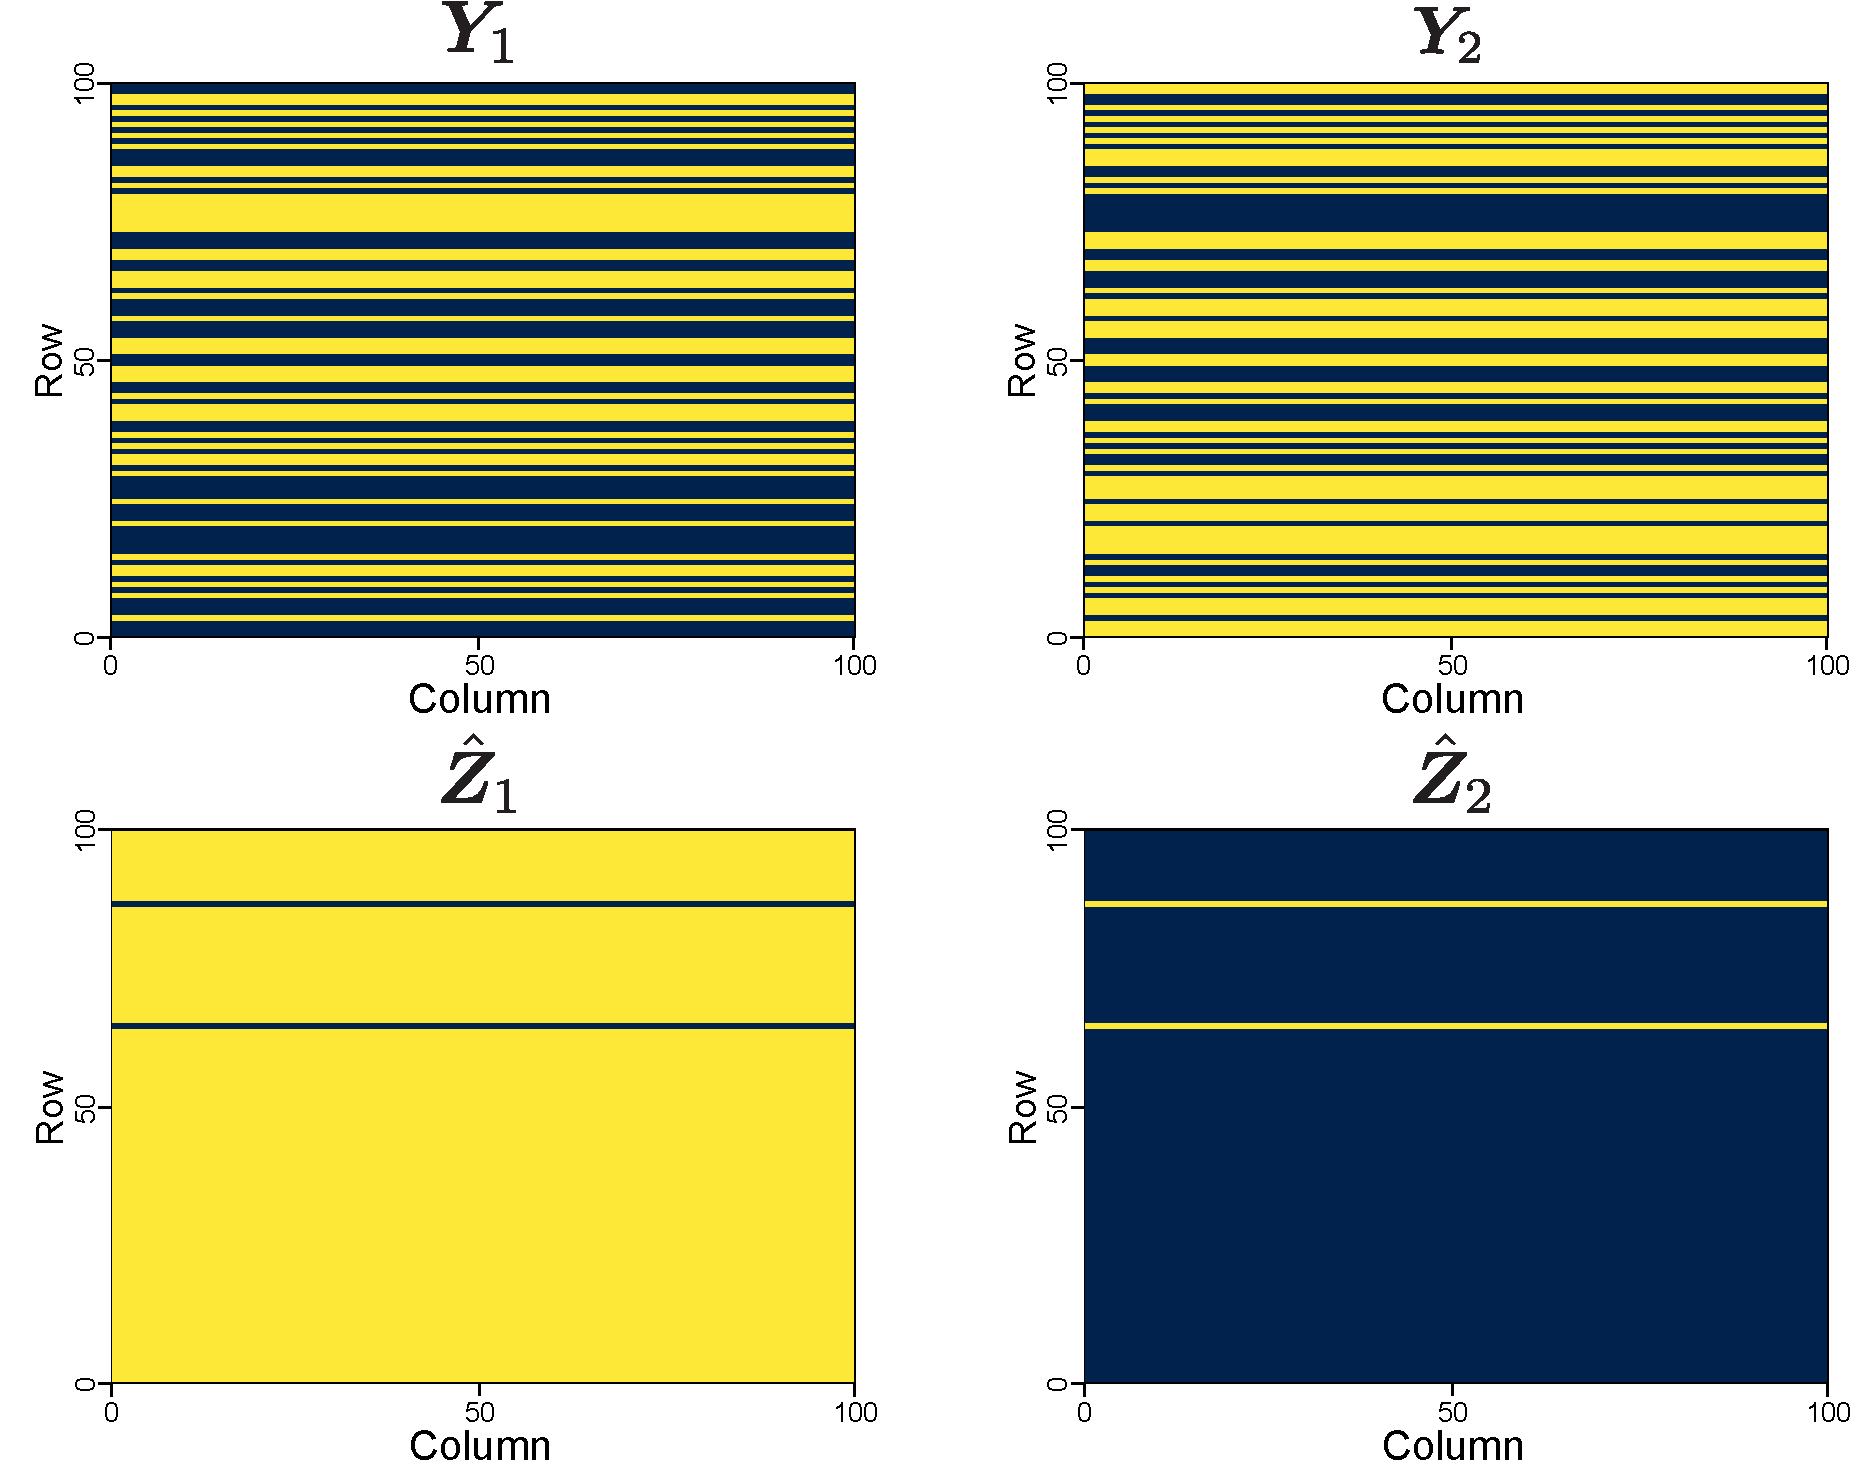
\includegraphics[clip, width=5.0in]{figures/01mat_1block.pdf}
    \label{fig:spec_01mat_1block}}  
    \caption{Experimental results using matrix of Fig~\ref{fig:01mat_spec} (randomly shuffle per row).}
    \label{fig:01mat_1block}
\end{figure*}
%%%%%%%%%%%%%%%%%%%%%%%%%%%%

%%%%%%%%%%%%%%%%%%%%%%%%%%%%
\begin{figure*}[!t]
    \centering
    \subfloat[Percentage of correct answers for training and validation data.]{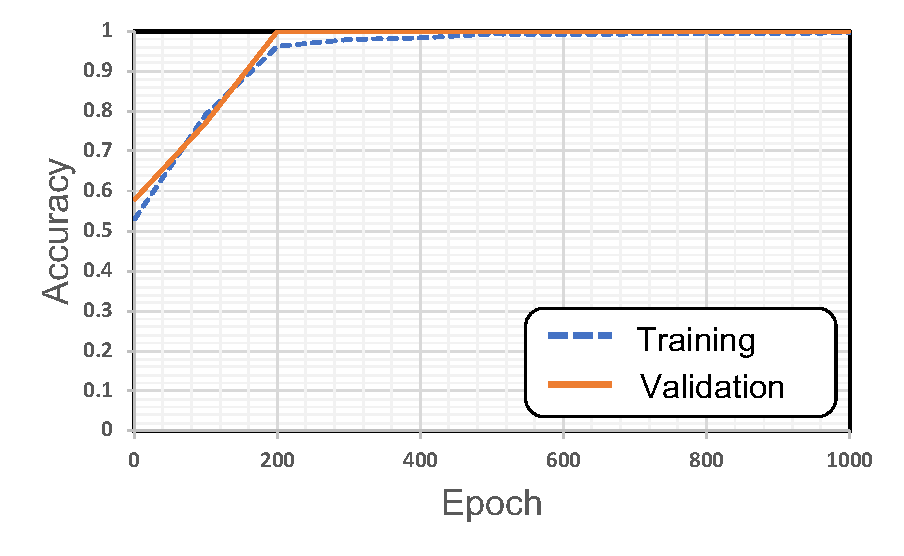
\includegraphics[clip, width=4.5in]{figures/graph_25stripe_1block.pdf}
    \label{fig:acc_25mat_1block}}
    \\
    \subfloat[Spectrogram of estimated signal and predictive separation signal.]{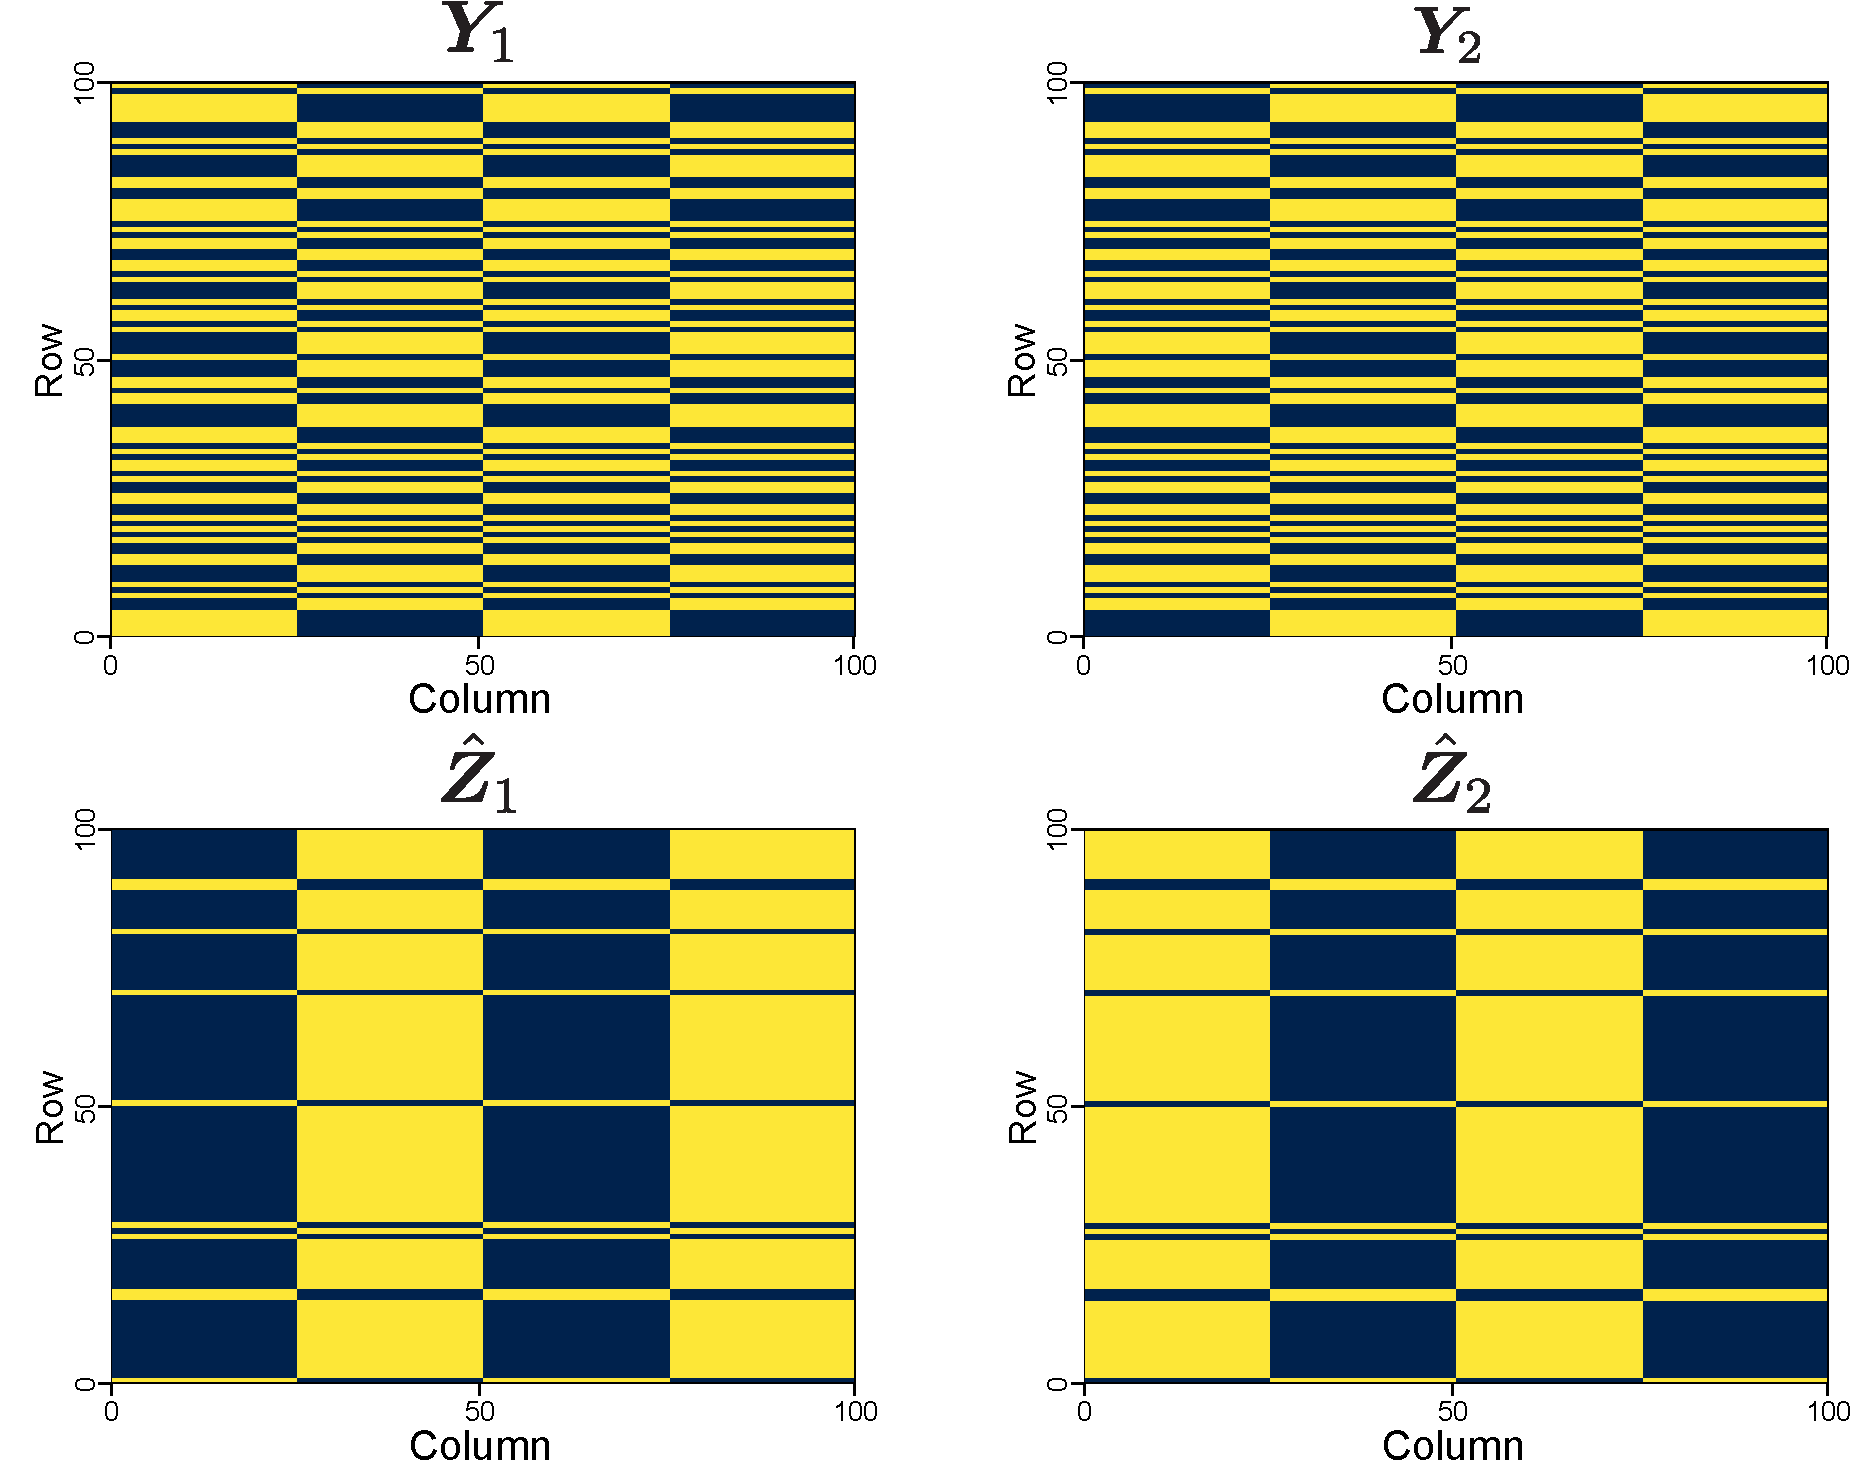
\includegraphics[clip, width=5.0in]{figures/25stripe_1block.pdf}
    \label{fig:spec_25mat_1block}}  
    \caption{Experimental results using the matrix of Fig~\ref{fig:25stripe_spec} (randomly shuffle per row).}
    \label{fig:25mat_1block}
\end{figure*}
%%%%%%%%%%%%%%%%%%%%%%%%%%%%

%%%%%%%%%%%%%%%%%%%%%%%%%%%%
\begin{figure*}[!t]
    \centering
    \subfloat[Percentage of correct answers for training and validation data.]{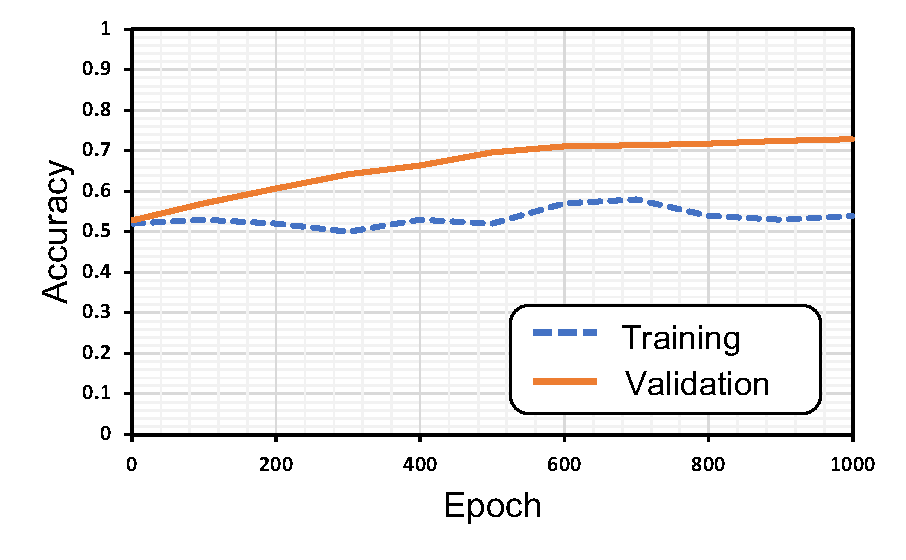
\includegraphics[clip, width=4.5in]{figures/graph/graph_stripe_1block.pdf}
    \label{fig:acc_stripe_1block}}
    \\
    \subfloat[Spectrogram of estimated signal and predictive separation signal.]{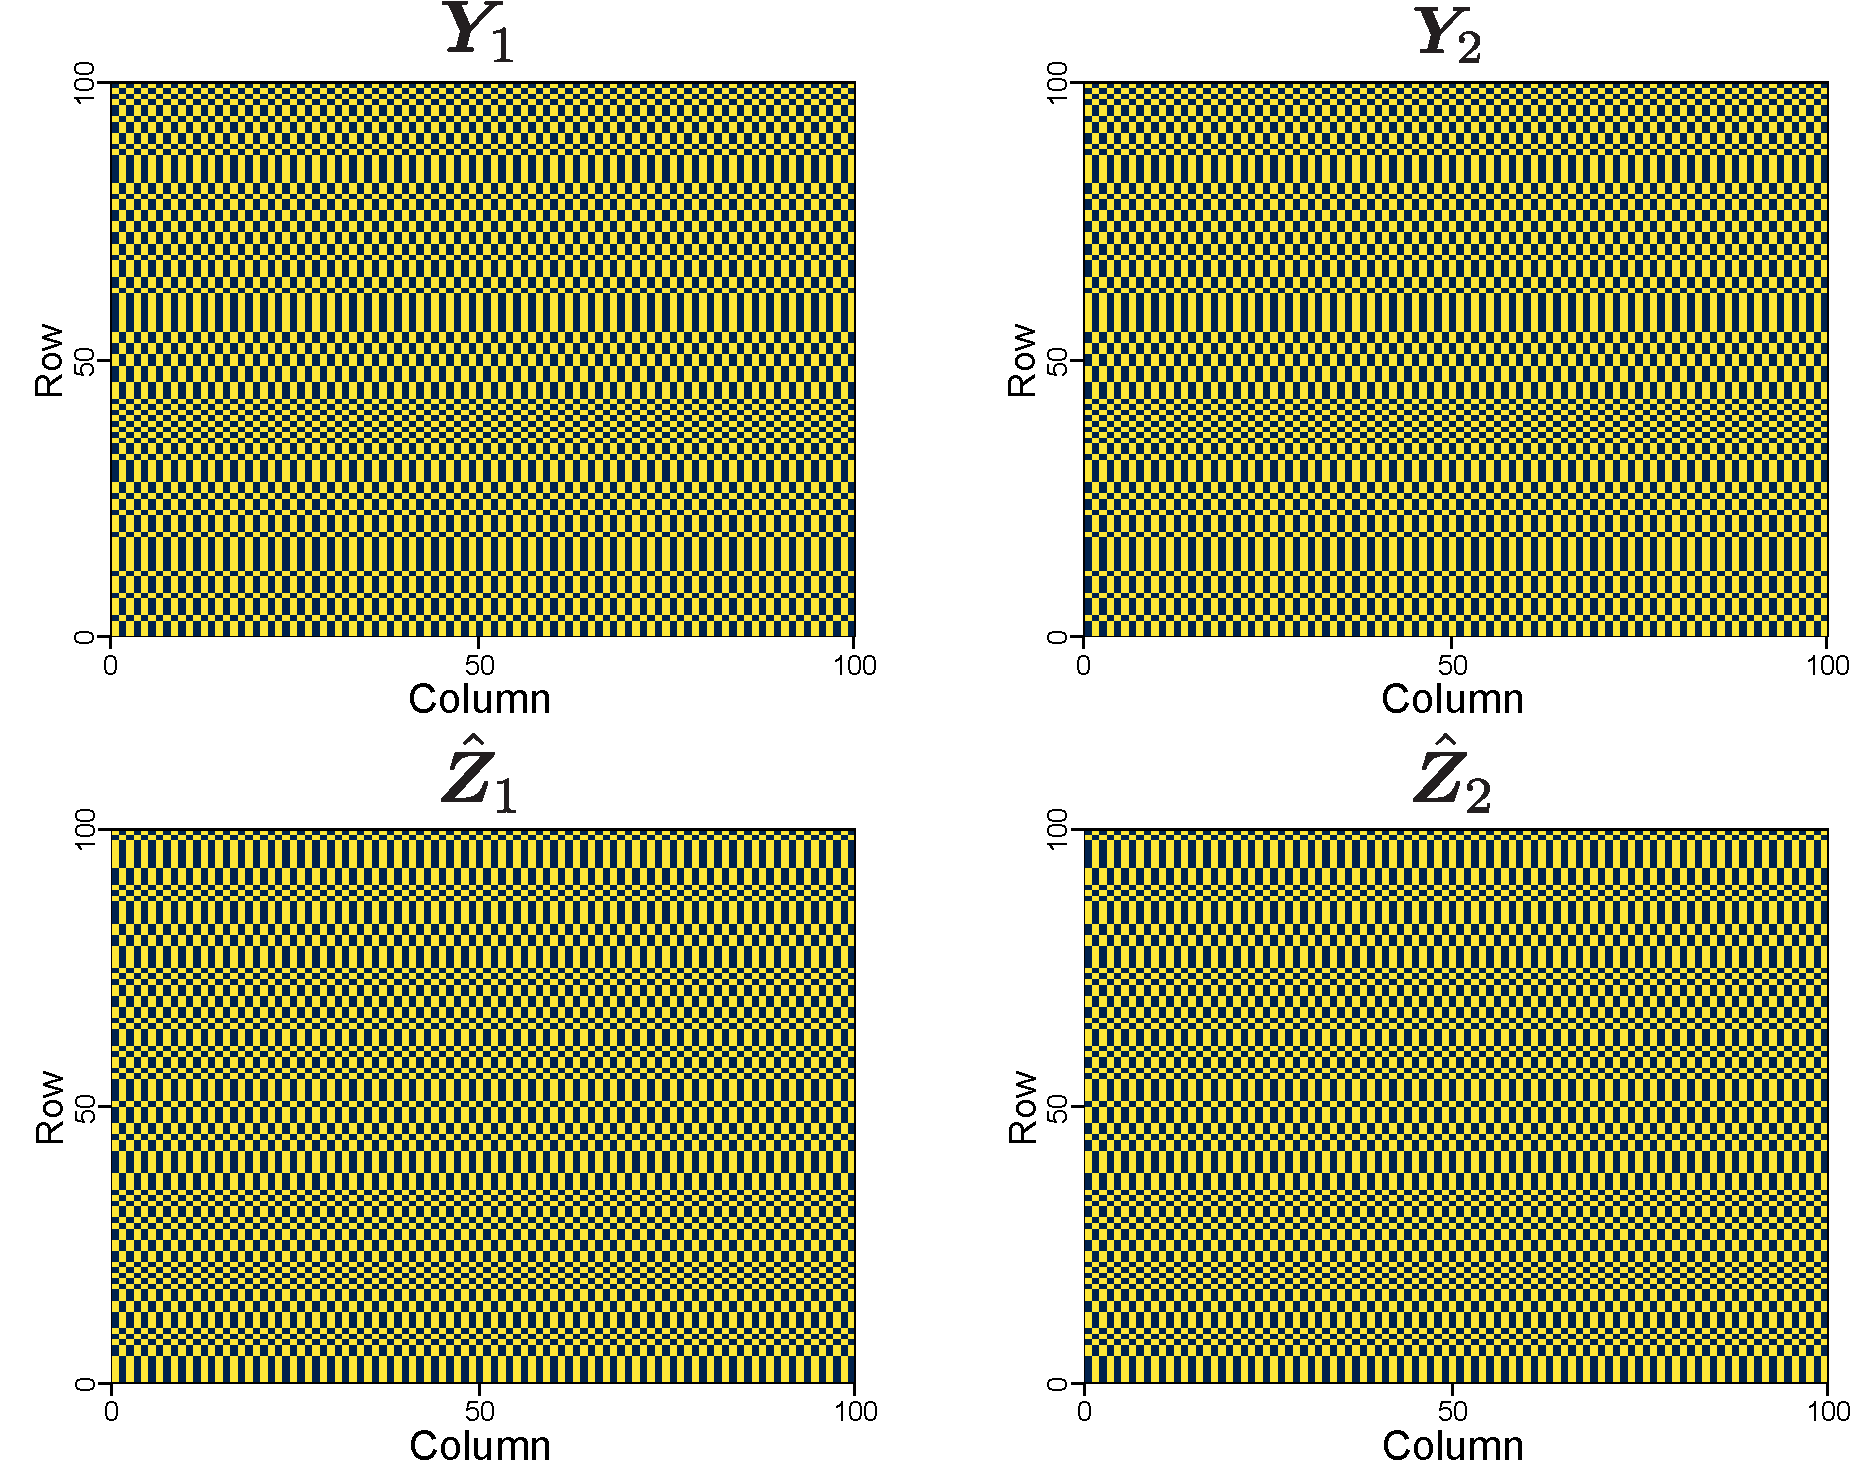
\includegraphics[clip, width=5.0in]{figures/stripe_1block.pdf}
    \label{fig:spec_stripe_1block}}  
    \caption{Experimental results using the matrix of Fig~\ref{fig:stripe_spec} (randomly shuffle per row).}
    \label{fig:stripe_1block}
\end{figure*}
%%%%%%%%%%%%%%%%%%%%%%%%%%%%

%%%%%%%%%%%%%%%%%%%%%%%%%%%%
\begin{figure*}[!t]
    \centering
    \subfloat[Percentage of correct answers for training and validation data.]{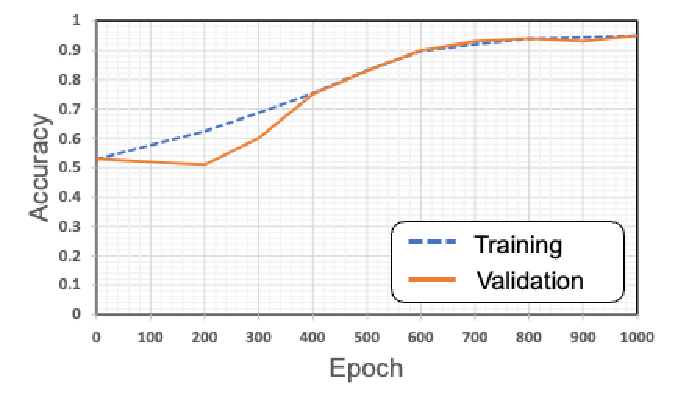
\includegraphics[clip, width=4.5in]{figures/graph_stripe_1block95ratio.pdf}
    \label{fig:acc_stripe_95ratio_1block}}
    \\
    \subfloat[Spectrogram of estimated signal and predictive separation signal.]{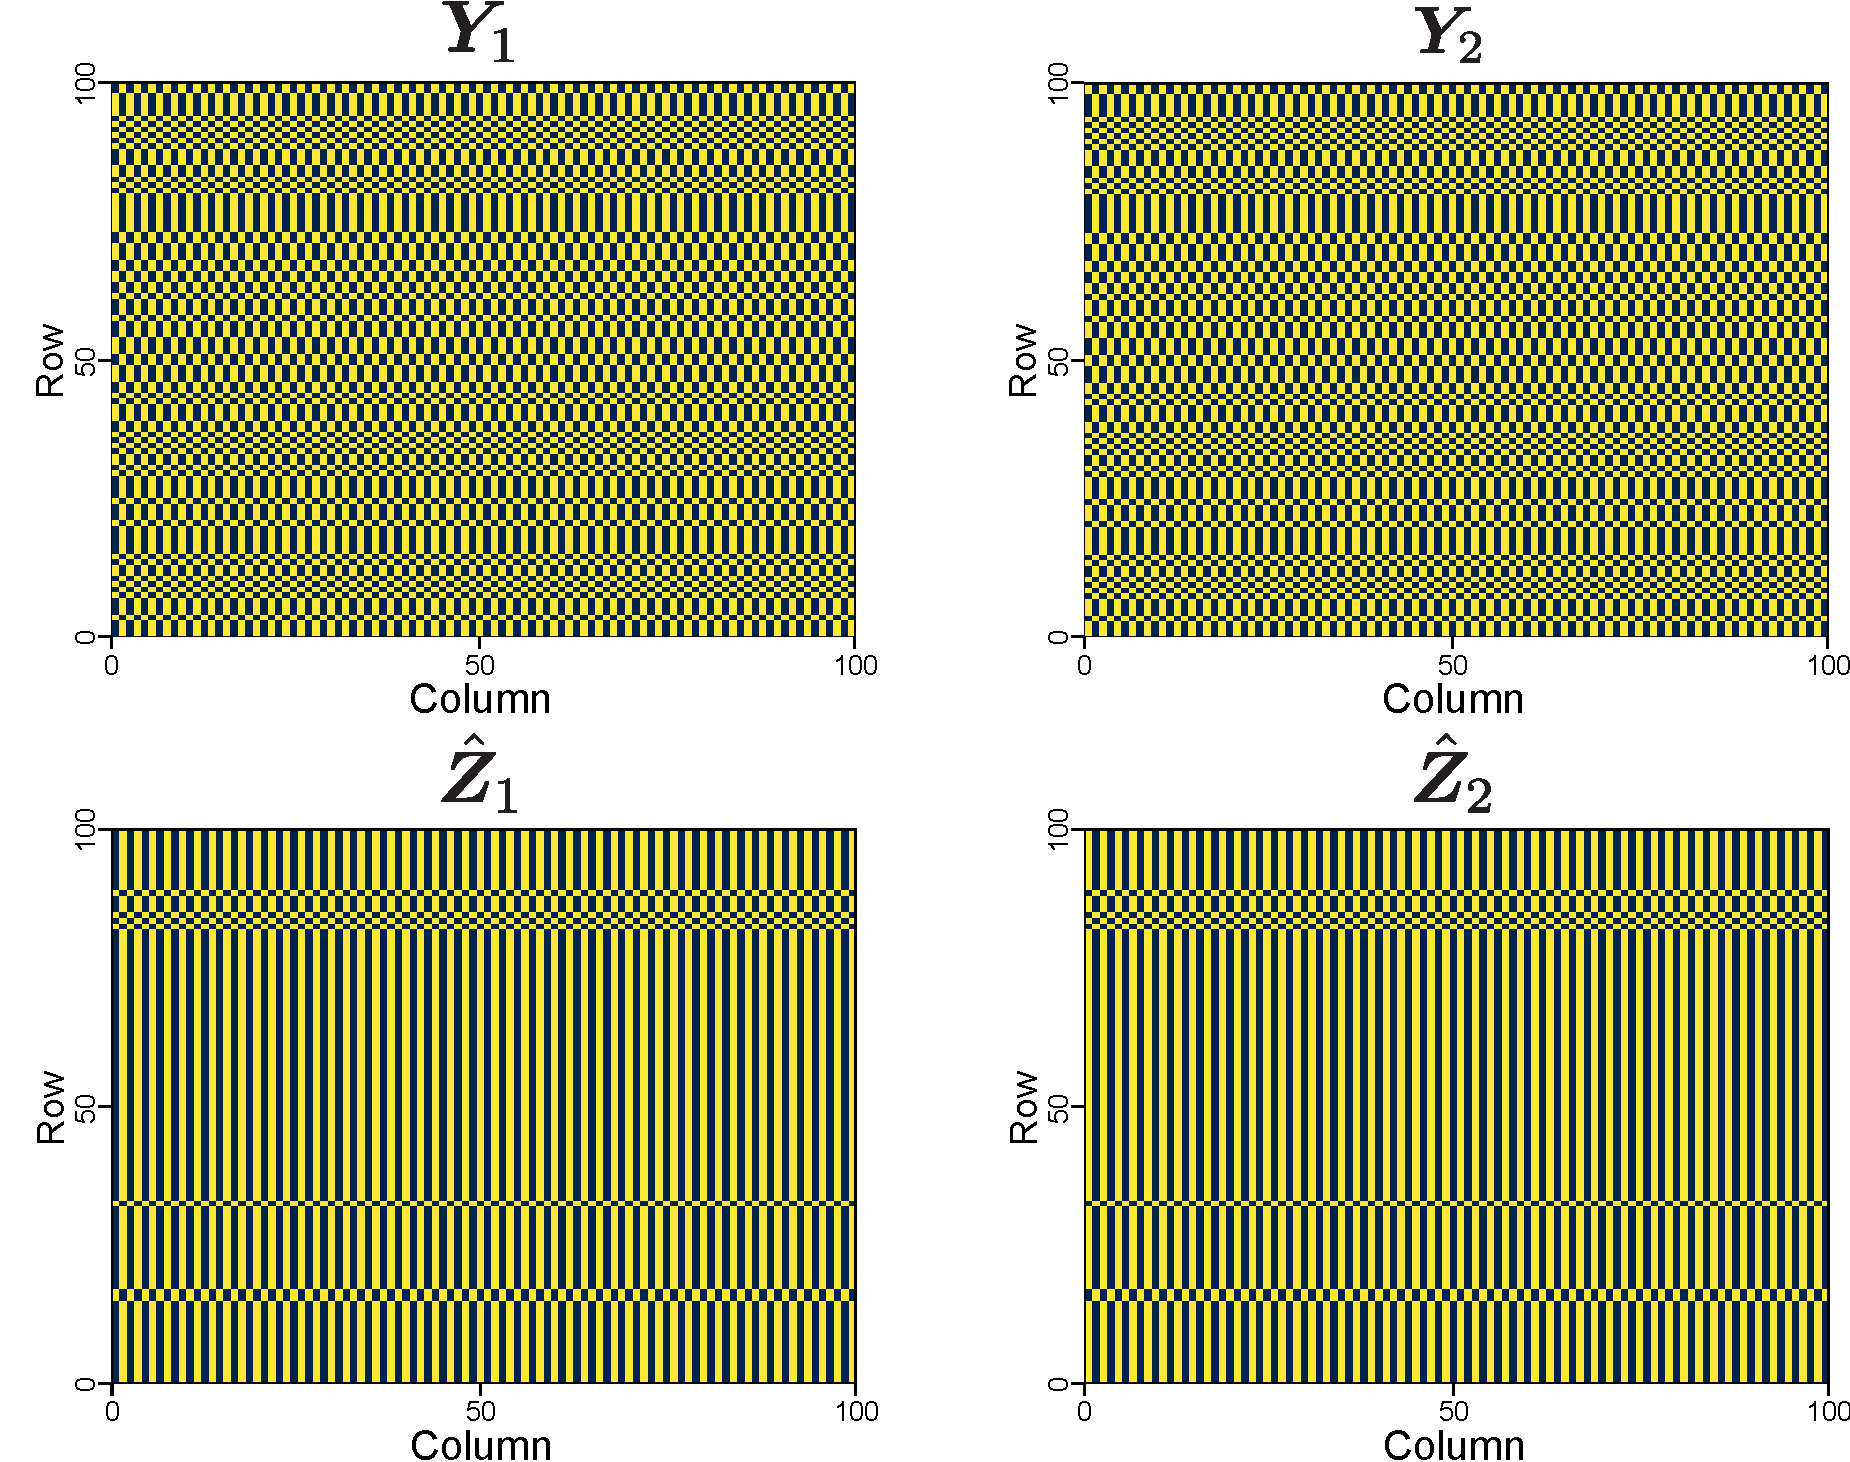
\includegraphics[clip, width=5.0in]{figures/stripe95ratio_1block_spec.pdf}
    \label{fig:spec_stripe_95ratio_1block}}  
    \caption{Experimental results using the matrix of Fig~\ref{fig:stripe_spec} (randomly shuffle per row, then 5\% chance to set two rows).}
    \label{fig:stripe_95ratio_1block}
\end{figure*}
%%%%%%%%%%%%%%%%%%%%%%%%%%%%

%%%%%%%%%%%%%%%%%%%%%%%%%%%%
\begin{figure*}[!t]
    \centering
    \subfloat[Percentage of correct answers for training and validation data.]{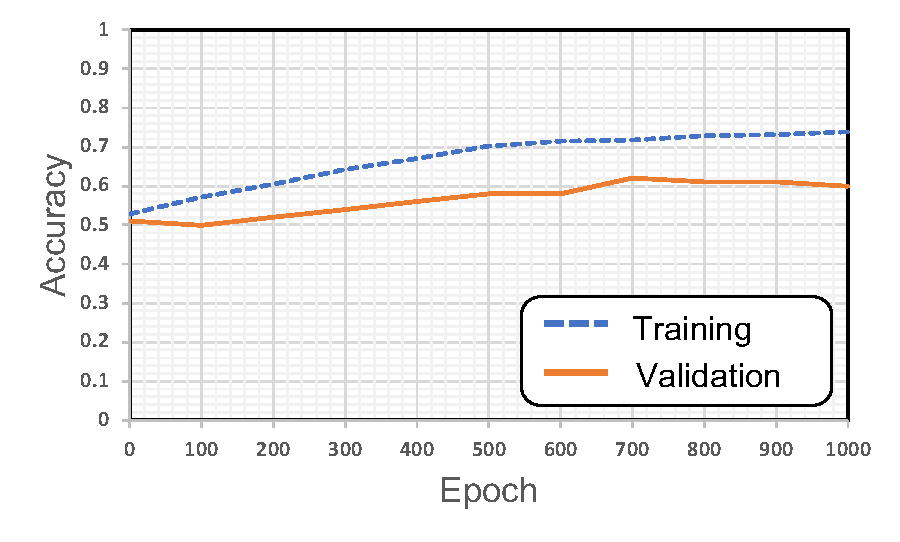
\includegraphics[clip, width=4.5in]{figures/graph/stripe_1block99ratio.pdf}
    \label{fig:acc_stripe_99ratio_1block}}
    \\
    \subfloat[Spectrogram of estimated signal and predictive separation signal.]{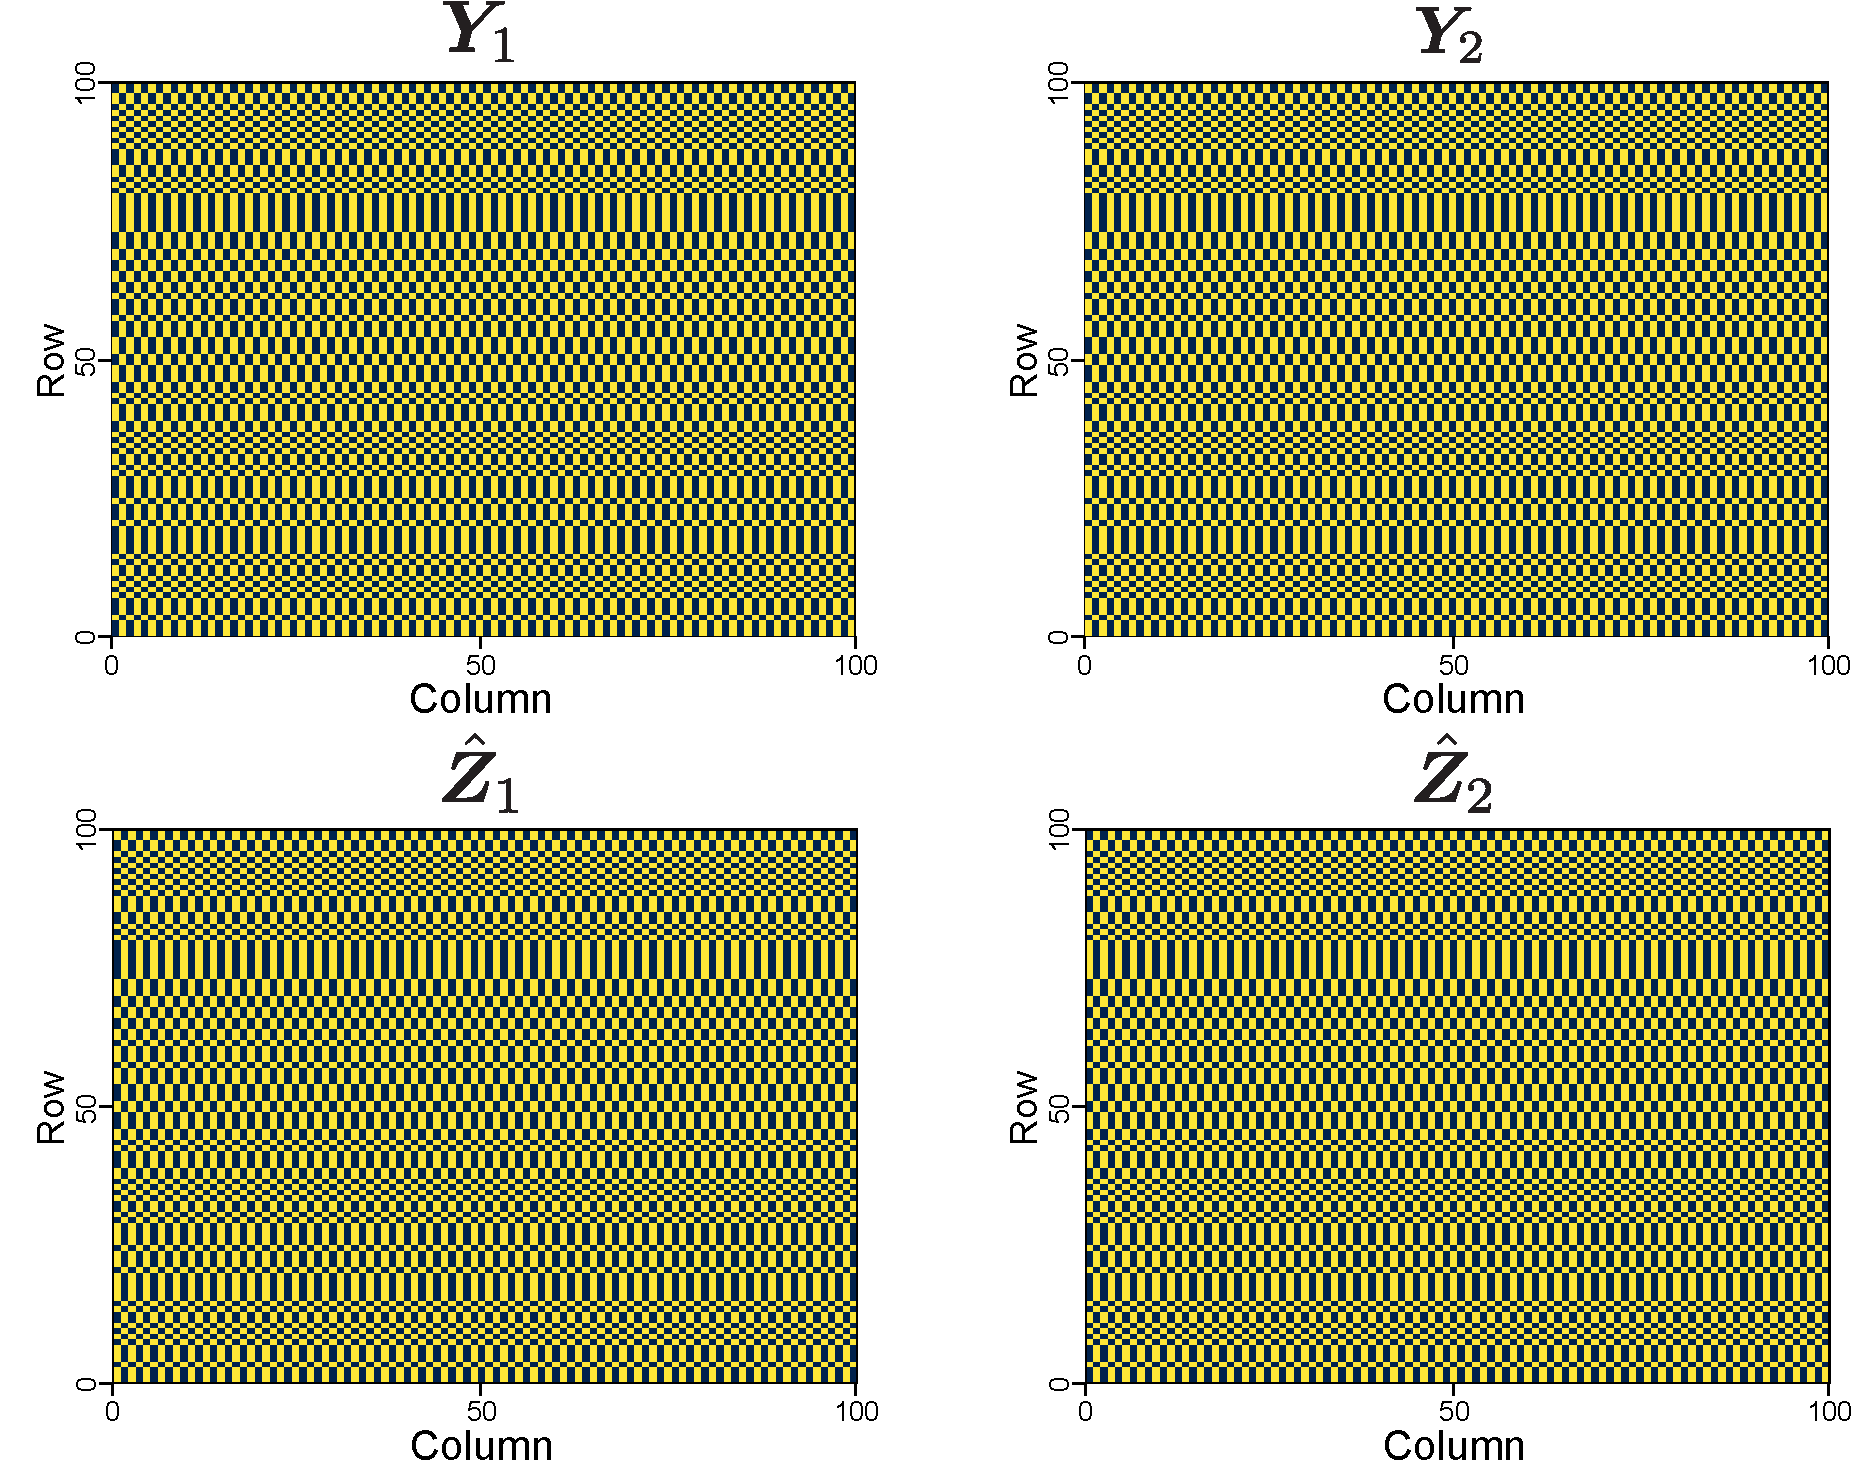
\includegraphics[clip, width=5.0in]{figures/stripe99ratio_1block_spec.pdf}
    \label{fig:spec_stripe_99ratio_1block}}  
    \caption{Experimental results using the matrix of Fig~\ref{fig:stripe_spec} (randomly shuffle per row, then 1\% chance to set two rows).}
    \label{fig:stripe_99ratio_1block}
\end{figure*}
%%%%%%%%%%%%%%%%%%%%%%%%%%%%

%%%%%%%%%%%%%%%%%%%%%%%%%%%%
\begin{figure*}[!t]
  \centering
  \subfloat[Percentage of correct answers for training and validation data.]{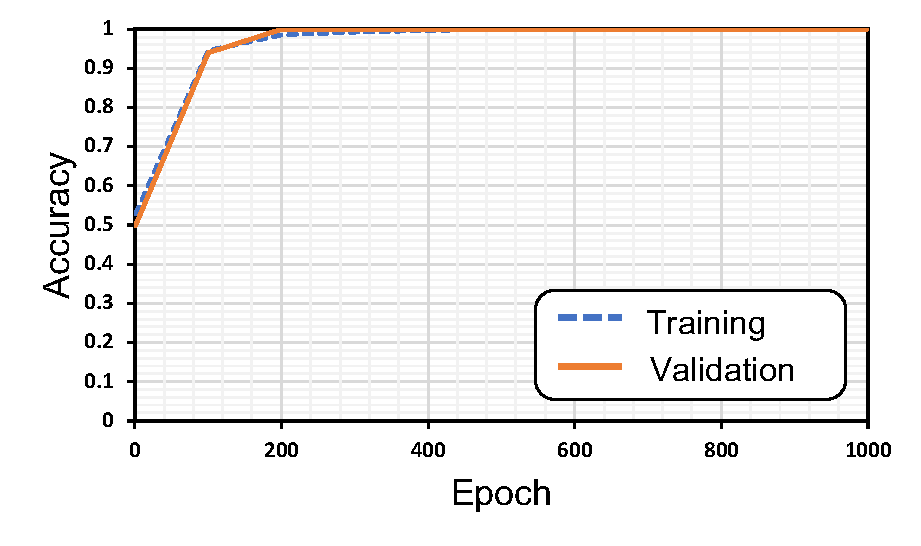
\includegraphics[clip, width=4.5in]{figures/graph/01mat_2block.pdf}
  \label{fig:acc_01mat_2block}}
  \\
  \subfloat[Spectrogram of estimated signal and predictive separation signal.]{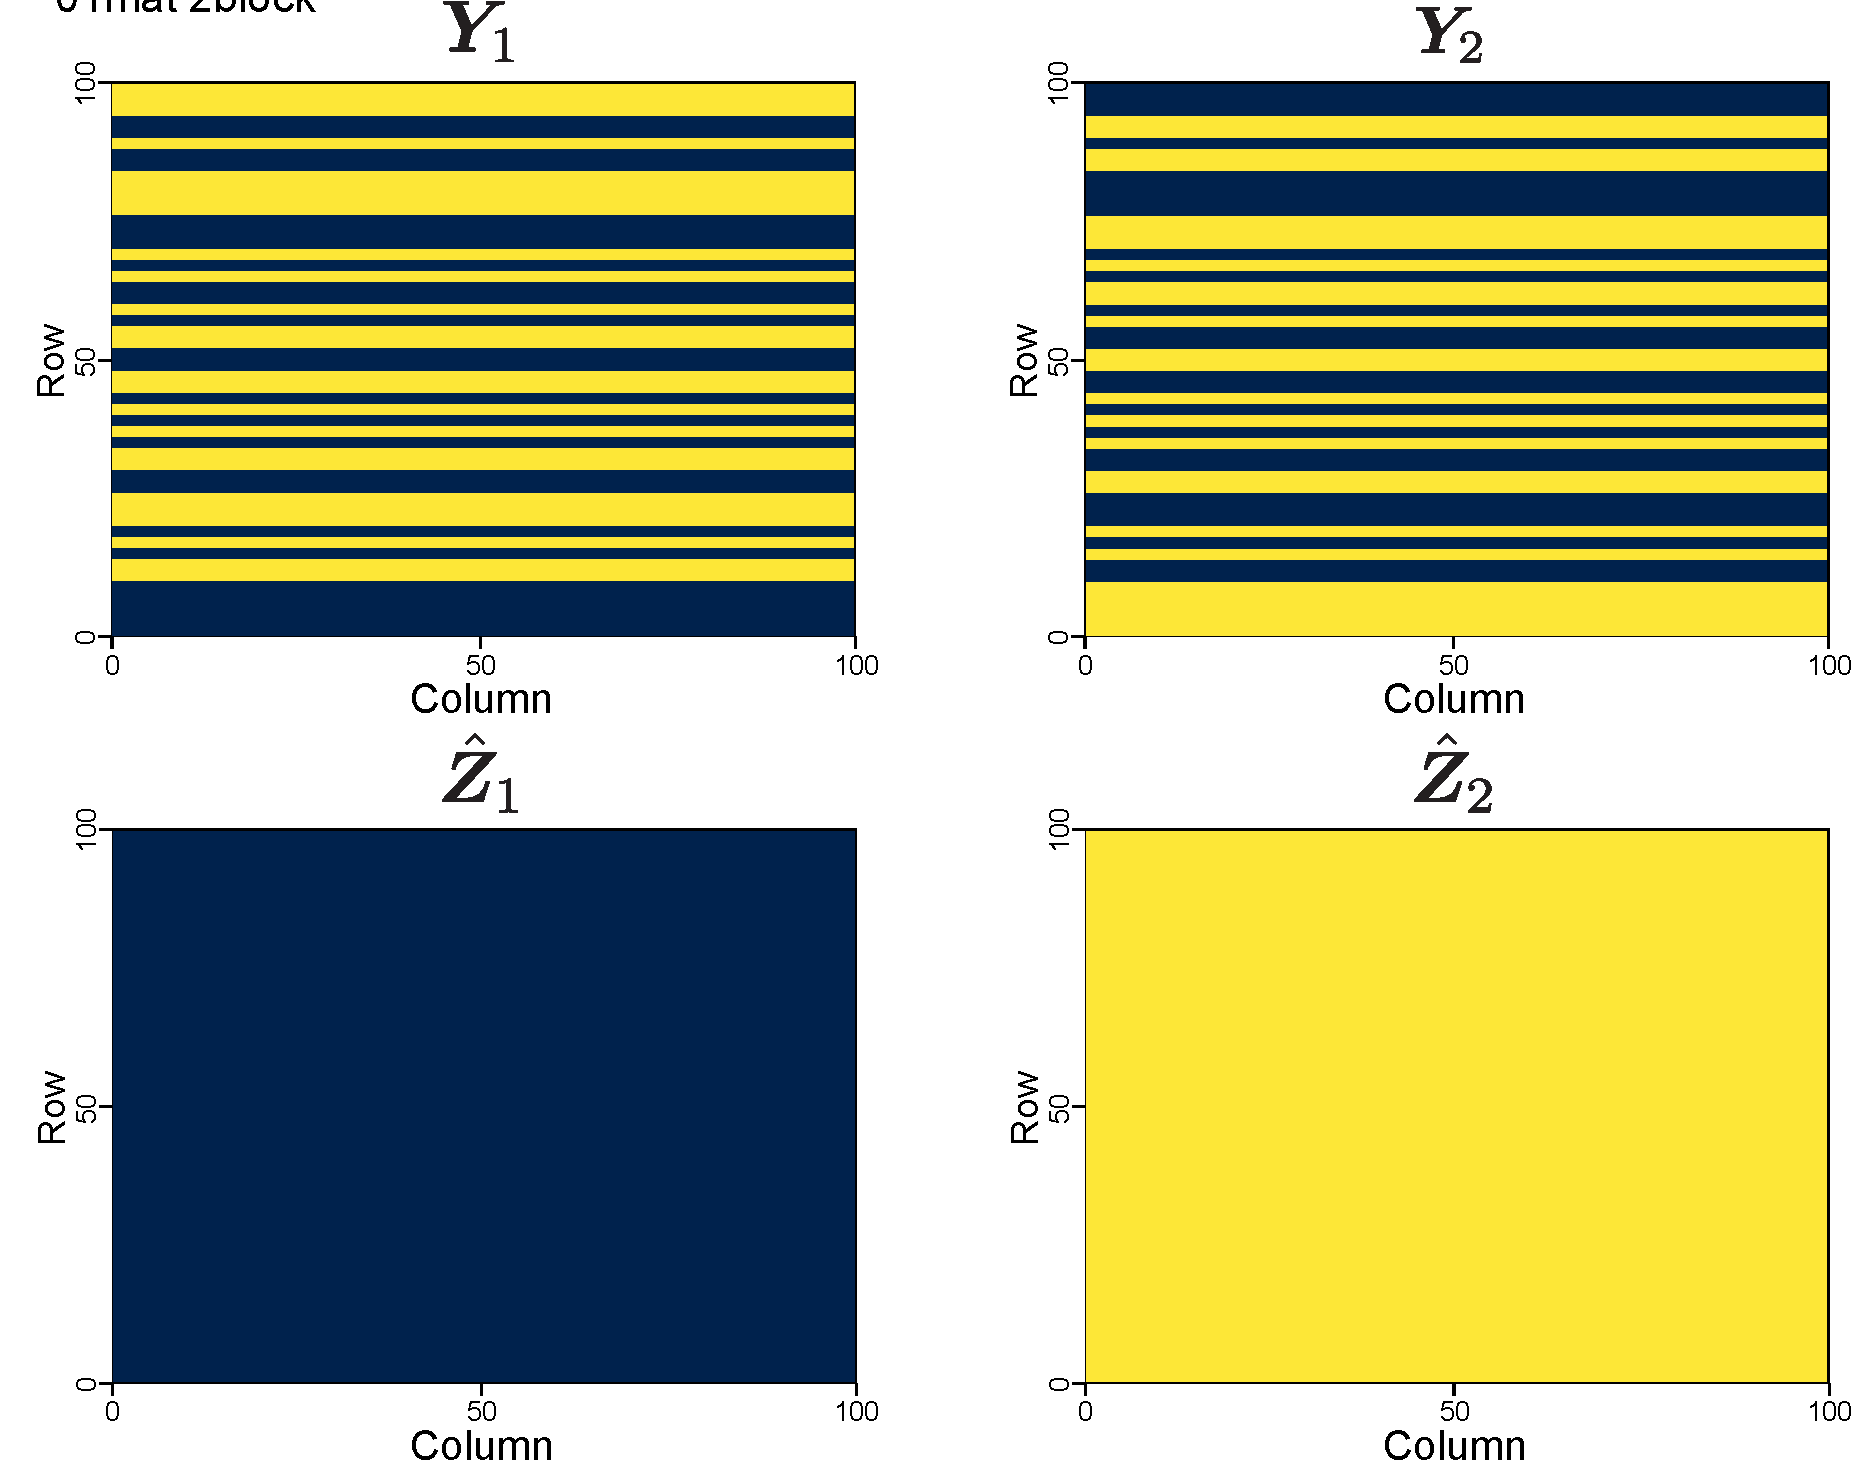
\includegraphics[clip, width=5.0in]{figures/01mat_2block.pdf}
  \label{fig:spec_01mat_2block}}
  \caption{Experimental results using the matrix of Fig~\ref{fig:01mat_spec} (randomly shuffle every two rows).}
  \label{fig:01mat_2block}
\end{figure*}
%%%%%%%%%%%%%%%%%%%%%%%%%%%%

%%%%%%%%%%%%%%%%%%%%%%%%%%%%
\begin{figure*}[!t]
  \centering
  \subfloat[Percentage of correct answers for training and validation data.]{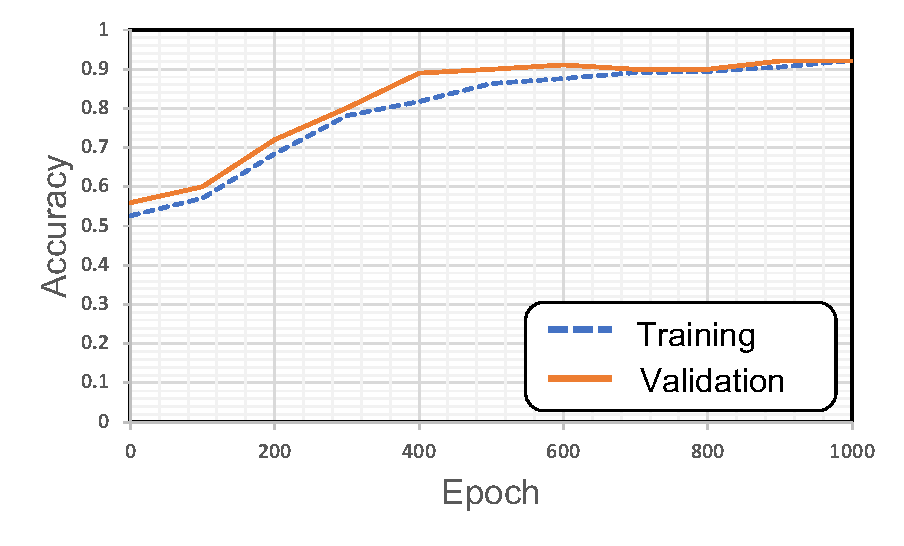
\includegraphics[clip, width=4.5in]{figures/graph/25stripe_2block.pdf}
  \label{fig:acc_25stripe_2block}}
  \\
  \subfloat[Spectrogram of estimated signal and predictive separation signal.]{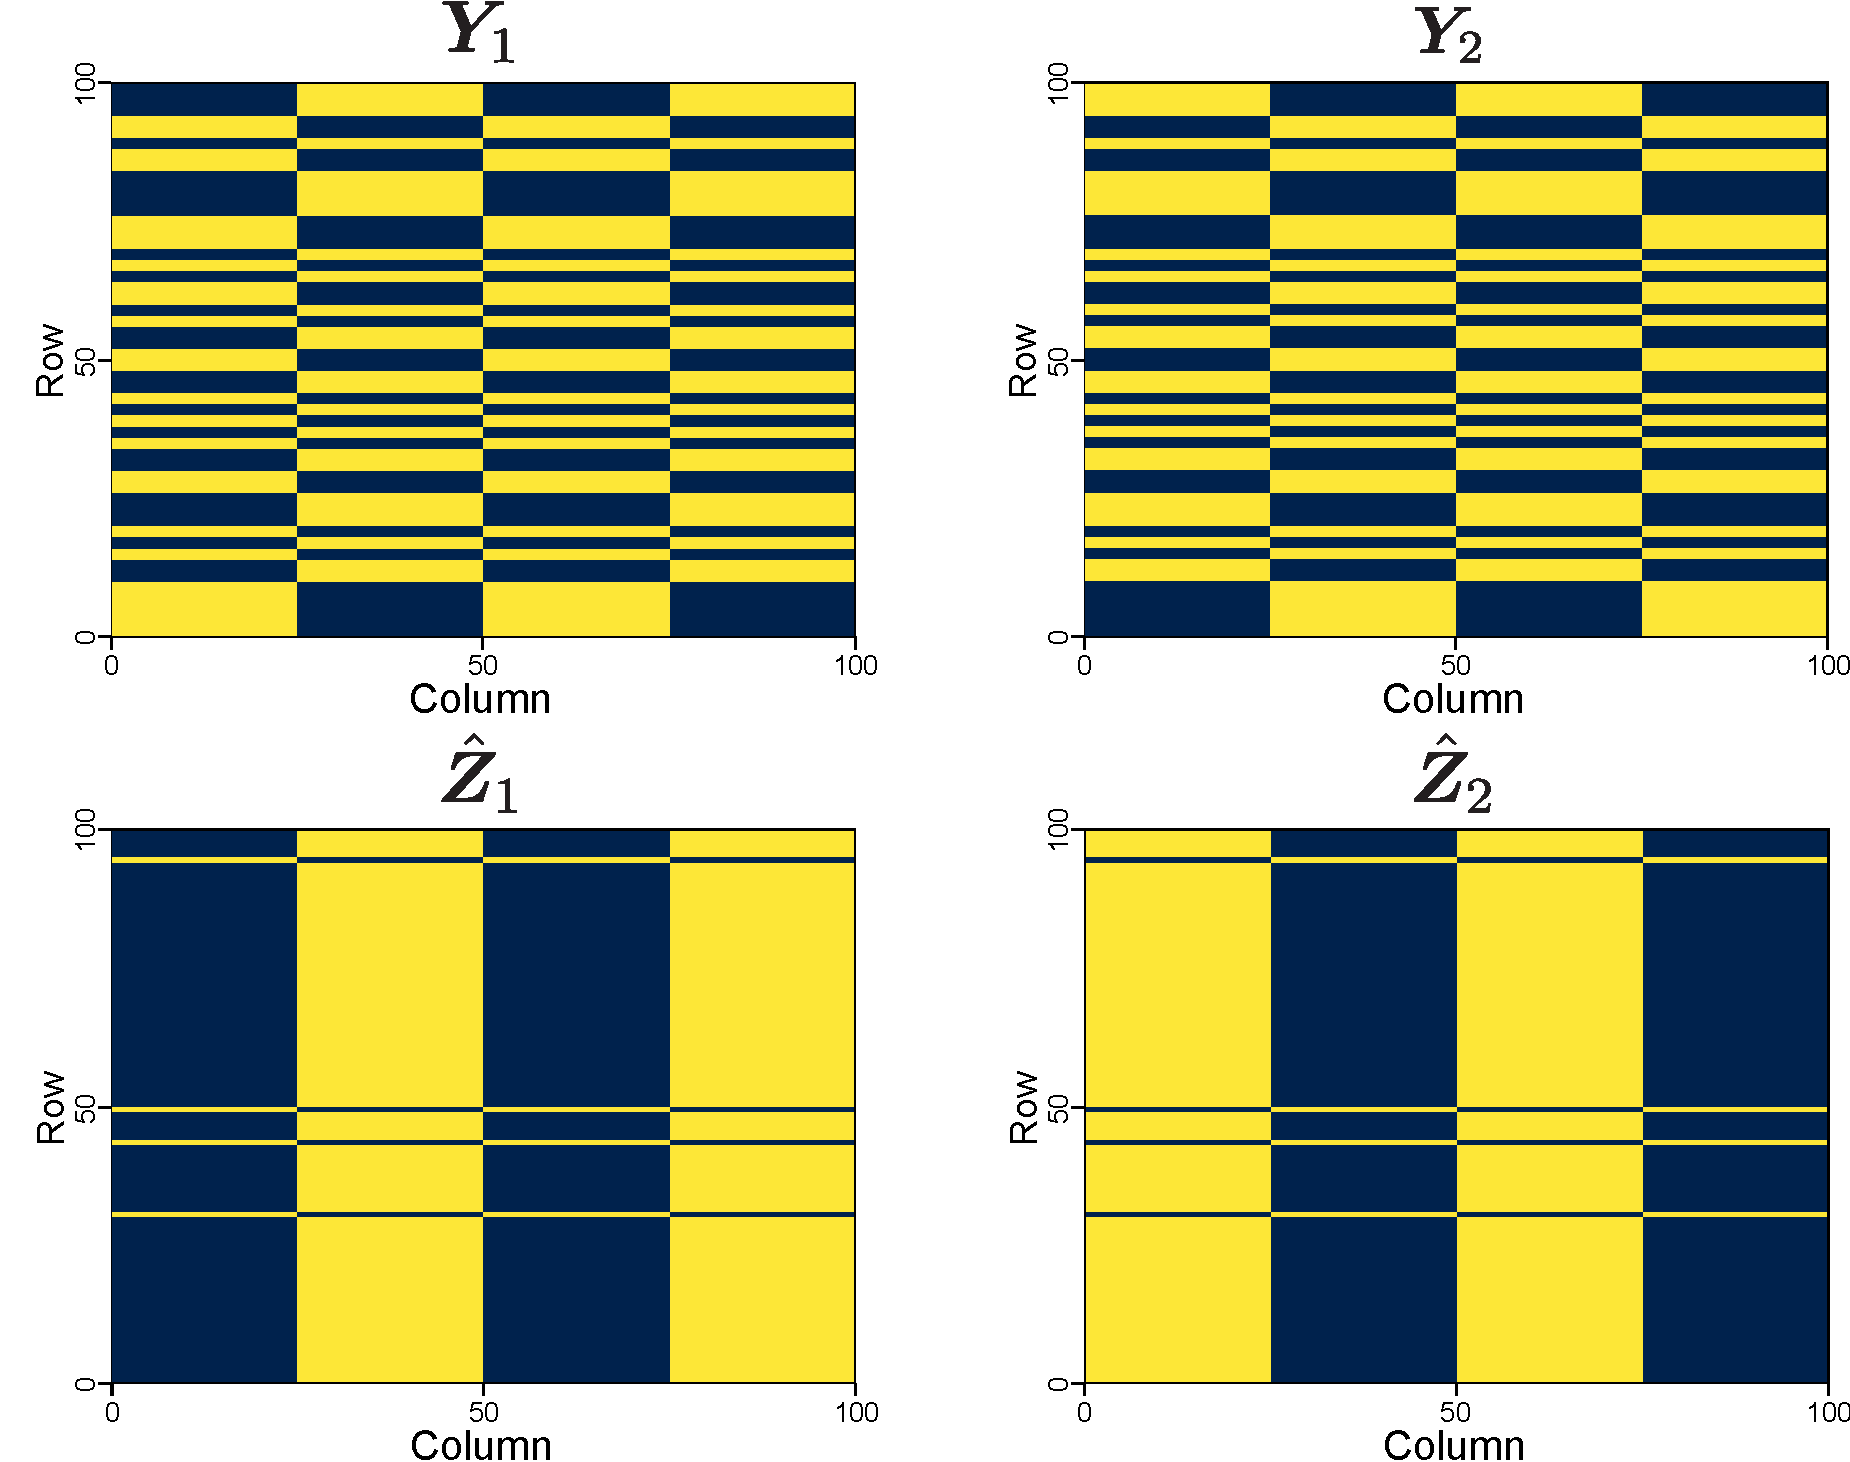
\includegraphics[clip, width=5.0in]{figures/25stripe_2block.pdf}
  \label{fig:spec_25stripe_2block}}
  \caption{Experimental results using the matrix of Fig~\ref{fig:25stripe_spec} (randomly shuffle every two rows).}
  \label{fig:25stripe_2block}
\end{figure*}
%%%%%%%%%%%%%%%%%%%%%%%%%%%%

%%%%%%%%%%%%%%%%%%%%%%%%%%%%
\begin{figure*}[!t]
  \centering
  \subfloat[Percentage of correct answers for training and validation data.]{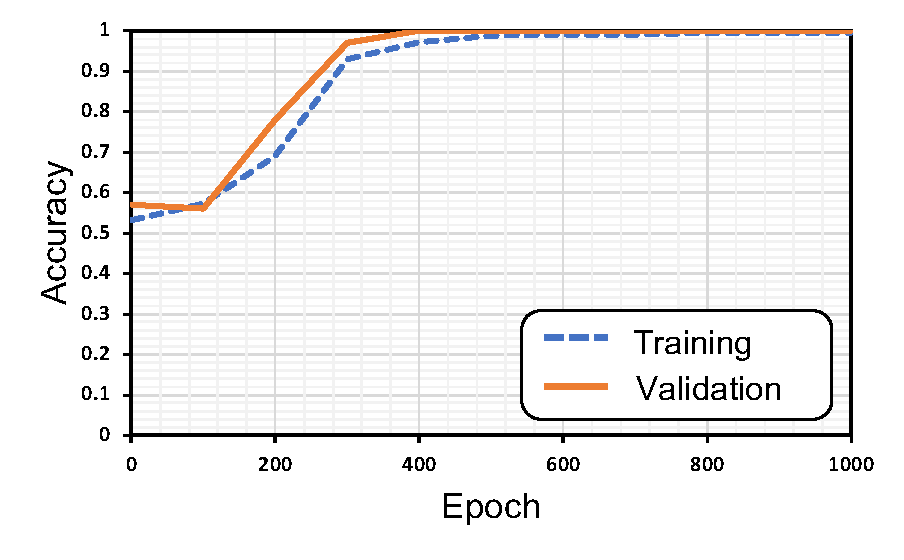
\includegraphics[clip, width=4.5in]{figures/graph/stripe_2block.pdf}
  \label{fig:acc_stripe_2block}}
  \\
  \subfloat[Spectrogram of estimated signal and predictive separation signal.]{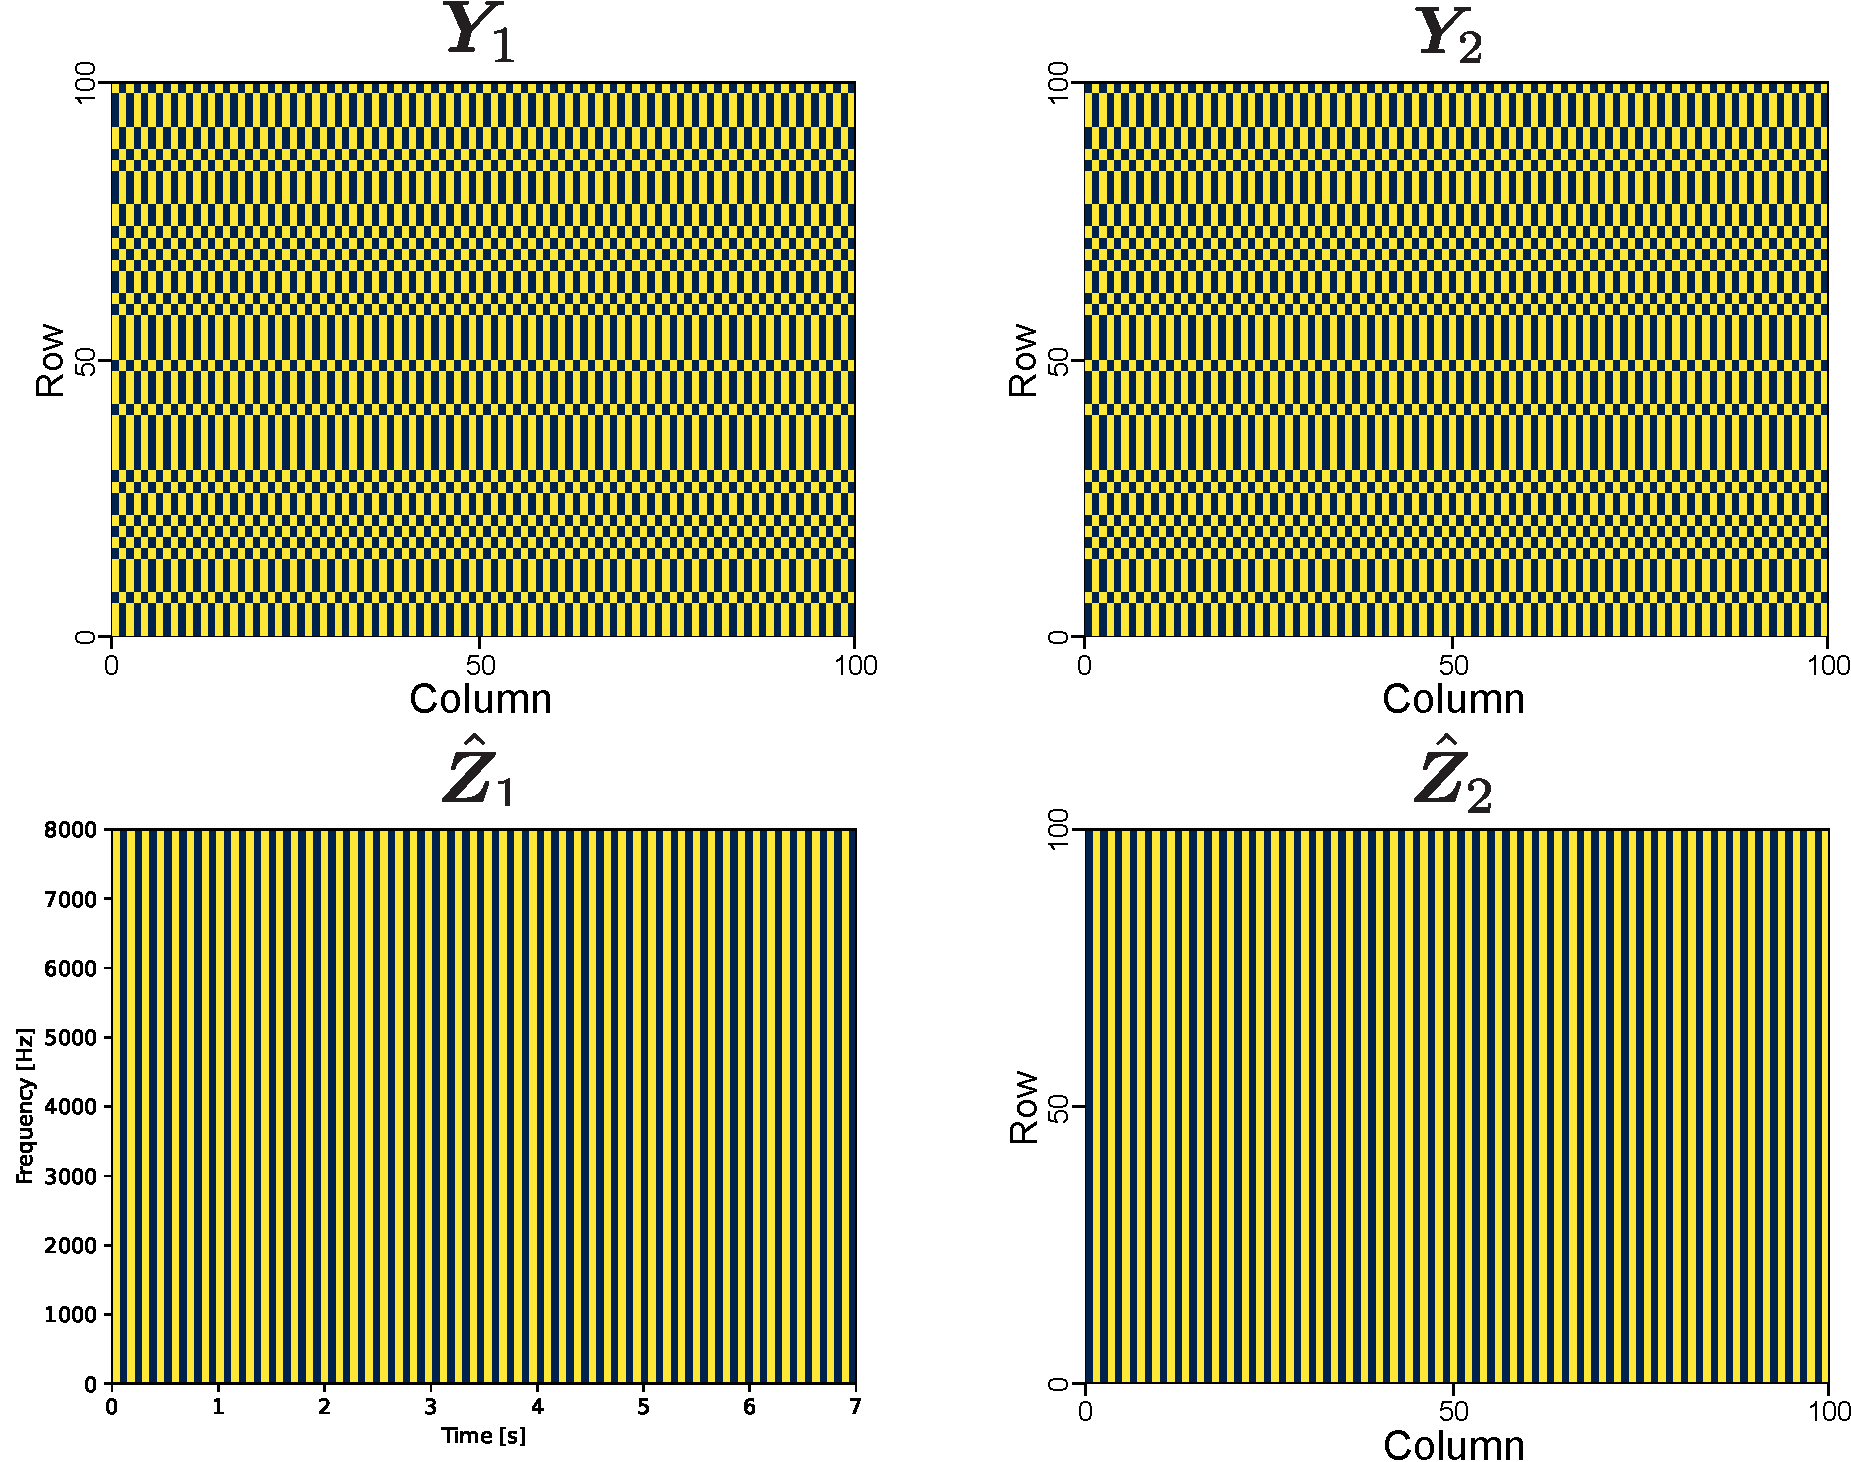
\includegraphics[clip, width=5.0in]{figures/stripe_2block.pdf}
  \label{fig:spec_stripe_2block}}
  \caption{Experimental results using the matrix of Fig~\ref{fig:stripe_spec} (randomly shuffle every two rows).}
  \label{fig:stripe_2block}
\end{figure*}
%%%%%%%%%%%%%%%%%%%%%%%%%%%%


\clearpage
%----------------------------------------------
\subsection{音声及び音楽信号に対する実験結果}
\label{sec:ex_res_artificial}
%----------------------------------------------

%%%%%%%%%%%%%%%%%%%%%%%%%%%%
\begin{figure*}[!t]
  \centering
  \subfloat[Percentage of correct answers for training and validation data.]{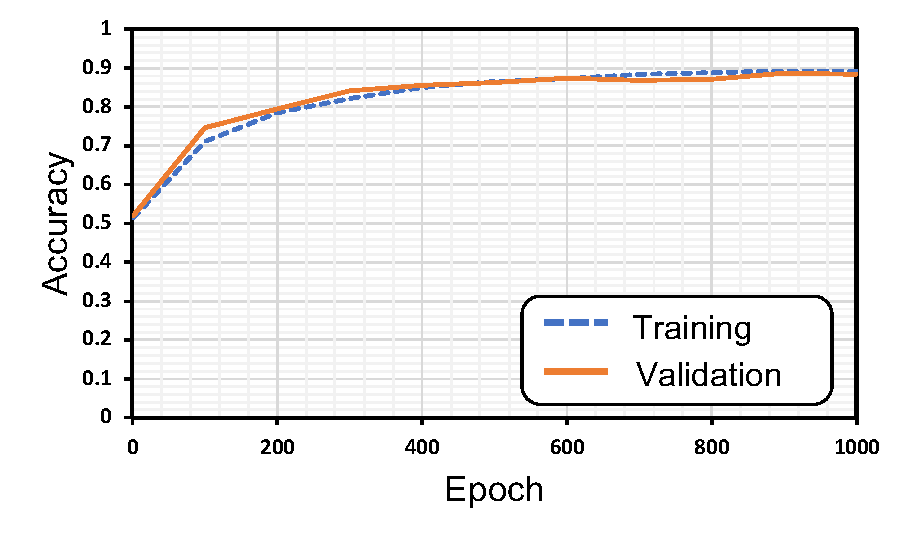
\includegraphics[clip, width=4.5in]{figures/graph/audio_16block.pdf}
  \label{fig:acc_audio_16block}}
  \\
  \subfloat[Spectrogram of estimated signal and predictive separation signal.]{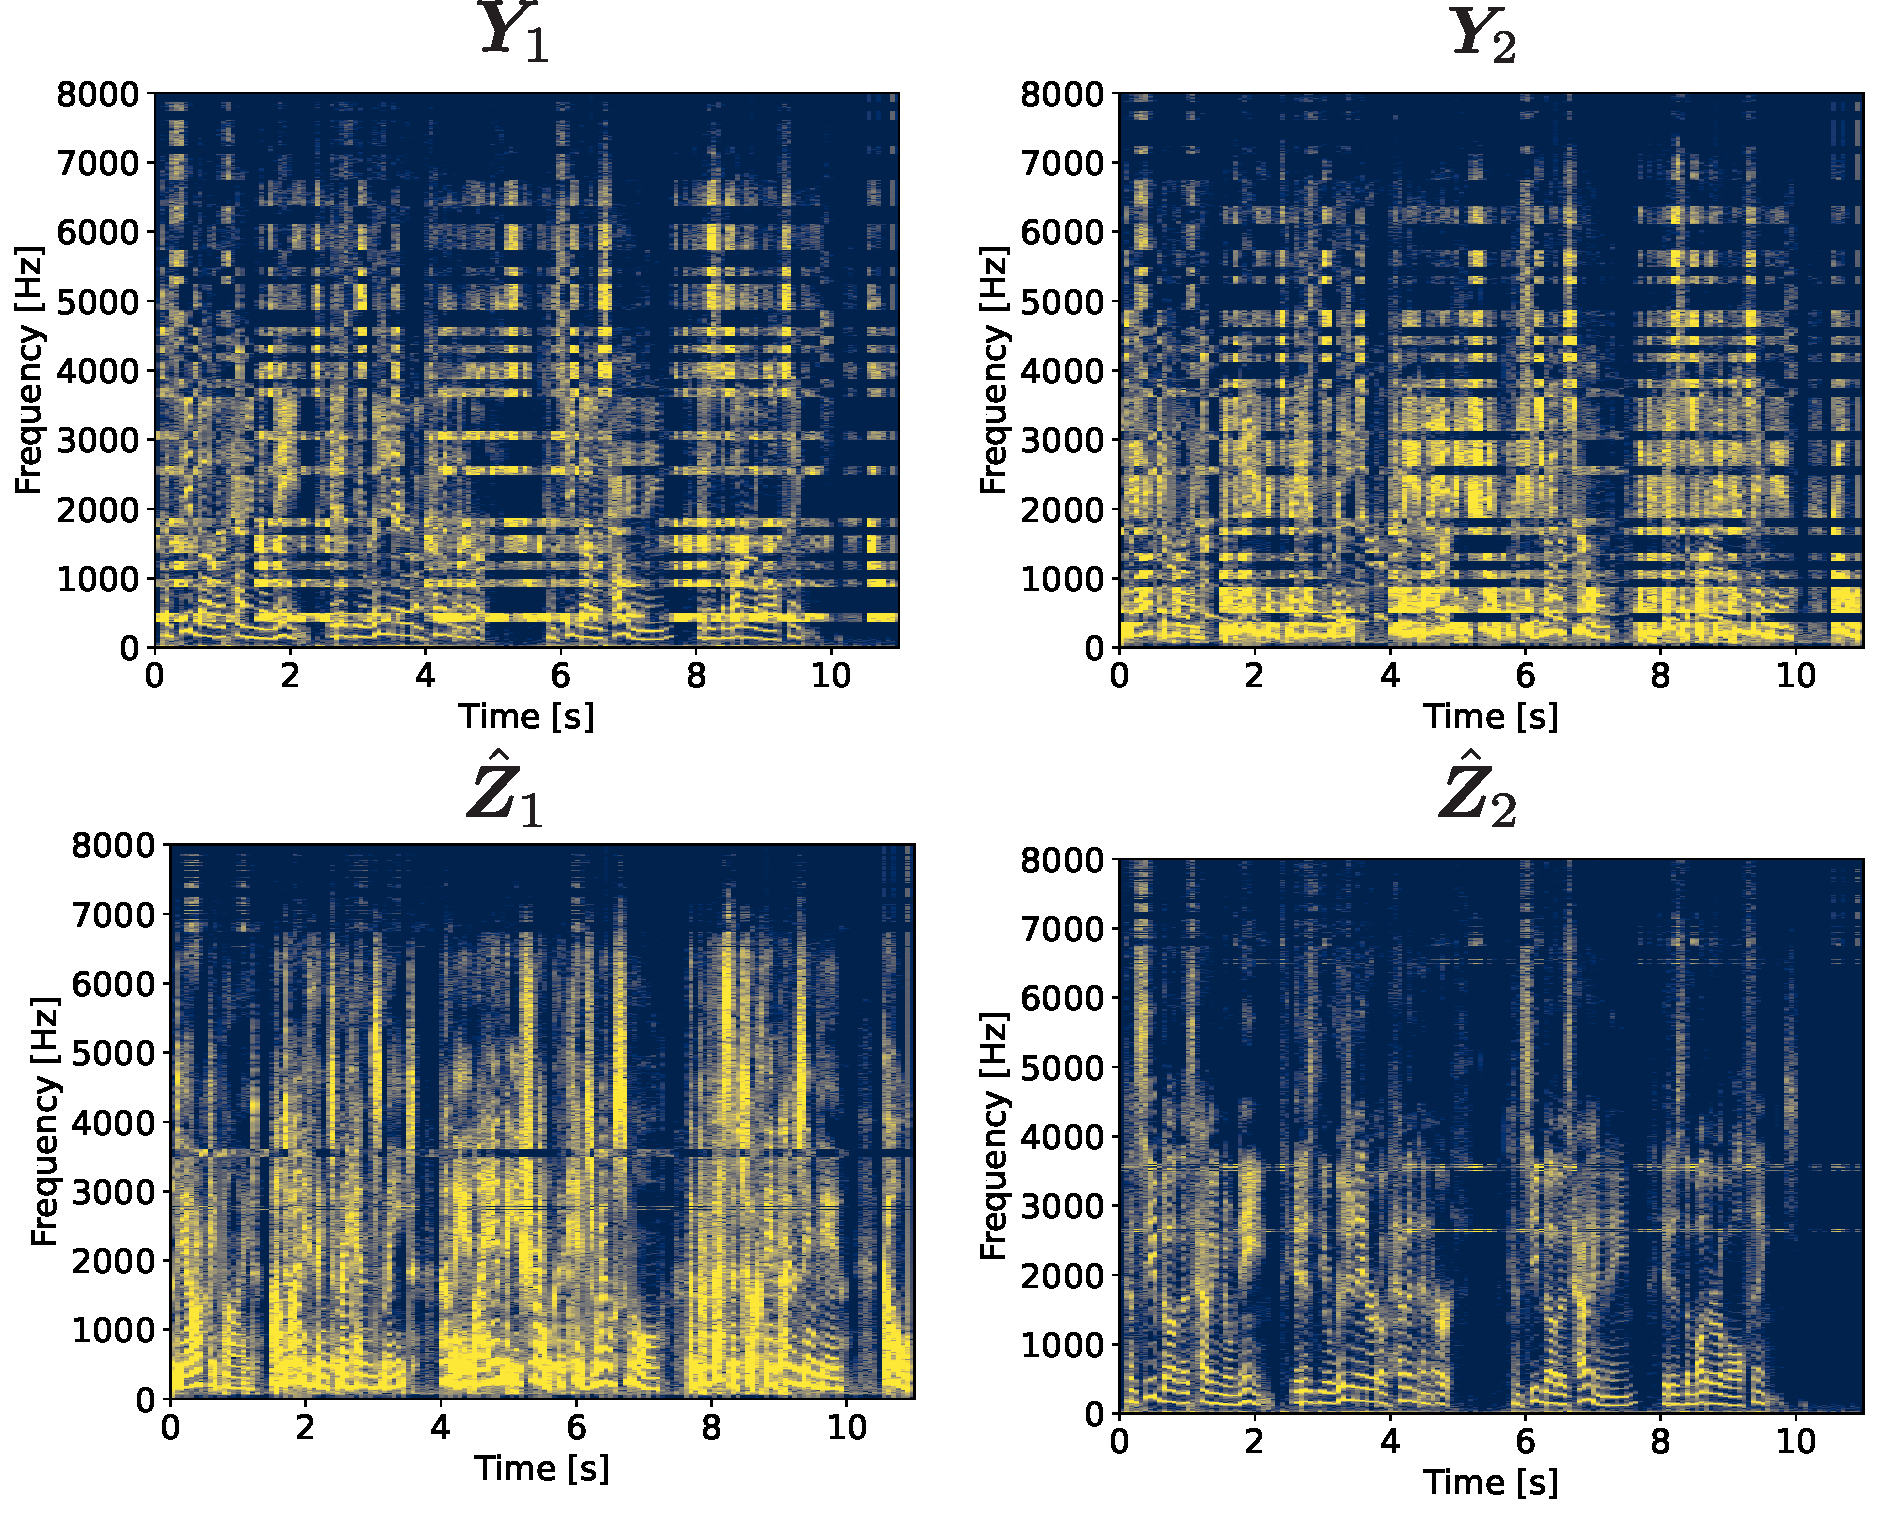
\includegraphics[clip, width=5.0in]{figures/audio_16block.pdf}
  \label{fig:spec_audio_16block}}
  \caption{Experimental results using audio signal of Fig~\ref{fig:audio} (shuffle the frequency every sixteen rows).}
  \label{fig:audio_16block}
\end{figure*}
%%%%%%%%%%%%%%%%%%%%%%%%%%%%

%%%%%%%%%%%%%%%%%%%%%%%%%%%%
\begin{figure*}[!t]
  \centering
  \subfloat[Percentage of correct answers for training and validation data.]{\includegraphics[clip, width=4.5in]{figures/graph/Drum_16block.pdf}
  \label{fig:acc_Drum_16block}}
  \\
  \subfloat[Spectrogram of estimated signal and predictive separation signal.]{\includegraphics[clip, width=5.0in]{figures/Drum_16block.pdf}
  \label{fig:spec_Drum_16block}}  
  \caption{Experimental results using instrumental sound of Fig~\ref{fig:drum} (shuffle the frequency every sixteen rows).}
  \label{fig:Drum_16block}
\end{figure*}
%%%%%%%%%%%%%%%%%%%%%%%%%%%%

Fig.~\ref{fig:audio_16block}は音声信号を用いた時の結果であり,Fig.~\ref{fig:Drum_16block}は楽器音を用いた時の結果である.
音声信号,楽器音のどちらに対しても,検証データの正答率が90\%を超えており,$\hat{\bm{Z}}_1$,$\hat{\bm{Z}}_2$を概ね的確に推定できていることが分かる.
SDRの改善量は,Fig.~\ref{fig:audio_16block}の$\hat{\bm{Z}}_1$に対して25~dB,$\hat{\bm{Z}}_2$に対して31~dBであった.
また,Fig.~\ref{fig:Drum_16block}の$\hat{\bm{Z}}_1$に対して17~dB,$\hat{\bm{Z}}_2$に対して18~dBであった.
Fig.~\ref{fig:audio_16block}とFig.~\ref{fig:Drum_16block}を比較すると,楽器音を用いた実験の方が,音声信号を用いた実験よりも検証データに対する正答率が高いことが分かる.
これは,使用した楽器音(ドラムとピアノ)は,音声信号に比べてそれぞれの音の違いが明確であるからだと推測できる.
ドラムの音は,Fig.~\ref{fig:drum}の$\bm{Z}_1$のスペクトログラムに示すように,全周波数成分に対して値を保持している.
一方で,ピアノの音はFig.~\ref{fig:drum}の$\bm{Z}_2$のスペクトログラムに示すように,周波数成分に対して一定の間隔を保ちながら,値を保持していることが分かる.
これらの楽器音の違いにより,DNNは音声信号より楽器音の方が高精度で推定分離信号を予測することができたと考えられる.
今回の実験より,ある程度の塊毎に各周波数成分のシャッフルが行われているときは,実際の音声信号や楽器音でもDNNは高精度で分離信号を予測することが可能だと分かる.

\clearpage
%----------------------------------------------
\section{本章のまとめ}
\label{sec:matome}
%----------------------------------------------
本章では,提案手法の有効性を確認するため,人工的に作成したデータと実際の音声及7音楽信号を用意し実験を行った.
実験の結果より,人工データを用いたブロック単位でのパーミュテーション問題に対しては,どのような行列であっても100\%に近い確率で解決できることを示した.
実際の音声データに対しても,ブロック単位でシャッフルが行われていると90\%を超える正答率になることを示した.
SDRの改善量は,音声データに対して25~dB程度,楽器音に対しては17~dB程度であった.
次章では,本論文における総括とした結論を述べる.


%%%%% 第5章 %%%%%
\chapter{結言}
\label{chap:con}

本論文では,FDICAに伴うパーミュテーション問題の解決を目的とし,深層パーミュテーション解決法を新たに提案した.
DNNの入力には,正規化した分離信号から局所時間振幅スペクトログラム成分を抽出した値を用いた.
DNNの出力には,softmax関数を使用し確率値を出力する.この確率値は,各音源の成分である確率を意味する.
DNNの出力である確率値を用いて,推定パーミュテーション行列を作成し分離信号の並び替えを行った.
損失関数にはMSEを用い,推定分離信号と完全分離信号のスペクトログラム間で損失を求め誤差逆伝搬を行った.
テストデータに対してはDNNの入力となる局所時間振幅スペクトログラムをストライド幅に従ってずらしていくことで,時間方向に対して多数決処理を行った.
実験結果より,ブロック単位でのパーミュテーション問題に対しては提案手法を用いて正しく並び替えができることを示した.

最後に今後の展望を述べる.
本論文では,深層パーミュテーション解決手法の可能性に注目しており,基礎的な実験を行ってきた.
本実験では,学習データと検証データの音源に同じスペクトログラムを用いて実験を行っており,未だに音源の時間周波数構造に対する汎化性能は獲得できていない.
この問題を解決するためには,学習データに多数の音声及び音楽信号を用意し,大量のデータをDNNに学習させる必要がある.
また,更なる精度向上のために,DNNの構造としてMLPを用いるのではなく,双方向再帰型DNNを使用することを検討している.
さらには,2音源の実験の拡張版として3音源以上に対する実験も行う必要がある.


%%%%%%%%%%%%%%%%%%%%%%%%%%% 後付 %%%%%%%%%%%%%%%%%%%%%%%%%%%
\backmatter

%%%%% 謝辞 %%%%%
\chapter{謝辞}

本論文は,香川高等専門学校電気情報工学科北村研究室にて行われた研究に基づくものです.

まず,本研究を進めるにあたり,ご多忙のところ熱心に
ご指導くださいました指導教員の北村大地講師に心より感謝申し上げます.
北村大地講師には,論文執筆や研究に関する議論など,細部にわたるまで
丁寧にご指導いただきました.DNNの研究で用いるサーバの増設等にも取り組んでいただき,日々の研究を効率良く行うことができました.心よりありがたくお礼申し上げます.
本論の副査である雛元洋一助教には,論文の構成や記述に関して有益な助言を頂き,大変お世話になりました.ここに厚く御礼申し上げます.
北村研究室の先輩である専攻科2年の岩瀬佑太氏,大藪宗一郎氏,梶谷奈未氏,渡辺瑠伊氏には,音源分離に関する基礎概念のご説明をはじめ,研究の進め方に関して数々のご支援をいただきました.
特に,北村研究室の先輩である専攻科2年の渡辺瑠伊氏には,DNNに関するアドバイスやサーバ管理に関する知見をはじめ,数々のご支援とご助言をいただきました.心より感謝申し上げます.
また,北村研究室同期の川口翔也氏,細谷泰稚氏,村田佳斗氏,溝渕悠朔氏には,日頃のディスカッションのほか,1年に亘る研究室生活を様々な面で支えていただきました.
ここに感謝申し上げます.

最後になりますが,現在に至るまで私の学生生活を金銭的に支え,
暖かく見守って下さった両親には感謝の念に堪えません.
これまで本当にありがとうございました.


%%%%% 参考文献(直接書く場合) %%%%%
\addcontentsline{toc}{chapter}{\bibname}
\begin{thebibliography}{99}
  % 参考文献が10以上ある場合は{99}とする
  %\itemsep -3pt             % 項目の間隔微調整用
  %\fontsize{7.5pt}{10pt}\selectfont
  
  \bibitem{BSS}
  H.~Sawada, N.~Ono, H.~Kameoka, D.~Kitamura, and H.~Saruwatari, ``A review of blind source separation methods: Two converging routes to ILRMA originating from ICA and NMF,'' \textit {APSIPA Trans. Signal and Information Processing}, vol. 8, no. e12, pp. 1--14, 2019.
  
  \bibitem{ICA}
  P.~Comon, ``Independent component analysis, a new concept?,'' \textit{Signal Processing}, vol. 36, no. 3, pp. 287--314, 1994.
  
  \bibitem{FDICA}
  P.~Smaragdis, ``Blind separation of convolved mixtures in the frequency domain,'' \textit{Neurocomputing}, vol. 22, pp. 21--34, 1998.
  
  \bibitem{COR}
  N.~Murata, S.~Ikeda, and A.~Ziehe, ``An approach to blind source separation based on temporal structure of speech signals,''  \textit{Neurocomputing}, vol. 41, no. 1--4, pp. 1--24, 2001.
  
  \bibitem{Permutation_solverBSS}
  H. Sawada, S. Araki, and S. Makino, ``Measuring dependence of bin-wise separated signals for permutation alignment in frequency-domain BSS,'' \textit{Proc. IEEE International Symposium on Circuits and Systems}, pp. 3247--3250, 2007.
  
  \bibitem{DOA}
  H.~Saruwatari, T.~Kawamura, T.~Nishikawa, A.~Lee, and K.~Shikano, ``Blind source separation based on a fast-convergence algorithm combining ICA and beamforming,''  \textit{IEEE Trans. Audio, Speech, and Language Processing}, vol. 14, no. 2, pp. 666--678, 2006.
  
  \bibitem{DOACOR}
  H.~Sawada, R.~Mukai, S.~Araki, and S.~Makino, ``A robust and precise method for solving the permutation problem of frequency-domain blind source separation,''  \textit{IEEE Trans. Speech and Audio Processing}, vol. 12, no. 5, pp. 530--538, Sep. 2004.
  
  \bibitem{IVA1}
  T.~Kim, H.~T.~Attias, S.-Y.~Lee, and T.-W.~Lee, ``Blind source separation exploiting higher-order frequency dependencies,'' \textit{IEEE Trans. Audio, Speech, and Language Processing}, vol. 15, no. 1, pp. 70--79, 2007.
  
  \bibitem{IVA2}
  N.~Ono, ``Stable and fast update rules for independent vector analysis based on auxiliary function technique,'' \textit{Proc. IEEE Workshop on Applications of Signal Processing to Audio and Acoustics}, pp. 189--192, 2011.
  
  \bibitem{NMF}
  D.~D.~Lee and H.~S.~Seung, ``Learning the parts of objects by non-negative matrix factorization,'' \textit{Nature}, vol. 401, pp. 788--791, 1999.
  
  \bibitem{ILRMA1}
  D.~Kitamura, N.~Ono, H.~Sawada, H.~Kameoka, and H.~Saruwatari, ``Determined blind source separation unifying independent vector analysis and nonnegative matrix factorization,''  \textit{IEEE/ACM Trans. Audio, Speech, and Language Processing}, vol. 24, no. 9, pp. 1626--1641, 2016.
  
  \bibitem{ILRMA2}
  D.~Kitamura, N.~Ono, H.~Sawada, H.~Kameoka, and H.~Saruwatari, ``Determined blind source separation with independent low-rank matrix analysis,'' in  \textit{Audio Source Separation}, S. Makino, Ed., pp. 125--155. Springer, Cham, 2018.
  
  \bibitem{EU}
  D.~Kitamura, N.~Ono, and H.~Saruwatari, ``Experimental analysis of optimal window length for independent low-rank matrix analysis,''  \textit{Proc. European Signal Processing Conference}, pp.~1210--1214, 2017.

  \bibitem{DNN_soluver}
  S.~Yamaji and D.~Kitamura, ``DNN-based permutation solver for frequency-domain independent component analysis in two-source mixture case,'' \textit{Proc. APSIPA Annual Summit and Conference}, pp. 781--787, 2020.
  
  %\bibitem{preASJ}
  %  山地修平, 北村大地,
  %  ``局所時間周波数構造に基づく深層パーミュテーション解決法,''
  %  \textit{日本音響学会2020年春季研究発表会講演論文集}, pp.~317--320, 2020.
  
  \bibitem{Matsuoka2001_PB}
  K.~Matsuoka and S.~Nakashima, ``Minimal distortion principle for blind source separation,'' \textit{Proc. International Conference on Independent Component Analysis and Blind Signal Separation}, pp. 722--727, 2001.
  
  \bibitem{brock_p}
  Y.~Liang, S.M.~Naqvi, and J.~Chambers, ``Overcoming block permutation
  problem in frequency domain blind source separation when using
  AuxIVA algorithm,'' \textit{Electron. Lett}, pp.460--462, 2012.

  \bibitem{User_anotation}
  \red{F. Oshima, M. Nakano, and D. Kitamura, ``Interactive speech source separation based on independent low-rank matrix analysis,'' \textit{Acoustical Science and Technology}, vol. 42, no. 4, pp. 222--225, 2021.}
  %Y.~Mitsui, D.~Kitamura, N.~Takamune, H.~Saruwatari,
  %Y.~Takahashi, and K.~Kondo, ``Independent low-rank matrix analysis based on %parametric majorizaion-equalization
  %algorithm,'' \textit{Proc. CAMSAP}, pp.98–102, 2007.
  
  \bibitem{stiching}
  \red{T. Neumann, K. Kinoshita, C. Boeddeker, M. Delcroix, and R. Umbach, ``Graph-PIT: Generalized permutation invariant training for continuous separation of arbitrary numbers of speakers,'' \textit{INTERSPEECH}, pp. 3490--3494, 2021.}

  \bibitem{PIT}
  \red{ D. Yu, M. Kolbak, Z.-H. Tan, and J. Jensen, ``Permutation invariant training of deep models for speaker-independent multi-talker speech separation,'' \textit{Proc. IEEE International Conference on Acoustics, Speech and Signal Processing}, pp. 241-245, 2017. }

  \bibitem{BSSEval}
  E.~Vincent, R.~Gribonval, and C.~F\'{e}votte, ``Performance measurement in blind audio source separation," \textit{IEEE Trans. Audio, Speech, and Language Processing}, vol.~14, no.~4, pp.~1462--1469, 2006.
  
  \bibitem{relu}
  V.~Nair and G.~E.~Hinton, ``Rectified linear units improve restricted boltzmann machines,'' 
  \textit{Proc. International Conference on Machine Learning}, 2010.
  
  \bibitem{Sisec}
  S.~Araki, F.~Nesta, E.~Vincent, Z.~Koldovsky, G.~Nolte, A.~Ziehe, and A.~Benichoux, ``The 2011 signal separation evaluation campaign (SiSEC2011): -Audio source separation,'' \textit{Proc. International Conference on Latent Variable Analysis and Signal Separation}, pp. 414--422, 2012.
  
  \bibitem{adam}
  D.~P.~Kingma and J.~Ba, ``Adam: A method for stochastic optimization,''
  \textit{arXiv preprint arXiv}, pp. 1412--6980, 2014.
  %\bibitem{DuongMethod}
  %N.~Q.~K.~Duong, E.~Vincent, and R.~Gribonval, ``Under-determined reverberant audio %source separation using a full-rank spatial covariance model," \textit{IEEE Trans. %ASLP}, vol.~18, no.~7, pp.~1830--1840, 2010.
  
\end{thebibliography}


%%%%% 参考文献(BibTeXを使う場合) %%%%%
% \addcontentsline{toc}{chapter}{\bibname} % 参考文献を目次に表示
% \bibliography{ref_abb_full,references}

%%%%% 発表文献一覧 %%%%%
% {
% \chapter*{発表文献一覧}
% \newcommand{\myname}[1]{\textbf{\underline{#1}}}

% \section*{査読付き国際会議}
% \begin{enumerate}
%   \item \myname{Taro~Kosen} and Daichi~Kitamura,
%     ``Awesome method for surprising something,'' 
%     in Proceedings of \emph{{IEEE} International Conference on Something Awesome}, 
%     2018, pp. 100--103.
%   \item \myname{Taro~Kosen}, Hanako~Kagawa, and Daichi~Kitamura,
%     ``Very awesome method for surprising something,'' 
%     in Proceedings of \emph{{IEEE} International Conference on Something Awesome}, 
%     2019, pp. 100--103.
% \end{enumerate}


% \section*{国内学会}
% \begin{enumerate}
%   \item  \myname{高専太郎}, 北村大地, 
%     ``驚くべき何かの為の素晴らしい手法,''
%     日本何らか学会 2018年春季研究発表会講演論文集, 1-1-10, pp. 100--101, 2018.
%   \item  \myname{高専太郎}, 香川花子, 北村大地, 
%     ``さらに驚くべき何かの為の素晴らしい手法,''
%     日本何らか学会 2019年春季研究発表会講演論文集, 1-1-10, pp. 100--101, 2019.
% \end{enumerate}


% \section*{受賞}
% \begin{enumerate}
%   \item 日本何らか学会 第10回 優秀学生発表賞
% \end{enumerate}
% }


%%%%%%%%%%%%%%%%%%%%%%%%%%% 付録 %%%%%%%%%%%%%%%%%%%%%%%%%%%
\appendix

%%%%% 付録A %%%%%
% \chapter{DNNの人工データに対する予測結果}
% \label{chap:artificial}

% %----------------------------------------------
% \section{接線不等式}
% %----------------------------------------------

% \begin{lemm} \label{lem:aux:sessen} (接線不等式)
% $f(x)$が凹関数であるとき,以下の不等式が成立する.
% \begin{align}
% f(x) \leq f'(\bar{x}) (x - \bar{x}) + f(\bar{x})
% \end{align}
% 不等式中の等号が成立するための条件は$x = \bar{x}$である.
% \end{lemm}

% %----------------------------------------------
% \section{Jensenの不等式}
% %----------------------------------------------

% \begin{lemm} \label{lem:aux:jensen} (Jensenの不等式)
% $\alpha_{i} > 0$を,$\sum_{i} \alpha_{i} = 1$を満たす補助変数とする.
% 関数$f(x)$が凸関数であるとき,$x_{i}\ (i = 1,\ldots,I)$に対して以下の不等式が成立する.
% \begin{align}
% f \left( \sum_{i=1}^{I} \alpha_{i} x_{i} \right) \leq \sum_{i=1}^{I} \alpha_{i} f(x_{i})
% \end{align}
% $f(x)$が狭義凸関数であるとき,不等式中の等号が成立するための条件は
% $x_1 = \cdots = x_i = \cdots = x_I$である.
% \end{lemm}


\end{document}
